\documentclass[11pt]{article}
\usepackage[margin=1in]{geometry}
\usepackage[utf8]{inputenc}
\usepackage[T1]{fontenc}
\usepackage{newtxtext,newtxmath}
\usepackage{microtype}
\usepackage{amsmath}
\usepackage{booktabs,multirow,array}
\usepackage{graphicx}
\usepackage{xcolor}
\usepackage{caption}
\usepackage{subcaption}
\usepackage{enumitem}
\usepackage{placeins}
\usepackage{float}
\renewcommand{\topfraction}{0.9}\renewcommand{\bottomfraction}{0.9}\renewcommand{\textfraction}{0.05}\renewcommand{\floatpagefraction}{0.75}
\setcounter{topnumber}{3}\setcounter{bottomnumber}{3}\setcounter{totalnumber}{5}
\usepackage[numbers,sort&compress]{natbib}
\usepackage[colorlinks,linkcolor={blue!60!black},citecolor={blue!60!black},urlcolor={blue!60!black}]{hyperref}
\usepackage{url}
\captionsetup{font=small,labelfont=bf}
\setlist{nosep,leftmargin=*}
\graphicspath{{figures/}}
\newcommand{\pk}{Peekaboo}
\newcommand{\KL}{\mathrm{KL}}
% generated by paper/make_figures.py; every number in the text comes from here
\newcommand{\accSmallBasePub}{0.556}
\newcommand{\eceSmallBasePub}{0.154}
\newcommand{\nllSmallBasePub}{1.100}
\newcommand{\accSmallBaseJev}{0.550}
\newcommand{\eceSmallBaseJev}{0.173}
\newcommand{\accSmallBaseDb}{0.509}
\newcommand{\eceSmallBaseDb}{0.105}
\newcommand{\nllSmallBaseDb}{1.630}
\newcommand{\accSmallBaseTyped}{0.665}
\newcommand{\eceSmallBaseTyped}{0.063}
\newcommand{\nllSmallBaseTyped}{0.754}
\newcommand{\accSmallBaseEmo}{0.568}
\newcommand{\eceSmallBaseEmo}{0.033}
\newcommand{\nllSmallBaseEmo}{1.191}
\newcommand{\accSmallBaseAg}{0.901}
\newcommand{\eceSmallBaseAg}{0.021}
\newcommand{\nllSmallBaseAg}{0.291}
\newcommand{\accSmallTttPub}{0.533}
\newcommand{\eceSmallTttPub}{0.208}
\newcommand{\nllSmallTttPub}{1.468}
\newcommand{\gainSmallTttPub}{-2.3}
\newcommand{\ciSmallTttPub}{[-4.3, -0.3]}
\newcommand{\accSmallTttDb}{0.531}
\newcommand{\eceSmallTttDb}{0.113}
\newcommand{\nllSmallTttDb}{1.627}
\newcommand{\gainSmallTttDb}{+2.2}
\newcommand{\ciSmallTttDb}{[+0.0, +4.5]}
\newcommand{\accSmallTttTyped}{0.721}
\newcommand{\eceSmallTttTyped}{0.139}
\newcommand{\nllSmallTttTyped}{0.908}
\newcommand{\gainSmallTttTyped}{+5.5}
\newcommand{\ciSmallTttTyped}{[+3.1, +7.9]}
\newcommand{\accSmallTttEmo}{0.638}
\newcommand{\eceSmallTttEmo}{0.039}
\newcommand{\nllSmallTttEmo}{0.973}
\newcommand{\gainSmallTttEmo}{+7.0}
\newcommand{\ciSmallTttEmo}{[+4.2, +9.8]}
\newcommand{\accSmallTttAg}{0.897}
\newcommand{\eceSmallTttAg}{0.043}
\newcommand{\nllSmallTttAg}{0.304}
\newcommand{\gainSmallTttAg}{-0.3}
\newcommand{\ciSmallTttAg}{[-1.6, +0.9]}
\newcommand{\accSmallSupPub}{0.584}
\newcommand{\eceSmallSupPub}{0.182}
\newcommand{\nllSmallSupPub}{1.078}
\newcommand{\gainSmallSupPub}{+2.7}
\newcommand{\ciSmallSupPub}{[+0.8, +4.5]}
\newcommand{\accSmallSupDb}{0.628}
\newcommand{\eceSmallSupDb}{0.071}
\newcommand{\nllSmallSupDb}{1.176}
\newcommand{\gainSmallSupDb}{+11.9}
\newcommand{\ciSmallSupDb}{[+9.2, +14.7]}
\newcommand{\accSmallSupTyped}{0.734}
\newcommand{\eceSmallSupTyped}{0.079}
\newcommand{\nllSmallSupTyped}{0.693}
\newcommand{\gainSmallSupTyped}{+6.9}
\newcommand{\ciSmallSupTyped}{[+5.0, +8.9]}
\newcommand{\accSmallSupEmo}{0.630}
\newcommand{\eceSmallSupEmo}{0.059}
\newcommand{\nllSmallSupEmo}{1.014}
\newcommand{\gainSmallSupEmo}{+6.1}
\newcommand{\ciSmallSupEmo}{[+3.8, +8.6]}
\newcommand{\accSmallSupAg}{0.907}
\newcommand{\eceSmallSupAg}{0.022}
\newcommand{\nllSmallSupAg}{0.278}
\newcommand{\gainSmallSupAg}{+0.6}
\newcommand{\ciSmallSupAg}{[-0.4, +1.7]}
\newcommand{\accSmallPkPub}{0.590}
\newcommand{\eceSmallPkPub}{0.203}
\newcommand{\nllSmallPkPub}{1.156}
\newcommand{\gainSmallPkPub}{+3.4}
\newcommand{\ciSmallPkPub}{[+1.7, +4.9]}
\newcommand{\accSmallPkJev}{0.517}
\newcommand{\eceSmallPkJev}{0.092}
\newcommand{\gainSmallPkJev}{-3.3}
\newcommand{\ciSmallPkJev}{[-7.1, +0.4]}
\newcommand{\accSmallPkDb}{0.613}
\newcommand{\eceSmallPkDb}{0.055}
\newcommand{\nllSmallPkDb}{1.305}
\newcommand{\gainSmallPkDb}{+10.4}
\newcommand{\ciSmallPkDb}{[+8.0, +12.8]}
\newcommand{\accSmallPkTyped}{0.725}
\newcommand{\eceSmallPkTyped}{0.077}
\newcommand{\nllSmallPkTyped}{0.728}
\newcommand{\gainSmallPkTyped}{+5.9}
\newcommand{\ciSmallPkTyped}{[+4.2, +7.7]}
\newcommand{\accSmallPkEmo}{0.593}
\newcommand{\eceSmallPkEmo}{0.070}
\newcommand{\nllSmallPkEmo}{1.139}
\newcommand{\gainSmallPkEmo}{+2.5}
\newcommand{\ciSmallPkEmo}{[+0.4, +4.6]}
\newcommand{\accSmallPkAg}{0.907}
\newcommand{\eceSmallPkAg}{0.016}
\newcommand{\nllSmallPkAg}{0.278}
\newcommand{\gainSmallPkAg}{+0.7}
\newcommand{\ciSmallPkAg}{[-0.0, +1.4]}
\newcommand{\accSmallPkSwPub}{0.578}
\newcommand{\eceSmallPkSwPub}{0.184}
\newcommand{\nllSmallPkSwPub}{1.127}
\newcommand{\gainSmallPkSwPub}{+2.2}
\newcommand{\ciSmallPkSwPub}{[+1.1, +3.2]}
\newcommand{\accSmallPkSwJev}{0.544}
\newcommand{\eceSmallPkSwJev}{0.152}
\newcommand{\gainSmallPkSwJev}{-0.6}
\newcommand{\ciSmallPkSwJev}{[-1.9, +0.7]}
\newcommand{\accSmallPkSwDb}{0.613}
\newcommand{\eceSmallPkSwDb}{0.055}
\newcommand{\nllSmallPkSwDb}{1.305}
\newcommand{\gainSmallPkSwDb}{+10.4}
\newcommand{\ciSmallPkSwDb}{[+8.0, +12.8]}
\newcommand{\accSmallPkSwTyped}{0.711}
\newcommand{\eceSmallPkSwTyped}{0.063}
\newcommand{\nllSmallPkSwTyped}{0.707}
\newcommand{\gainSmallPkSwTyped}{+4.5}
\newcommand{\ciSmallPkSwTyped}{[+3.4, +5.7]}
\newcommand{\accSmallPkSwEmo}{0.593}
\newcommand{\eceSmallPkSwEmo}{0.070}
\newcommand{\nllSmallPkSwEmo}{1.139}
\newcommand{\gainSmallPkSwEmo}{+2.5}
\newcommand{\ciSmallPkSwEmo}{[+0.4, +4.6]}
\newcommand{\accSmallPkSwAg}{0.907}
\newcommand{\eceSmallPkSwAg}{0.016}
\newcommand{\nllSmallPkSwAg}{0.278}
\newcommand{\gainSmallPkSwAg}{+0.7}
\newcommand{\ciSmallPkSwAg}{[-0.0, +1.4]}
\newcommand{\accSmallPkRawPub}{0.590}
\newcommand{\eceSmallPkRawPub}{0.328}
\newcommand{\nllSmallPkRawPub}{3.298}
\newcommand{\gainSmallPkRawPub}{+3.4}
\newcommand{\ciSmallPkRawPub}{[+1.7, +4.9]}
\newcommand{\accSmallPkRawJev}{0.517}
\newcommand{\eceSmallPkRawJev}{0.267}
\newcommand{\gainSmallPkRawJev}{-3.3}
\newcommand{\ciSmallPkRawJev}{[-7.1, +0.4]}
\newcommand{\accSmallPkRawDb}{0.613}
\newcommand{\eceSmallPkRawDb}{0.241}
\newcommand{\nllSmallPkRawDb}{2.920}
\newcommand{\gainSmallPkRawDb}{+10.4}
\newcommand{\ciSmallPkRawDb}{[+8.0, +12.8]}
\newcommand{\accSmallPkRawTyped}{0.725}
\newcommand{\eceSmallPkRawTyped}{0.198}
\newcommand{\nllSmallPkRawTyped}{1.515}
\newcommand{\gainSmallPkRawTyped}{+5.9}
\newcommand{\ciSmallPkRawTyped}{[+4.2, +7.7]}
\newcommand{\accSmallPkRawEmo}{0.593}
\newcommand{\eceSmallPkRawEmo}{0.251}
\newcommand{\nllSmallPkRawEmo}{2.196}
\newcommand{\gainSmallPkRawEmo}{+2.5}
\newcommand{\ciSmallPkRawEmo}{[+0.4, +4.6]}
\newcommand{\accSmallPkRawAg}{0.907}
\newcommand{\eceSmallPkRawAg}{0.075}
\newcommand{\nllSmallPkRawAg}{0.750}
\newcommand{\gainSmallPkRawAg}{+0.7}
\newcommand{\ciSmallPkRawAg}{[-0.0, +1.4]}
\newcommand{\accSmallKlzeroPub}{0.568}
\newcommand{\eceSmallKlzeroPub}{0.213}
\newcommand{\nllSmallKlzeroPub}{1.214}
\newcommand{\gainSmallKlzeroPub}{+1.2}
\newcommand{\ciSmallKlzeroPub}{[-0.5, +2.8]}
\newcommand{\accSmallKlzeroJev}{0.509}
\newcommand{\eceSmallKlzeroJev}{0.097}
\newcommand{\gainSmallKlzeroJev}{-4.0}
\newcommand{\ciSmallKlzeroJev}{[-7.9, -0.1]}
\newcommand{\accSmallKlzeroDb}{0.612}
\newcommand{\eceSmallKlzeroDb}{0.082}
\newcommand{\nllSmallKlzeroDb}{1.376}
\newcommand{\gainSmallKlzeroDb}{+10.3}
\newcommand{\ciSmallKlzeroDb}{[+7.7, +13.0]}
\newcommand{\accSmallKlzeroTyped}{0.698}
\newcommand{\eceSmallKlzeroTyped}{0.052}
\newcommand{\nllSmallKlzeroTyped}{0.769}
\newcommand{\gainSmallKlzeroTyped}{+3.3}
\newcommand{\ciSmallKlzeroTyped}{[+1.4, +5.2]}
\newcommand{\accSmallKlzeroEmo}{0.529}
\newcommand{\eceSmallKlzeroEmo}{0.048}
\newcommand{\nllSmallKlzeroEmo}{1.252}
\newcommand{\gainSmallKlzeroEmo}{-3.9}
\newcommand{\ciSmallKlzeroEmo}{[-6.5, -1.4]}
\newcommand{\accSmallKlzeroAg}{0.908}
\newcommand{\eceSmallKlzeroAg}{0.018}
\newcommand{\nllSmallKlzeroAg}{0.267}
\newcommand{\gainSmallKlzeroAg}{+0.7}
\newcommand{\ciSmallKlzeroAg}{[-0.1, +1.6]}
\newcommand{\accSmallPooledPub}{0.596}
\newcommand{\eceSmallPooledPub}{0.193}
\newcommand{\nllSmallPooledPub}{1.121}
\newcommand{\gainSmallPooledPub}{+4.0}
\newcommand{\ciSmallPooledPub}{[+2.6, +5.4]}
\newcommand{\accSmallPooledJev}{0.548}
\newcommand{\eceSmallPooledJev}{0.108}
\newcommand{\gainSmallPooledJev}{-0.1}
\newcommand{\ciSmallPooledJev}{[-3.9, +3.6]}
\newcommand{\accSmallPooledDb}{0.606}
\newcommand{\eceSmallPooledDb}{0.066}
\newcommand{\nllSmallPooledDb}{1.341}
\newcommand{\gainSmallPooledDb}{+9.7}
\newcommand{\ciSmallPooledDb}{[+7.5, +12.0]}
\newcommand{\accSmallPooledTyped}{0.720}
\newcommand{\eceSmallPooledTyped}{0.062}
\newcommand{\nllSmallPooledTyped}{0.708}
\newcommand{\gainSmallPooledTyped}{+5.4}
\newcommand{\ciSmallPooledTyped}{[+3.8, +7.0]}
\newcommand{\accSmallPooledEmo}{0.567}
\newcommand{\eceSmallPooledEmo}{0.068}
\newcommand{\nllSmallPooledEmo}{1.181}
\newcommand{\gainSmallPooledEmo}{-0.2}
\newcommand{\ciSmallPooledEmo}{[-2.4, +2.2]}
\newcommand{\accSmallPooledAg}{0.911}
\newcommand{\eceSmallPooledAg}{0.019}
\newcommand{\nllSmallPooledAg}{0.268}
\newcommand{\gainSmallPooledAg}{+1.1}
\newcommand{\ciSmallPooledAg}{[+0.2, +2.0]}
\newcommand{\accSmallPooledSwPub}{0.568}
\newcommand{\eceSmallPooledSwPub}{0.157}
\newcommand{\nllSmallPooledSwPub}{1.084}
\newcommand{\gainSmallPooledSwPub}{+1.2}
\newcommand{\ciSmallPooledSwPub}{[+0.6, +1.7]}
\newcommand{\accSmallPooledSwJev}{0.548}
\newcommand{\eceSmallPooledSwJev}{0.108}
\newcommand{\gainSmallPooledSwJev}{-0.1}
\newcommand{\ciSmallPooledSwJev}{[-3.9, +3.6]}
\newcommand{\accSmallPooledSwDb}{0.606}
\newcommand{\eceSmallPooledSwDb}{0.066}
\newcommand{\nllSmallPooledSwDb}{1.341}
\newcommand{\gainSmallPooledSwDb}{+9.7}
\newcommand{\ciSmallPooledSwDb}{[+7.5, +12.0]}
\newcommand{\accSmallPooledSwTyped}{0.708}
\newcommand{\eceSmallPooledSwTyped}{0.048}
\newcommand{\nllSmallPooledSwTyped}{0.696}
\newcommand{\gainSmallPooledSwTyped}{+4.2}
\newcommand{\ciSmallPooledSwTyped}{[+3.1, +5.4]}
\newcommand{\accSmallPooledSwEmo}{0.567}
\newcommand{\eceSmallPooledSwEmo}{0.068}
\newcommand{\nllSmallPooledSwEmo}{1.181}
\newcommand{\gainSmallPooledSwEmo}{-0.2}
\newcommand{\ciSmallPooledSwEmo}{[-2.4, +2.2]}
\newcommand{\accSmallPooledSwAg}{0.911}
\newcommand{\eceSmallPooledSwAg}{0.019}
\newcommand{\nllSmallPooledSwAg}{0.268}
\newcommand{\gainSmallPooledSwAg}{+1.1}
\newcommand{\ciSmallPooledSwAg}{[+0.2, +2.0]}
\newcommand{\accSmallPooledRawPub}{0.596}
\newcommand{\eceSmallPooledRawPub}{0.267}
\newcommand{\nllSmallPooledRawPub}{2.410}
\newcommand{\gainSmallPooledRawPub}{+4.0}
\newcommand{\ciSmallPooledRawPub}{[+2.6, +5.4]}
\newcommand{\accSmallPooledRawJev}{0.548}
\newcommand{\eceSmallPooledRawJev}{0.308}
\newcommand{\gainSmallPooledRawJev}{-0.1}
\newcommand{\ciSmallPooledRawJev}{[-3.9, +3.6]}
\newcommand{\accSmallPooledRawDb}{0.606}
\newcommand{\eceSmallPooledRawDb}{0.232}
\newcommand{\nllSmallPooledRawDb}{3.077}
\newcommand{\gainSmallPooledRawDb}{+9.7}
\newcommand{\ciSmallPooledRawDb}{[+7.5, +12.0]}
\newcommand{\accSmallPooledRawTyped}{0.720}
\newcommand{\eceSmallPooledRawTyped}{0.154}
\newcommand{\nllSmallPooledRawTyped}{1.049}
\newcommand{\gainSmallPooledRawTyped}{+5.4}
\newcommand{\ciSmallPooledRawTyped}{[+3.8, +7.0]}
\newcommand{\accSmallPooledRawEmo}{0.567}
\newcommand{\eceSmallPooledRawEmo}{0.311}
\newcommand{\nllSmallPooledRawEmo}{3.549}
\newcommand{\gainSmallPooledRawEmo}{-0.2}
\newcommand{\ciSmallPooledRawEmo}{[-2.4, +2.2]}
\newcommand{\accSmallPooledRawAg}{0.911}
\newcommand{\eceSmallPooledRawAg}{0.073}
\newcommand{\nllSmallPooledRawAg}{0.844}
\newcommand{\gainSmallPooledRawAg}{+1.1}
\newcommand{\ciSmallPooledRawAg}{[+0.2, +2.0]}
\newcommand{\accBigBasePub}{0.715}
\newcommand{\eceBigBasePub}{0.141}
\newcommand{\nllBigBasePub}{0.768}
\newcommand{\accBigBaseJev}{0.667}
\newcommand{\eceBigBaseJev}{0.158}
\newcommand{\accBigBaseDb}{0.631}
\newcommand{\eceBigBaseDb}{0.099}
\newcommand{\nllBigBaseDb}{1.422}
\newcommand{\accBigBaseTyped}{0.730}
\newcommand{\eceBigBaseTyped}{0.050}
\newcommand{\nllBigBaseTyped}{0.630}
\newcommand{\accBigBaseEmo}{0.579}
\newcommand{\eceBigBaseEmo}{0.054}
\newcommand{\nllBigBaseEmo}{1.168}
\newcommand{\accBigBaseAg}{0.927}
\newcommand{\eceBigBaseAg}{0.027}
\newcommand{\nllBigBaseAg}{0.224}
\newcommand{\accBigTttPub}{0.677}
\newcommand{\eceBigTttPub}{0.173}
\newcommand{\nllBigTttPub}{1.208}
\newcommand{\gainBigTttPub}{-3.9}
\newcommand{\ciBigTttPub}{[-5.7, -2.2]}
\newcommand{\accBigTttDb}{0.639}
\newcommand{\eceBigTttDb}{0.112}
\newcommand{\nllBigTttDb}{1.430}
\newcommand{\gainBigTttDb}{+0.8}
\newcommand{\ciBigTttDb}{[-1.0, +2.7]}
\newcommand{\accBigTttTyped}{0.753}
\newcommand{\eceBigTttTyped}{0.119}
\newcommand{\nllBigTttTyped}{0.763}
\newcommand{\gainBigTttTyped}{+2.4}
\newcommand{\ciBigTttTyped}{[+0.4, +4.5]}
\newcommand{\accBigTttEmo}{0.651}
\newcommand{\eceBigTttEmo}{0.043}
\newcommand{\nllBigTttEmo}{0.981}
\newcommand{\gainBigTttEmo}{+7.3}
\newcommand{\ciBigTttEmo}{[+4.7, +10.0]}
\newcommand{\accBigTttAg}{0.919}
\newcommand{\eceBigTttAg}{0.041}
\newcommand{\nllBigTttAg}{0.250}
\newcommand{\gainBigTttAg}{-0.8}
\newcommand{\ciBigTttAg}{[-1.9, +0.4]}
\newcommand{\accBigSupPub}{0.705}
\newcommand{\eceBigSupPub}{0.181}
\newcommand{\nllBigSupPub}{0.865}
\newcommand{\gainBigSupPub}{-1.0}
\newcommand{\ciBigSupPub}{[-2.5, +0.4]}
\newcommand{\accBigSupDb}{0.683}
\newcommand{\eceBigSupDb}{0.051}
\newcommand{\nllBigSupDb}{1.046}
\newcommand{\gainBigSupDb}{+5.2}
\newcommand{\ciBigSupDb}{[+2.8, +7.9]}
\newcommand{\accBigSupTyped}{0.774}
\newcommand{\eceBigSupTyped}{0.056}
\newcommand{\nllBigSupTyped}{0.563}
\newcommand{\gainBigSupTyped}{+4.5}
\newcommand{\ciBigSupTyped}{[+3.1, +5.8]}
\newcommand{\accBigSupEmo}{0.592}
\newcommand{\eceBigSupEmo}{0.038}
\newcommand{\nllBigSupEmo}{1.049}
\newcommand{\gainBigSupEmo}{+1.3}
\newcommand{\ciBigSupEmo}{[-1.0, +3.5]}
\newcommand{\accBigSupAg}{0.921}
\newcommand{\eceBigSupAg}{0.014}
\newcommand{\nllBigSupAg}{0.247}
\newcommand{\gainBigSupAg}{-0.5}
\newcommand{\ciBigSupAg}{[-1.5, +0.4]}
\newcommand{\accBigPkPub}{0.716}
\newcommand{\eceBigPkPub}{0.172}
\newcommand{\nllBigPkPub}{0.821}
\newcommand{\gainBigPkPub}{+0.1}
\newcommand{\ciBigPkPub}{[-1.3, +1.3]}
\newcommand{\accBigPkJev}{0.711}
\newcommand{\eceBigPkJev}{0.098}
\newcommand{\gainBigPkJev}{+4.5}
\newcommand{\ciBigPkJev}{[+0.3, +9.0]}
\newcommand{\accBigPkDb}{0.697}
\newcommand{\eceBigPkDb}{0.049}
\newcommand{\nllBigPkDb}{1.101}
\newcommand{\gainBigPkDb}{+6.7}
\newcommand{\ciBigPkDb}{[+4.6, +8.8]}
\newcommand{\accBigPkTyped}{0.764}
\newcommand{\eceBigPkTyped}{0.044}
\newcommand{\nllBigPkTyped}{0.599}
\newcommand{\gainBigPkTyped}{+3.4}
\newcommand{\ciBigPkTyped}{[+2.0, +4.9]}
\newcommand{\accBigPkEmo}{0.556}
\newcommand{\eceBigPkEmo}{0.035}
\newcommand{\nllBigPkEmo}{1.145}
\newcommand{\gainBigPkEmo}{-2.3}
\newcommand{\ciBigPkEmo}{[-4.1, -0.4]}
\newcommand{\accBigPkAg}{0.928}
\newcommand{\eceBigPkAg}{0.018}
\newcommand{\nllBigPkAg}{0.219}
\newcommand{\gainBigPkAg}{+0.1}
\newcommand{\ciBigPkAg}{[-0.4, +0.5]}
\newcommand{\accBigPkSwPub}{0.713}
\newcommand{\eceBigPkSwPub}{0.150}
\newcommand{\nllBigPkSwPub}{0.783}
\newcommand{\gainBigPkSwPub}{-0.2}
\newcommand{\ciBigPkSwPub}{[-0.7, +0.3]}
\newcommand{\accBigPkSwJev}{0.675}
\newcommand{\eceBigPkSwJev}{0.128}
\newcommand{\gainBigPkSwJev}{+0.9}
\newcommand{\ciBigPkSwJev}{[-0.6, +2.3]}
\newcommand{\accBigPkSwDb}{0.676}
\newcommand{\eceBigPkSwDb}{0.064}
\newcommand{\nllBigPkSwDb}{1.212}
\newcommand{\gainBigPkSwDb}{+4.5}
\newcommand{\ciBigPkSwDb}{[+3.1, +5.9]}
\newcommand{\accBigPkSwTyped}{0.764}
\newcommand{\eceBigPkSwTyped}{0.044}
\newcommand{\nllBigPkSwTyped}{0.599}
\newcommand{\gainBigPkSwTyped}{+3.4}
\newcommand{\ciBigPkSwTyped}{[+2.0, +4.9]}
\newcommand{\accBigPkSwEmo}{0.556}
\newcommand{\eceBigPkSwEmo}{0.035}
\newcommand{\nllBigPkSwEmo}{1.145}
\newcommand{\gainBigPkSwEmo}{-2.3}
\newcommand{\ciBigPkSwEmo}{[-4.1, -0.4]}
\newcommand{\accBigPkSwAg}{0.927}
\newcommand{\eceBigPkSwAg}{0.027}
\newcommand{\nllBigPkSwAg}{0.224}
\newcommand{\gainBigPkSwAg}{+0.0}
\newcommand{\ciBigPkSwAg}{[+0.0, +0.0]}
\newcommand{\accBigPkRawPub}{0.716}
\newcommand{\eceBigPkRawPub}{0.235}
\newcommand{\nllBigPkRawPub}{2.299}
\newcommand{\gainBigPkRawPub}{+0.1}
\newcommand{\ciBigPkRawPub}{[-1.3, +1.3]}
\newcommand{\accBigPkRawJev}{0.711}
\newcommand{\eceBigPkRawJev}{0.167}
\newcommand{\gainBigPkRawJev}{+4.5}
\newcommand{\ciBigPkRawJev}{[+0.3, +9.0]}
\newcommand{\accBigPkRawDb}{0.697}
\newcommand{\eceBigPkRawDb}{0.223}
\newcommand{\nllBigPkRawDb}{3.088}
\newcommand{\gainBigPkRawDb}{+6.7}
\newcommand{\ciBigPkRawDb}{[+4.6, +8.8]}
\newcommand{\accBigPkRawTyped}{0.764}
\newcommand{\eceBigPkRawTyped}{0.171}
\newcommand{\nllBigPkRawTyped}{1.144}
\newcommand{\gainBigPkRawTyped}{+3.4}
\newcommand{\ciBigPkRawTyped}{[+2.0, +4.9]}
\newcommand{\accBigPkRawEmo}{0.556}
\newcommand{\eceBigPkRawEmo}{0.311}
\newcommand{\nllBigPkRawEmo}{2.363}
\newcommand{\gainBigPkRawEmo}{-2.3}
\newcommand{\ciBigPkRawEmo}{[-4.1, -0.4]}
\newcommand{\accBigPkRawAg}{0.928}
\newcommand{\eceBigPkRawAg}{0.049}
\newcommand{\nllBigPkRawAg}{0.457}
\newcommand{\gainBigPkRawAg}{+0.1}
\newcommand{\ciBigPkRawAg}{[-0.4, +0.5]}
\newcommand{\accBigKlzeroPub}{0.707}
\newcommand{\eceBigKlzeroPub}{0.182}
\newcommand{\nllBigKlzeroPub}{0.867}
\newcommand{\gainBigKlzeroPub}{-0.8}
\newcommand{\ciBigKlzeroPub}{[-2.1, +0.4]}
\newcommand{\accBigKlzeroJev}{0.704}
\newcommand{\eceBigKlzeroJev}{0.099}
\newcommand{\gainBigKlzeroJev}{+3.8}
\newcommand{\ciBigKlzeroJev}{[-0.7, +8.5]}
\newcommand{\accBigKlzeroDb}{0.681}
\newcommand{\eceBigKlzeroDb}{0.075}
\newcommand{\nllBigKlzeroDb}{1.182}
\newcommand{\gainBigKlzeroDb}{+5.0}
\newcommand{\ciBigKlzeroDb}{[+2.8, +7.3]}
\newcommand{\accBigKlzeroTyped}{0.741}
\newcommand{\eceBigKlzeroTyped}{0.049}
\newcommand{\nllBigKlzeroTyped}{0.661}
\newcommand{\gainBigKlzeroTyped}{+1.1}
\newcommand{\ciBigKlzeroTyped}{[-0.4, +2.7]}
\newcommand{\accBigKlzeroEmo}{0.521}
\newcommand{\eceBigKlzeroEmo}{0.052}
\newcommand{\nllBigKlzeroEmo}{1.292}
\newcommand{\gainBigKlzeroEmo}{-5.8}
\newcommand{\ciBigKlzeroEmo}{[-7.8, -3.7]}
\newcommand{\accBigKlzeroAg}{0.930}
\newcommand{\eceBigKlzeroAg}{0.016}
\newcommand{\nllBigKlzeroAg}{0.219}
\newcommand{\gainBigKlzeroAg}{+0.3}
\newcommand{\ciBigKlzeroAg}{[-0.1, +0.8]}
\newcommand{\accBigPooledPub}{0.720}
\newcommand{\eceBigPooledPub}{0.176}
\newcommand{\nllBigPooledPub}{0.833}
\newcommand{\gainBigPooledPub}{+0.4}
\newcommand{\ciBigPooledPub}{[-0.8, +1.6]}
\newcommand{\accBigPooledJev}{0.687}
\newcommand{\eceBigPooledJev}{0.134}
\newcommand{\gainBigPooledJev}{+2.0}
\newcommand{\ciBigPooledJev}{[-1.9, +6.2]}
\newcommand{\accBigPooledDb}{0.682}
\newcommand{\eceBigPooledDb}{0.057}
\newcommand{\nllBigPooledDb}{1.145}
\newcommand{\gainBigPooledDb}{+5.1}
\newcommand{\ciBigPooledDb}{[+3.3, +7.0]}
\newcommand{\accBigPooledTyped}{0.744}
\newcommand{\eceBigPooledTyped}{0.050}
\newcommand{\nllBigPooledTyped}{0.667}
\newcommand{\gainBigPooledTyped}{+1.4}
\newcommand{\ciBigPooledTyped}{[-0.2, +3.0]}
\newcommand{\accBigPooledEmo}{0.544}
\newcommand{\eceBigPooledEmo}{0.044}
\newcommand{\nllBigPooledEmo}{1.220}
\newcommand{\gainBigPooledEmo}{-3.5}
\newcommand{\ciBigPooledEmo}{[-5.2, -1.8]}
\newcommand{\accBigPooledAg}{0.932}
\newcommand{\eceBigPooledAg}{0.016}
\newcommand{\nllBigPooledAg}{0.204}
\newcommand{\gainBigPooledAg}{+0.5}
\newcommand{\ciBigPooledAg}{[-0.1, +1.2]}
\newcommand{\accBigPooledSwPub}{0.715}
\newcommand{\eceBigPooledSwPub}{0.141}
\newcommand{\nllBigPooledSwPub}{0.768}
\newcommand{\gainBigPooledSwPub}{+0.0}
\newcommand{\ciBigPooledSwPub}{[+0.0, +0.0]}
\newcommand{\accBigPooledSwJev}{0.687}
\newcommand{\eceBigPooledSwJev}{0.134}
\newcommand{\gainBigPooledSwJev}{+2.0}
\newcommand{\ciBigPooledSwJev}{[-1.9, +6.2]}
\newcommand{\accBigPooledSwDb}{0.651}
\newcommand{\eceBigPooledSwDb}{0.084}
\newcommand{\nllBigPooledSwDb}{1.320}
\newcommand{\gainBigPooledSwDb}{+2.1}
\newcommand{\ciBigPooledSwDb}{[+1.3, +2.8]}
\newcommand{\accBigPooledSwTyped}{0.741}
\newcommand{\eceBigPooledSwTyped}{0.052}
\newcommand{\nllBigPooledSwTyped}{0.623}
\newcommand{\gainBigPooledSwTyped}{+1.2}
\newcommand{\ciBigPooledSwTyped}{[+0.7, +1.8]}
\newcommand{\accBigPooledSwEmo}{0.571}
\newcommand{\eceBigPooledSwEmo}{0.051}
\newcommand{\nllBigPooledSwEmo}{1.169}
\newcommand{\gainBigPooledSwEmo}{-0.8}
\newcommand{\ciBigPooledSwEmo}{[-1.3, -0.2]}
\newcommand{\accBigPooledSwAg}{0.927}
\newcommand{\eceBigPooledSwAg}{0.027}
\newcommand{\nllBigPooledSwAg}{0.224}
\newcommand{\gainBigPooledSwAg}{+0.0}
\newcommand{\ciBigPooledSwAg}{[+0.0, +0.0]}
\newcommand{\accBigPooledRawPub}{0.720}
\newcommand{\eceBigPooledRawPub}{0.227}
\newcommand{\nllBigPooledRawPub}{2.373}
\newcommand{\gainBigPooledRawPub}{+0.4}
\newcommand{\ciBigPooledRawPub}{[-0.8, +1.6]}
\newcommand{\accBigPooledRawJev}{0.687}
\newcommand{\eceBigPooledRawJev}{0.261}
\newcommand{\gainBigPooledRawJev}{+2.0}
\newcommand{\ciBigPooledRawJev}{[-1.9, +6.2]}
\newcommand{\accBigPooledRawDb}{0.682}
\newcommand{\eceBigPooledRawDb}{0.253}
\newcommand{\nllBigPooledRawDb}{3.954}
\newcommand{\gainBigPooledRawDb}{+5.1}
\newcommand{\ciBigPooledRawDb}{[+3.3, +7.0]}
\newcommand{\accBigPooledRawTyped}{0.744}
\newcommand{\eceBigPooledRawTyped}{0.202}
\newcommand{\nllBigPooledRawTyped}{1.822}
\newcommand{\gainBigPooledRawTyped}{+1.4}
\newcommand{\ciBigPooledRawTyped}{[-0.2, +3.0]}
\newcommand{\accBigPooledRawEmo}{0.544}
\newcommand{\eceBigPooledRawEmo}{0.321}
\newcommand{\nllBigPooledRawEmo}{2.736}
\newcommand{\gainBigPooledRawEmo}{-3.5}
\newcommand{\ciBigPooledRawEmo}{[-5.2, -1.8]}
\newcommand{\accBigPooledRawAg}{0.932}
\newcommand{\eceBigPooledRawAg}{0.056}
\newcommand{\nllBigPooledRawAg}{0.532}
\newcommand{\gainBigPooledRawAg}{+0.5}
\newcommand{\ciBigPooledRawAg}{[-0.1, +1.2]}
\newcommand{\accLayaBasePub}{0.542}
\newcommand{\eceLayaBasePub}{0.212}
\newcommand{\nllLayaBasePub}{1.651}
\newcommand{\accLayaBaseJev}{0.589}
\newcommand{\eceLayaBaseJev}{0.113}
\newcommand{\accLayaBaseDb}{0.401}
\newcommand{\eceLayaBaseDb}{0.174}
\newcommand{\nllLayaBaseDb}{2.062}
\newcommand{\accLayaBaseTyped}{0.361}
\newcommand{\eceLayaBaseTyped}{0.183}
\newcommand{\nllLayaBaseTyped}{1.361}
\newcommand{\accLayaBaseEmo}{0.597}
\newcommand{\eceLayaBaseEmo}{0.306}
\newcommand{\nllLayaBaseEmo}{2.080}
\newcommand{\accLayaBaseAg}{0.930}
\newcommand{\eceLayaBaseAg}{0.012}
\newcommand{\nllLayaBaseAg}{0.206}
\newcommand{\accLayaSupPub}{0.535}
\newcommand{\eceLayaSupPub}{0.143}
\newcommand{\nllLayaSupPub}{1.117}
\newcommand{\gainLayaSupPub}{-0.7}
\newcommand{\ciLayaSupPub}{[-1.6, +0.2]}
\newcommand{\accLayaSupDb}{0.389}
\newcommand{\eceLayaSupDb}{0.066}
\newcommand{\nllLayaSupDb}{1.580}
\newcommand{\gainLayaSupDb}{-1.2}
\newcommand{\ciLayaSupDb}{[-3.4, +1.1]}
\newcommand{\accLayaSupTyped}{0.544}
\newcommand{\eceLayaSupTyped}{0.035}
\newcommand{\nllLayaSupTyped}{1.002}
\newcommand{\gainLayaSupTyped}{+18.3}
\newcommand{\ciLayaSupTyped}{[+15.6, +20.8]}
\newcommand{\accLayaSupEmo}{0.540}
\newcommand{\eceLayaSupEmo}{0.072}
\newcommand{\nllLayaSupEmo}{1.171}
\newcommand{\gainLayaSupEmo}{-5.6}
\newcommand{\ciLayaSupEmo}{[-7.1, -4.1]}
\newcommand{\accLayaSupAg}{0.930}
\newcommand{\eceLayaSupAg}{0.010}
\newcommand{\nllLayaSupAg}{0.205}
\newcommand{\gainLayaSupAg}{+0.0}
\newcommand{\ciLayaSupAg}{[-0.2, +0.3]}
\newcommand{\accLayaTdPub}{0.551}
\newcommand{\eceLayaTdPub}{0.166}
\newcommand{\nllLayaTdPub}{1.170}
\newcommand{\gainLayaTdPub}{+0.9}
\newcommand{\ciLayaTdPub}{[-0.3, +2.2]}
\newcommand{\accLayaTdJev}{0.537}
\newcommand{\eceLayaTdJev}{0.101}
\newcommand{\gainLayaTdJev}{-5.2}
\newcommand{\ciLayaTdJev}{[-10.0, +0.0]}
\newcommand{\accLayaTdDb}{0.438}
\newcommand{\eceLayaTdDb}{0.045}
\newcommand{\nllLayaTdDb}{1.566}
\newcommand{\gainLayaTdDb}{+3.7}
\newcommand{\ciLayaTdDb}{[+1.3, +6.2]}
\newcommand{\accLayaTdTyped}{0.762}
\newcommand{\eceLayaTdTyped}{0.206}
\newcommand{\nllLayaTdTyped}{0.706}
\newcommand{\gainLayaTdTyped}{+40.2}
\newcommand{\ciLayaTdTyped}{[+37.5, +42.7]}
\newcommand{\accLayaTdEmo}{0.604}
\newcommand{\eceLayaTdEmo}{0.185}
\newcommand{\nllLayaTdEmo}{1.272}
\newcommand{\gainLayaTdEmo}{+0.7}
\newcommand{\ciLayaTdEmo}{[-0.5, +1.9]}
\newcommand{\accLayaTdAg}{0.930}
\newcommand{\eceLayaTdAg}{0.106}
\newcommand{\nllLayaTdAg}{0.278}
\newcommand{\gainLayaTdAg}{+0.0}
\newcommand{\ciLayaTdAg}{[-0.6, +0.6]}
\newcommand{\accLayaPkPub}{0.543}
\newcommand{\eceLayaPkPub}{0.157}
\newcommand{\nllLayaPkPub}{1.118}
\newcommand{\gainLayaPkPub}{+0.1}
\newcommand{\ciLayaPkPub}{[-0.3, +0.5]}
\newcommand{\accLayaPkJev}{0.584}
\newcommand{\eceLayaPkJev}{0.063}
\newcommand{\gainLayaPkJev}{-0.4}
\newcommand{\ciLayaPkJev}{[-1.3, +0.0]}
\newcommand{\accLayaPkDb}{0.405}
\newcommand{\eceLayaPkDb}{0.071}
\newcommand{\nllLayaPkDb}{1.575}
\newcommand{\gainLayaPkDb}{+0.4}
\newcommand{\ciLayaPkDb}{[+0.0, +0.8]}
\newcommand{\accLayaPkTyped}{0.493}
\newcommand{\eceLayaPkTyped}{0.052}
\newcommand{\nllLayaPkTyped}{1.124}
\newcommand{\gainLayaPkTyped}{+13.2}
\newcommand{\ciLayaPkTyped}{[+11.0, +15.4]}
\newcommand{\accLayaPkEmo}{0.596}
\newcommand{\eceLayaPkEmo}{0.086}
\newcommand{\nllLayaPkEmo}{1.196}
\newcommand{\gainLayaPkEmo}{-0.1}
\newcommand{\ciLayaPkEmo}{[-0.4, +0.2]}
\newcommand{\accLayaPkAg}{0.930}
\newcommand{\eceLayaPkAg}{0.018}
\newcommand{\nllLayaPkAg}{0.233}
\newcommand{\gainLayaPkAg}{+0.0}
\newcommand{\ciLayaPkAg}{[-0.0, +0.1]}
\newcommand{\accLayaPkSwPub}{0.542}
\newcommand{\eceLayaPkSwPub}{0.212}
\newcommand{\nllLayaPkSwPub}{1.651}
\newcommand{\gainLayaPkSwPub}{+0.0}
\newcommand{\ciLayaPkSwPub}{[+0.0, +0.0]}
\newcommand{\accLayaPkSwJev}{0.586}
\newcommand{\eceLayaPkSwJev}{0.084}
\newcommand{\gainLayaPkSwJev}{-0.3}
\newcommand{\ciLayaPkSwJev}{[-0.9, +0.0]}
\newcommand{\accLayaPkSwDb}{0.401}
\newcommand{\eceLayaPkSwDb}{0.174}
\newcommand{\nllLayaPkSwDb}{2.062}
\newcommand{\gainLayaPkSwDb}{+0.0}
\newcommand{\ciLayaPkSwDb}{[+0.0, +0.0]}
\newcommand{\accLayaPkSwTyped}{0.493}
\newcommand{\eceLayaPkSwTyped}{0.052}
\newcommand{\nllLayaPkSwTyped}{1.124}
\newcommand{\gainLayaPkSwTyped}{+13.2}
\newcommand{\ciLayaPkSwTyped}{[+11.0, +15.4]}
\newcommand{\accLayaPkSwEmo}{0.597}
\newcommand{\eceLayaPkSwEmo}{0.306}
\newcommand{\nllLayaPkSwEmo}{2.080}
\newcommand{\gainLayaPkSwEmo}{+0.0}
\newcommand{\ciLayaPkSwEmo}{[+0.0, +0.0]}
\newcommand{\accLayaPkSwAg}{0.930}
\newcommand{\eceLayaPkSwAg}{0.015}
\newcommand{\nllLayaPkSwAg}{0.213}
\newcommand{\gainLayaPkSwAg}{+0.0}
\newcommand{\ciLayaPkSwAg}{[+0.0, +0.1]}
\newcommand{\accLayaPkRawPub}{0.543}
\newcommand{\eceLayaPkRawPub}{0.319}
\newcommand{\nllLayaPkRawPub}{2.578}
\newcommand{\gainLayaPkRawPub}{+0.1}
\newcommand{\ciLayaPkRawPub}{[-0.3, +0.5]}
\newcommand{\accLayaPkRawJev}{0.584}
\newcommand{\eceLayaPkRawJev}{0.228}
\newcommand{\gainLayaPkRawJev}{-0.4}
\newcommand{\ciLayaPkRawJev}{[-1.3, +0.0]}
\newcommand{\accLayaPkRawDb}{0.405}
\newcommand{\eceLayaPkRawDb}{0.329}
\newcommand{\nllLayaPkRawDb}{3.152}
\newcommand{\gainLayaPkRawDb}{+0.4}
\newcommand{\ciLayaPkRawDb}{[+0.0, +0.8]}
\newcommand{\accLayaPkRawTyped}{0.493}
\newcommand{\eceLayaPkRawTyped}{0.351}
\newcommand{\nllLayaPkRawTyped}{2.950}
\newcommand{\gainLayaPkRawTyped}{+13.2}
\newcommand{\ciLayaPkRawTyped}{[+11.0, +15.4]}
\newcommand{\accLayaPkRawEmo}{0.596}
\newcommand{\eceLayaPkRawEmo}{0.347}
\newcommand{\nllLayaPkRawEmo}{3.932}
\newcommand{\gainLayaPkRawEmo}{-0.1}
\newcommand{\ciLayaPkRawEmo}{[-0.4, +0.2]}
\newcommand{\accLayaPkRawAg}{0.930}
\newcommand{\eceLayaPkRawAg}{0.059}
\newcommand{\nllLayaPkRawAg}{0.598}
\newcommand{\gainLayaPkRawAg}{+0.0}
\newcommand{\ciLayaPkRawAg}{[-0.0, +0.1]}
\newcommand{\accLayaKlzeroPub}{0.539}
\newcommand{\eceLayaKlzeroPub}{0.178}
\newcommand{\nllLayaKlzeroPub}{1.169}
\newcommand{\gainLayaKlzeroPub}{-0.3}
\newcommand{\ciLayaKlzeroPub}{[-0.9, +0.3]}
\newcommand{\accLayaKlzeroJev}{0.584}
\newcommand{\eceLayaKlzeroJev}{0.066}
\newcommand{\gainLayaKlzeroJev}{-0.4}
\newcommand{\ciLayaKlzeroJev}{[-1.3, +0.0]}
\newcommand{\accLayaKlzeroDb}{0.403}
\newcommand{\eceLayaKlzeroDb}{0.065}
\newcommand{\nllLayaKlzeroDb}{1.604}
\newcommand{\gainLayaKlzeroDb}{+0.2}
\newcommand{\ciLayaKlzeroDb}{[-0.2, +0.6]}
\newcommand{\accLayaKlzeroTyped}{0.463}
\newcommand{\eceLayaKlzeroTyped}{0.056}
\newcommand{\nllLayaKlzeroTyped}{1.172}
\newcommand{\gainLayaKlzeroTyped}{+10.2}
\newcommand{\ciLayaKlzeroTyped}{[+8.0, +12.4]}
\newcommand{\accLayaKlzeroEmo}{0.586}
\newcommand{\eceLayaKlzeroEmo}{0.088}
\newcommand{\nllLayaKlzeroEmo}{1.204}
\newcommand{\gainLayaKlzeroEmo}{-1.1}
\newcommand{\ciLayaKlzeroEmo}{[-1.7, -0.4]}
\newcommand{\accLayaKlzeroAg}{0.930}
\newcommand{\eceLayaKlzeroAg}{0.018}
\newcommand{\nllLayaKlzeroAg}{0.229}
\newcommand{\gainLayaKlzeroAg}{+0.1}
\newcommand{\ciLayaKlzeroAg}{[-0.1, +0.2]}
\newcommand{\accLayaEncPub}{0.572}
\newcommand{\eceLayaEncPub}{0.152}
\newcommand{\nllLayaEncPub}{1.097}
\newcommand{\gainLayaEncPub}{+3.0}
\newcommand{\ciLayaEncPub}{[+1.7, +4.4]}
\newcommand{\accLayaEncJev}{0.558}
\newcommand{\eceLayaEncJev}{0.087}
\newcommand{\gainLayaEncJev}{-3.0}
\newcommand{\ciLayaEncJev}{[-8.1, +2.2]}
\newcommand{\accLayaEncDb}{0.559}
\newcommand{\eceLayaEncDb}{0.062}
\newcommand{\nllLayaEncDb}{1.353}
\newcommand{\gainLayaEncDb}{+15.8}
\newcommand{\ciLayaEncDb}{[+13.2, +18.7]}
\newcommand{\accLayaEncSwPub}{0.555}
\newcommand{\eceLayaEncSwPub}{0.189}
\newcommand{\nllLayaEncSwPub}{1.465}
\newcommand{\gainLayaEncSwPub}{+1.3}
\newcommand{\ciLayaEncSwPub}{[+0.8, +1.9]}
\newcommand{\accLayaEncSwJev}{0.579}
\newcommand{\eceLayaEncSwJev}{0.092}
\newcommand{\gainLayaEncSwJev}{-1.0}
\newcommand{\ciLayaEncSwJev}{[-3.3, +1.6]}
\newcommand{\accLayaEncSwDb}{0.559}
\newcommand{\eceLayaEncSwDb}{0.062}
\newcommand{\nllLayaEncSwDb}{1.353}
\newcommand{\gainLayaEncSwDb}{+15.8}
\newcommand{\ciLayaEncSwDb}{[+13.2, +18.7]}
\newcommand{\accLayaEncRawPub}{0.572}
\newcommand{\eceLayaEncRawPub}{0.318}
\newcommand{\nllLayaEncRawPub}{2.856}
\newcommand{\gainLayaEncRawPub}{+3.0}
\newcommand{\ciLayaEncRawPub}{[+1.7, +4.4]}
\newcommand{\accLayaEncRawJev}{0.558}
\newcommand{\eceLayaEncRawJev}{0.293}
\newcommand{\gainLayaEncRawJev}{-3.0}
\newcommand{\ciLayaEncRawJev}{[-8.1, +2.2]}
\newcommand{\accLayaEncRawDb}{0.559}
\newcommand{\eceLayaEncRawDb}{0.244}
\newcommand{\nllLayaEncRawDb}{2.548}
\newcommand{\gainLayaEncRawDb}{+15.8}
\newcommand{\ciLayaEncRawDb}{[+13.2, +18.7]}
\newcommand{\accLayaPooledPub}{0.538}
\newcommand{\eceLayaPooledPub}{0.164}
\newcommand{\nllLayaPooledPub}{1.155}
\newcommand{\gainLayaPooledPub}{-0.4}
\newcommand{\ciLayaPooledPub}{[-1.0, +0.2]}
\newcommand{\accLayaPooledJev}{0.569}
\newcommand{\eceLayaPooledJev}{0.096}
\newcommand{\gainLayaPooledJev}{-2.0}
\newcommand{\ciLayaPooledJev}{[-4.9, +0.7]}
\newcommand{\accLayaPooledDb}{0.398}
\newcommand{\eceLayaPooledDb}{0.067}
\newcommand{\nllLayaPooledDb}{1.600}
\newcommand{\gainLayaPooledDb}{-0.2}
\newcommand{\ciLayaPooledDb}{[-1.4, +0.9]}
\newcommand{\accLayaPooledTyped}{0.475}
\newcommand{\eceLayaPooledTyped}{0.052}
\newcommand{\nllLayaPooledTyped}{1.135}
\newcommand{\gainLayaPooledTyped}{+11.4}
\newcommand{\ciLayaPooledTyped}{[+9.4, +13.5]}
\newcommand{\accLayaPooledEmo}{0.594}
\newcommand{\eceLayaPooledEmo}{0.087}
\newcommand{\nllLayaPooledEmo}{1.219}
\newcommand{\gainLayaPooledEmo}{-0.2}
\newcommand{\ciLayaPooledEmo}{[-0.6, +0.1]}
\newcommand{\accLayaPooledAg}{0.930}
\newcommand{\eceLayaPooledAg}{0.016}
\newcommand{\nllLayaPooledAg}{0.227}
\newcommand{\gainLayaPooledAg}{+0.0}
\newcommand{\ciLayaPooledAg}{[+0.0, +0.1]}
\newcommand{\accLayaPooledSwPub}{0.542}
\newcommand{\eceLayaPooledSwPub}{0.212}
\newcommand{\nllLayaPooledSwPub}{1.651}
\newcommand{\gainLayaPooledSwPub}{+0.0}
\newcommand{\ciLayaPooledSwPub}{[+0.0, +0.0]}
\newcommand{\accLayaPooledSwJev}{0.569}
\newcommand{\eceLayaPooledSwJev}{0.096}
\newcommand{\gainLayaPooledSwJev}{-2.0}
\newcommand{\ciLayaPooledSwJev}{[-4.9, +0.7]}
\newcommand{\accLayaPooledSwDb}{0.401}
\newcommand{\eceLayaPooledSwDb}{0.174}
\newcommand{\nllLayaPooledSwDb}{2.062}
\newcommand{\gainLayaPooledSwDb}{+0.0}
\newcommand{\ciLayaPooledSwDb}{[+0.0, +0.0]}
\newcommand{\accLayaPooledSwTyped}{0.475}
\newcommand{\eceLayaPooledSwTyped}{0.052}
\newcommand{\nllLayaPooledSwTyped}{1.135}
\newcommand{\gainLayaPooledSwTyped}{+11.4}
\newcommand{\ciLayaPooledSwTyped}{[+9.4, +13.5]}
\newcommand{\accLayaPooledSwEmo}{0.597}
\newcommand{\eceLayaPooledSwEmo}{0.306}
\newcommand{\nllLayaPooledSwEmo}{2.080}
\newcommand{\gainLayaPooledSwEmo}{+0.0}
\newcommand{\ciLayaPooledSwEmo}{[+0.0, +0.0]}
\newcommand{\accLayaPooledSwAg}{0.930}
\newcommand{\eceLayaPooledSwAg}{0.012}
\newcommand{\nllLayaPooledSwAg}{0.206}
\newcommand{\gainLayaPooledSwAg}{+0.0}
\newcommand{\ciLayaPooledSwAg}{[+0.0, +0.0]}
\newcommand{\accLayaPooledRawPub}{0.538}
\newcommand{\eceLayaPooledRawPub}{0.328}
\newcommand{\nllLayaPooledRawPub}{3.455}
\newcommand{\gainLayaPooledRawPub}{-0.4}
\newcommand{\ciLayaPooledRawPub}{[-1.0, +0.2]}
\newcommand{\accLayaPooledRawJev}{0.569}
\newcommand{\eceLayaPooledRawJev}{0.271}
\newcommand{\gainLayaPooledRawJev}{-2.0}
\newcommand{\ciLayaPooledRawJev}{[-4.9, +0.7]}
\newcommand{\accLayaPooledRawDb}{0.398}
\newcommand{\eceLayaPooledRawDb}{0.349}
\newcommand{\nllLayaPooledRawDb}{4.086}
\newcommand{\gainLayaPooledRawDb}{-0.2}
\newcommand{\ciLayaPooledRawDb}{[-1.4, +0.9]}
\newcommand{\accLayaPooledRawTyped}{0.475}
\newcommand{\eceLayaPooledRawTyped}{0.328}
\newcommand{\nllLayaPooledRawTyped}{2.552}
\newcommand{\gainLayaPooledRawTyped}{+11.4}
\newcommand{\ciLayaPooledRawTyped}{[+9.4, +13.5]}
\newcommand{\accLayaPooledRawEmo}{0.594}
\newcommand{\eceLayaPooledRawEmo}{0.364}
\newcommand{\nllLayaPooledRawEmo}{5.765}
\newcommand{\gainLayaPooledRawEmo}{-0.2}
\newcommand{\ciLayaPooledRawEmo}{[-0.6, +0.1]}
\newcommand{\accLayaPooledRawAg}{0.930}
\newcommand{\eceLayaPooledRawAg}{0.056}
\newcommand{\nllLayaPooledRawAg}{0.587}
\newcommand{\gainLayaPooledRawAg}{+0.0}
\newcommand{\ciLayaPooledRawAg}{[+0.0, +0.1]}
\newcommand{\gSmallPkVsTttPub}{+5.7}
\newcommand{\ciSmallPkVsTttPub}{[+3.8, +7.5]}
\newcommand{\gSmallPkVsSupPub}{+0.6}
\newcommand{\ciSmallPkVsSupPub}{[-0.6, +1.9]}
\newcommand{\gSmallPkVsTttDb}{+8.2}
\newcommand{\ciSmallPkVsTttDb}{[+5.8, +10.7]}
\newcommand{\gSmallPkVsSupDb}{-1.5}
\newcommand{\ciSmallPkVsSupDb}{[-3.4, +0.2]}
\newcommand{\gSmallPkVsTttTyped}{+0.4}
\newcommand{\ciSmallPkVsTttTyped}{[-1.5, +2.5]}
\newcommand{\gSmallPkVsSupTyped}{-0.9}
\newcommand{\ciSmallPkVsSupTyped}{[-1.9, +0.1]}
\newcommand{\gSmallPkVsTttEmo}{-4.5}
\newcommand{\ciSmallPkVsTttEmo}{[-6.6, -2.3]}
\newcommand{\gSmallPkVsSupEmo}{-3.7}
\newcommand{\ciSmallPkVsSupEmo}{[-5.3, -2.1]}
\newcommand{\gSmallPkVsTttAg}{+1.0}
\newcommand{\ciSmallPkVsTttAg}{[-0.1, +2.1]}
\newcommand{\gSmallPkVsSupAg}{+0.0}
\newcommand{\ciSmallPkVsSupAg}{[-0.8, +0.8]}
\newcommand{\gBigPkVsTttPub}{+3.9}
\newcommand{\ciBigPkVsTttPub}{[+2.2, +5.6]}
\newcommand{\gBigPkVsSupPub}{+1.1}
\newcommand{\ciBigPkVsSupPub}{[+0.0, +2.1]}
\newcommand{\gBigPkVsTttDb}{+5.8}
\newcommand{\ciBigPkVsTttDb}{[+3.7, +7.8]}
\newcommand{\gBigPkVsSupDb}{+1.5}
\newcommand{\ciBigPkVsSupDb}{[-0.2, +3.1]}
\newcommand{\gBigPkVsTttTyped}{+1.0}
\newcommand{\ciBigPkVsTttTyped}{[-0.7, +2.7]}
\newcommand{\gBigPkVsSupTyped}{-1.1}
\newcommand{\ciBigPkVsSupTyped}{[-1.9, -0.2]}
\newcommand{\gBigPkVsTttEmo}{-9.5}
\newcommand{\ciBigPkVsTttEmo}{[-11.6, -7.3]}
\newcommand{\gBigPkVsSupEmo}{-3.5}
\newcommand{\ciBigPkVsSupEmo}{[-5.4, -1.7]}
\newcommand{\gBigPkVsTttAg}{+0.9}
\newcommand{\ciBigPkVsTttAg}{[-0.1, +1.9]}
\newcommand{\gBigPkVsSupAg}{+0.6}
\newcommand{\ciBigPkVsSupAg}{[-0.2, +1.4]}
\newcommand{\gLayaPkVsTdPub}{-0.8}
\newcommand{\ciLayaPkVsTdPub}{[-2.1, +0.5]}
\newcommand{\gLayaEncVsTdPub}{+2.1}
\newcommand{\ciLayaEncVsTdPub}{[+0.7, +3.6]}
\newcommand{\gLayaPkVsSupPub}{+0.8}
\newcommand{\ciLayaPkVsSupPub}{[+0.0, +1.7]}
\newcommand{\gLayaPkVsTdJev}{+4.8}
\newcommand{\ciLayaPkVsTdJev}{[-0.4, +9.5]}
\newcommand{\gLayaEncVsTdJev}{+2.2}
\newcommand{\ciLayaEncVsTdJev}{[-3.3, +7.5]}
\newcommand{\gLayaPkVsTdDb}{-3.3}
\newcommand{\ciLayaPkVsTdDb}{[-5.8, -0.9]}
\newcommand{\gLayaEncVsTdDb}{+12.1}
\newcommand{\ciLayaEncVsTdDb}{[+9.6, +14.8]}
\newcommand{\gLayaPkVsSupDb}{+1.6}
\newcommand{\ciLayaPkVsSupDb}{[-0.6, +3.7]}
\newcommand{\gLayaPkVsTdTyped}{-26.9}
\newcommand{\ciLayaPkVsTdTyped}{[-28.9, -24.8]}
\newcommand{\gLayaPkVsSupTyped}{-5.1}
\newcommand{\ciLayaPkVsSupTyped}{[-7.0, -3.4]}
\newcommand{\gLayaPkVsTdEmo}{-0.7}
\newcommand{\ciLayaPkVsTdEmo}{[-1.9, +0.4]}
\newcommand{\gLayaPkVsSupEmo}{+5.6}
\newcommand{\ciLayaPkVsSupEmo}{[+4.1, +7.0]}
\newcommand{\gLayaPkVsTdAg}{+0.0}
\newcommand{\ciLayaPkVsTdAg}{[-0.6, +0.6]}
\newcommand{\gLayaPkVsSupAg}{+0.0}
\newcommand{\ciLayaPkVsSupAg}{[-0.2, +0.2]}


\title{\pk{}: What Right / Wrong Feedback Buys a Small Decision Model,\\Measured Against the Model's Own Answer-Key Recipe}
\author{Abhijith Neil Abraham \and Fariz Rahman \and Fadil Rahman}
\date{October 2026}

\begin{document}
\maketitle

\begin{abstract}
Vega and Laya are small models that answer typed questions (pick one of these options, yes or no, a rating) with calibrated probabilities, and each ships with a recipe for improving on a user's task from labelled rows. A deployed model rarely gets labels; it gets verdicts on its own answers. We measure how much of each vendor's labelled-data recipe right / wrong feedback recovers, on the benchmarks the vendors use themselves, with the controls that question needs: the same add-on trained on the labels, with and without early stopping; a label prior with no input features trained from the same verdicts; the released model with the same feedback-fitted temperature; the vendor's own method under both of its selection rules; and, for Laya, the matched in-domain fine-tune with the encoder unfrozen. Every feedback arm is run with eight passes over its rows, the protocol of our first version, and with one pass in which each row is rated once, which is what a deployment sees; we also run the released model's own answers, best or sampled, logged and rated once, and feedback that is flipped, missing or skewed to complaints. Intervals resample training seeds and row clusters and are Holm-adjusted within families. Under eight passes a REINFORCE add-on with a KL term to the released model lands within about two points of the same adapter trained on labels on Vega ($\gainSmallPkDb$ against $\gainSmallSupEsDb$ on DecisionBench at 0.8B), largely because eight on-policy verdicts reveal the gold answer for most rows; the expected update is cross-entropy weighted by the model's own probability of the gold answer, and which rows get fixed follows that weighting. One on-policy pass keeps about half to two thirds of the gain ($\gainSmallPkOneDb$), but most of the shortfall is optimisation: a single verdict per row on the released model's sampled answers, logged once and trained off-policy to convergence, gains $\gainSmallLogIpsDb$ on DecisionBench and is level with eight on-policy passes on typed-decisions and emotion. It still trails the labels. On Laya with the encoder unfrozen, the matched labelled fine-tune beats eight passes of verdicts by $\absLayaPkEncTypedVsSupEnc$ points on typed-decisions and $\absLayaPkEncEmoVsSupEnc$ on emotion. Against VegaML's TTT head under its current rule, the feedback-trained adapter is well ahead only on DecisionBench and well behind on emotion. The temperature refit from verdicts is top-label temperature scaling, and much of its ECE advantage over the released model is available to the released model itself. We also disclose two public-menu tasks and two DecisionBench tasks whose gold answers are learnable from the option list, a shipped Vega adapter trained on our typed-decisions feedback pool, and the class-balanced pools that distorted the first version's emotion results. Code, records and the review of the first version are released.

\end{abstract}

\section{Introduction}

Vega~\citep{vegaml} and Laya~\citep{laya} are small models built for one job: given a situation and a typed question (pick one of these options, yes or no, a rating), return a probability for each option in one forward pass, fast enough and calibrated enough to sit inside an agent loop and route the uncertain cases to a person. Both ship with a recipe for getting better at a user's task, and both recipes want labelled rows. Vega's is a per-task classifier fitted to its frozen features (test-time training, TTT) or an adapter trained the same way; Laya's is a whole-model fine-tune, and its released \texttt{laya-typed-decisions} checkpoint is that recipe applied to its headline benchmark.

A deployed model rarely gets labels. What it gets, as a by-product of being used, is a verdict on its own answers: the suggested tool call was cancelled, the flagged message was fine after all, the escalated ticket did need escalating. Each event says whether the answer was right, not which answer was right. Learning a classifier from that signal is the bandit multiclass problem~\citep{kakade2008banditron,crammer2011multiclass,daniely2013price}, and improving a deployed NLP system from binary feedback simulated from gold labels is the protocol of Gao, Choi and Artzi~\citep{gao2022simulating}. None of that is new, and this paper does not claim a new learning setting or a new estimator.

What we wanted to know is narrower and, we think, still worth measuring: for these two models, on the benchmarks their own authors use, how much of the labelled-data recipe does right / wrong feedback recover, under what protocol, and what are the gains made of? The first version of this paper~\footnote{\url{https://github.com/abhijithneilabraham/peekaboo}, commit \texttt{cd52a9f}.} answered with a grid in which every feedback method made eight passes over its rows, drawing a fresh answer and a fresh verdict each time, and it read the result as ``one bit per row is nearly as good as the label''. A review of that version\footnote{The review is in the repository under \texttt{reports/critique.zip}; Appendix~\ref{app:changes} lists what it found and what changed.} showed that this reading does not follow. Eight on-policy verdicts identify the gold answer for most rows, the expected update of REINFORCE with a 0/1 reward is cross-entropy reweighted by the model's own probability of the gold answer~\citep{zhang2018generalized,davis2025reinforce}, the switch that was meant to catch regressions compared the wrong quantity, the Laya comparison set an in-domain model against an out-of-domain one, and several of the gains were partly a label prior or a benchmark artifact. This version is the measurement done again with those things fixed, and with the questions a deployment actually raises added.

The method, \pk{}, is unchanged in its parts: an add-on next to the untouched released model (a rank-8 gated LoRA adapter on Vega's decision engine; a copy of Laya's decision head, or of its head and encoder), trained by REINFORCE on the verdict of a sampled answer with a running baseline and a KL term towards the released probabilities; a single temperature refitted from verdicts alone; and a switch that keeps the add-on only where held-out verdicts say it beats the released model. What is new in this version is the accounting:
\begin{itemize}
\item every feedback arm is run both with eight passes (the information-rich protocol) and with one pass in which each row is rated exactly once, which is the number a deployment should expect; the same for the answer-key arms, at matched epochs;
\item feedback as a deployment delivers it: the released model's own best answers rated once and learned off-policy, sampled answers logged once, ratings that are missing, flipped, or skewed towards complaints;
\item the controls a reviewer will ask for: the same add-on trained on the labels, with and without early stopping; a label-prior baseline with no input features, trained from the same verdicts; the released model with the same feedback-fitted temperature; TTT under both of VegaML's selection rules; for Laya, the matched in-domain answer-key fine-tune with the encoder unfrozen;
\item intervals that resample training seeds as well as rows, clustered by task or case, with Holm adjustment within each family of comparisons and a non-inferiority test at a stated margin; proper scores next to ECE;
\item disclosure of what the benchmarks contain: a TruthfulQA task whose gold answer is always first, a DecisionBench task whose gold is readable from the option structure, and a shipped Vega adapter that was fitted with labels on the very rows that serve as its typed-decisions feedback pool.
\end{itemize}
\paragraph{What we found.}
Under eight passes, verdicts come close to labels on Vega: the feedback-trained adapter is $\absSmallPkDbVsSupEs$ points below the same adapter trained on labels and early-stopped on DecisionBench at 0.8B and level at 4B ($\gainBigPkDbVsSupEs$), within about two points on the public menu, typed-decisions and AG News, and further behind on emotion ($\gainSmallPkEmoVsSupEs$, $\gainBigPkEmoVsSupEs$). This is less remarkable than it sounds: on DecisionBench each training row produced $\revealsSmallPkDb$ verdicts of ``right'' on average, each of which names the gold answer, so the two arms were mostly training on the same labels with different weights. With one on-policy pass the adapter keeps about half to two thirds of the gain ($\gainSmallPkOneDb$ and $\gainBigPkOneDb$ on DecisionBench against $\gainSmallPkDb$ and $\gainBigPkDb$). The logged arms show that most of that loss is optimisation rather than information: one verdict per row on the released model's sampled answers, trained off-policy for eight passes, gains $\gainSmallLogIpsDb$ and $\gainBigLogIpsDb$ on DecisionBench and is level with eight on-policy passes on typed-decisions and emotion. Logging the released model's best answers instead of samples gains a little less. Flipped, missing or complaint-skewed verdicts cost a point or two. Against VegaML's TTT head under its current selection rule, the feedback-trained adapter is well ahead on DecisionBench, a point ahead on AG News, level on the public menu and typed-decisions, and well behind on emotion. On typed-decisions and the public menu, a per-task label prior with no input features recovers most of the gain from the same verdicts; on DecisionBench and emotion it does not. On Laya, the matched labelled fine-tune with the encoder unfrozen beats the verdict-trained one by $\absLayaPkEncTypedVsSupEnc$ points on typed-decisions and $\absLayaPkEncEmoVsSupEnc$ on emotion, and is level elsewhere; the first version's ``beats Laya's own fine-tune'' compared in-domain training with a transfer model. The temperature refit is necessary for the probabilities and is top-label temperature scaling; the switch, now comparing best answers, returns the released model where the add-on hurts. With Vega's shipped typed-decisions adapter switched off, so that the released model starts weak on that benchmark, labels beat verdicts by $\absSmallPkNoshipTypedVsSupNoship$ points at 0.8B, the clearest picture of what verdicts on sampled answers cannot do when the model rarely samples the right one.


\section{Related work}

\paragraph{Learning a classifier from right / wrong.}
Multiclass learning in which the learner is told only whether its prediction was correct goes back to the Banditron~\citep{kakade2008banditron}; Crammer and Gentile~\citep{crammer2011multiclass} evaluated it on text classification, and Daniely and Halbertal~\citep{daniely2013price} bound the price of bandit information at $O(k \log k)$ more mistakes in the realisable case, a more useful figure than the ``$\log_2 k$ bits against one'' heuristic our first version used. Wang and Qiao~\citep{wang2024bccp} train a neural classifier online from correctness feedback with an importance-weighted cross-entropy and derive conformal sets from the same feedback. Learning a structured predictor from the reward of its own output is bandit structured prediction~\citep{sokolov2016bandit,kreutzer2017bandit,nguyen2017bandit}, shown to work with real human ratings~\citep{kreutzer2018reliability} and, at eBay, with implicit feedback where explicit ratings were too noisy~\citep{kreutzer2018ebay}; the off-policy branch learns from logged feedback with importance weights~\citep{swaminathan2015crm,dudik2011doubly,joachims2018banditnet,lawrence2018counterfactual}.

\paragraph{Improving a deployed system from its users.}
The protocol closest to ours is Gao, Choi and Artzi~\citep{gao2022simulating}: binary rewards simulated from gold labels, on-policy policy-gradient learning from the model's own answers, supervised training as the reference line, and the finding that the initial model's quality decides whether learning works. Its follow-up collected real feedback over nine deployment rounds~\citep{gao2023continually}. Campos et al.~\citep{campos2020feedback} and Hancock et al.~\citep{hancock2019feed} improve deployed QA and dialogue systems from binary signals. Our contribution relative to this line is the object of study, two released typed-decision models with calibrated probabilities, the comparison against their vendors' own labelled-data recipes, and the matched one-pass and logged-feedback arms.

\paragraph{What a 0/1 reward does to the update.}
With a single gold answer $y$ and reward $r = \mathbf 1[a = y]$, the expected REINFORCE update is $\mathbb E_{a\sim\pi}[(r - b)\nabla\log\pi(a)] = \pi(y)\,\nabla\log\pi(y) = \nabla \pi(y)$: cross-entropy on the gold answer, reweighted by the policy's own probability of it. This is the mean-absolute-error objective of the label-noise literature~\citep{ghosh2017robust,zhang2018generalized}, known to under-fit rows the model already gets badly wrong, and the identity Davis and Recht~\citep{davis2025reinforce} give for binary-reward RL in general. Filtered self-training~\citep{zelikman2022star,dong2023raft,xiong2025minimalist} is the same mechanism without the negative term: every correct sample is a supervised step on the revealed label. Yue et al.~\citep{yue2025does} show that RL with verifiable rewards mostly re-ranks what the base model could already produce; Choshen et al.~\citep{choshen2020weaknesses} and Kiegeland and Kreutzer~\citep{kiegeland2021revisiting} make the same point for bandit NMT and attribute much of the gain to the sharpening of the output distribution. Our fix / break analysis (Section~\ref{sec:anatomy}) is a direct check of these predictions on our models.

\paragraph{KL-regularised fine-tuning and forgetting.}
A KL penalty to a reference policy is standard in RLHF~\citep{ziegler2019finetuning,stiennon2020summarize,ouyang2022instructgpt,christiano2017deep} and offline RL for dialogue~\citep{jaques2019way}; DPO~\citep{rafailov2023dpo} and KTO~\citep{ethayarajh2024kto} fold it into a supervised objective, KTO from binary desirable / undesirable labels, and REINFORCE with a baseline remains competitive with more elaborate estimators~\citep{ahmadian2024rloo}. Shenfeld et al.~\citep{shenfeld2026razor} show that on-policy RL forgets less than supervised fine-tuning because it stays closer to the base distribution, which bears on how Laya's whole-model fine-tune and our encoder-level add-on behave away from their training benchmark.

\paragraph{Few-shot heads against a zero-shot model.}
A linear probe fitted on a few labelled rows can be worse than the zero-shot model it replaces; CLIP needed about four shots per class to match its own zero-shot accuracy~\citep{radford2021clip}, and anchoring the fine-tuned model to the zero-shot one is the standard remedy~\citep{wortsman2022wiseft,kumar2022lpft}. VegaML's TTT head is such a probe, and the rule that decides when it replaces the engine changed in vegaml 0.12.3 to require beating the engine as well as chance; we report both rules.

\paragraph{Label priors and label shift.}
Part of what any adapter learns from a benchmark's rows is its label distribution and answer-position bias. Contextual calibration~\citep{zhao2021calibrate}, batch calibration~\citep{zhou2024batch}, prior adjustment~\citep{saerens2002adjusting,lipton2018detecting} and the choices-only baselines of multiple-choice evaluation~\citep{balepur2024choices,zheng2024pride} all measure this; our label-prior baseline (Section~\ref{sec:anatomy}) is the feedback-trained version.

\paragraph{Calibration after policy gradient.}
The expected 0/1 reward of a sampled answer is the linear score, which is improper~\citep{gneiting2007strictly}: it is maximised by putting all the mass on the argmax, and under a KL term of weight $\beta$ the optimum raises the log-odds of a reliably right answer by up to $1/\beta$ nats. Over-confidence after RL fine-tuning is documented for RLHF policies and fixed with a single temperature~\citep{kadavath2022know}, and binary-correctness RL hurts calibration unless a proper score is added to the reward~\citep{damani2026beyond}; Laya's own RLCD uses proper scoring rules for this reason. Fitting a temperature from correctness alone is top-label calibration~\citep{gupta2022toplabel}: ECE itself~\citep{naeini2015ece,guo2017calibration} consumes nothing but (confidence, right / wrong) pairs. Our ``honesty fix'' is that, written for sampled rather than argmax answers; we no longer present it as calibration without labels in any new sense. ECE is a biased, non-proper estimate~\citep{kumar2019verified,roelofs2022mitigating}, so we report NLL, Brier and AURC beside it.

\section{The two decision models, and what they already know}
\label{sec:models}

\paragraph{Vega.}
Vega~\citep{vegaml} reads the situation, question and options with a frozen Qwen3.5 backbone~\citep{qwen3} of 0.8B or 4B parameters, pools hidden states from two intermediate layers, and hands them to a small decision engine (14.3M parameters at 0.8B, 30.9M at 4B) that the authors call a physics engine: each option is an energy well in a 64-dimensional landscape, a particle is released, and $P(a) = \mathrm{softmax}(-E_a/\tau(s))$ with a per-question temperature computed from the particle's trajectory. The backbone was never trained; the engine and two gated adapters were, on an undisclosed corpus. The two adapters matter here. \texttt{public\_intents} was trained on six intent datasets, including banking77 and clinc150, which are also public-menu tasks. \texttt{typed\_decisions} was fitted with labels on the training split of the public typed-decisions dataset, and its gate opens on every one of the 8,000 typed-decisions rows we use. That training split is exactly the pool our feedback methods learn from on typed-decisions. So on that benchmark ``base Vega'' is a model that has already seen the labels of its feedback rows, and it is 5 to 6 points more accurate on the pool than on the test split; we report typed-decisions on Vega both as released and with the shipped adapters switched off (Section~\ref{sec:noship}). Vega and Laya come from the same developer, and we pin vegaml 0.8.0, the version the README's benchmark notebook uses.

\paragraph{Laya.}
Laya~\citep{laya} is a ModernBERT-large encoder~\citep{warner2024modernbert} (395M parameters) whose input carries the situation, the question and every option, each option introduced by a marker token, followed by a two-layer transformer head (26.5M parameters) that scores the marker positions; the scores are divided by a shipped temperature per (question type, option-count bucket). It was trained with RLCD on undisclosed data and reads 512 tokens, so rows whose option markers do not fit are unanswerable for every method built on it (all of clinc150\_oos; 49 DecisionBench test rows). \texttt{laya-typed-decisions} is the developer's whole-model fine-tune on typed-decisions' 6,000 training decisions, with a 1,024-token window. On the five other benchmarks it is a transfer model that never saw a row, which is how we present it.

\section{\pk{}}
\label{sec:method}

\subsection{Setting, and what ``one bit'' means under each protocol}
A decision model is a policy $\pi_0(a\mid s)$ over the options $a$ of a typed question $s$. In deployment it commits to an answer and later receives $r\in\{0,1\}$. We train an add-on $\pi$ from a pool of (question, answer, verdict) records and score it on held-out test rows. The reward is computed from the benchmark's gold answer, so it is never wrong or missing unless we make it so (Section~\ref{sec:realistic}). Two protocols appear throughout:
\begin{itemize}
\item \textbf{eight passes}: the policy answers every training row once per pass for eight passes, each time sampling a fresh answer from its current probabilities and receiving a fresh verdict. A row can thus be rated up to eight times on different answers. Whenever a verdict is 1 the gold answer has been revealed outright, and for two-option questions any verdict is the label. Section~\ref{sec:reveal} measures how often this happens: for most rows, it does. This is the protocol of our first version and of the headline comparisons with labelled training, which also make eight passes.
\item \textbf{one pass}: every training row is answered once and rated once. This is what a deployment sees, and it is the number we now report as \pk{}'s deployment figure. It also takes one eighth of the gradient steps, so we run the answer-key arms for one pass as well.
\end{itemize}

\subsection{The add-on}
The released weights are never changed. On Vega a gated LoRA adapter~\citep{hu2022lora} of rank 8 is attached to seven of the engine's linear layers with VegaML's own \texttt{attach\_adapter} (409k parameters at 0.8B, 857k at 4B, most of them in the gate network); its gate starts open and the shipped adapters keep routing as released. The policy is Vega's usual calibrated output computed from the adapted energies. On Laya we train a copy of the decision head with the encoder frozen (\emph{head only}), or a copy of head and encoder (\emph{encoder unfrozen}) at Laya's own encoder learning rate of $2.5\times10^{-5}$. The second is a fine-tune of the whole 421M model with a KL anchor, not a small add-on, and we describe it as such.

\subsection{The update, and what it is in expectation}
For a batch of questions the policy samples $a\sim\pi(\cdot\mid s)$, receives $r=\mathbf 1[a\text{ is right}]$, and minimises
\begin{equation}
\mathcal L = -(r-b)\log\pi(a\mid s) + \beta\,\KL\big(\pi(\cdot\mid s)\,\|\,\pi_0(\cdot\mid s)\big),\qquad \beta=0.1,
\label{eq:loss}
\end{equation}
with $b$ an exponential running mean of recent rewards ($b\leftarrow0.9b+0.1\bar r$, started at $0.5$), Adam at $10^{-3}$ (Vega) or $10^{-4}$ (Laya head), batches of 32, gradient norm clipped at 1. Because the baseline is updated only after the batch, the expected gradient of the first term is $\pi(y\mid s)\nabla\log\pi(y\mid s)$, cross-entropy on the gold answer weighted by the policy's current probability of it. The answer-key arm minimises $-\log\pi(y\mid s)$ with the same KL term, rows, epochs and optimiser: the two differ only in that weight and in the sampling noise. That is the right frame for every ``feedback against labels'' number in this paper. The weighting predicts that feedback will trail labels most on rows the base model ranks the gold answer low, and tie or lead where the gold answer is already near the top; Section~\ref{sec:anatomy} checks this. In our first version $\beta$ was chosen in a pilot that trained and tested on DecisionBench's README rows, from $\{0, 0.1, 1\}$; it was not retuned, and the $\beta=1$ runs of that grid are reported in Appendix~\ref{app:changes}.

\subsection{The honesty fix: top-label temperature scaling from verdicts}
Policy-gradient training on an improper reward sharpens the probabilities (Section~\ref{sec:calibration} gives the pre-fix ECE). We refit one temperature $T$ on a held-out calibration split (20\% of each task's feedback rows) by sampling $a\sim\pi$ at $T=1$, observing $r$, and choosing
\begin{equation}
T^\star=\arg\max_T\sum_i\big[r_i\log p_T(a_i\mid s_i)+(1-r_i)\log(1-p_T(a_i\mid s_i))\big],\qquad p_T=\mathrm{softmax}(\log p/T),
\end{equation}
over 61 log-spaced values in $[0.25, 32]$. Since the trained policy samples its argmax most of the time, this picks the same $T$ as a fit on argmax correctness in nearly every run, i.e.\ it is top-label temperature scaling~\citep{gupta2022toplabel} from the verdicts a deployment already has. A temperature leaves the argmax unchanged, so accuracy is identical with and without it. The probabilities are floored at $10^{-12}$ before scaling, which ties the non-argmax options on rows where the trained policy had driven them below the floor; this affects NLL on those rows and is disclosed here because the first version did not.

\subsection{The switch}
\label{sec:switch}
On the calibration rows, the add-on's best answer and the released model's best answer are each rated (two verdicts per row), and the add-on is kept only if it was right more often. The first version rated one \emph{sampled} answer from each; that statistic estimates the expected probability of the gold answer, which the honesty fix lowers for the add-on and over-confidence raises for the released model, so it threw away real argmax gains on calibration sets of 641 and 1,200 rows and kept a real loss on others. The sampled statistic is still computed and reported for comparison. The switch is a safeguard on the add-on as a whole, not a per-decision validator.

\subsection{Pooled \pk{}}
One add-on per model trained on the feedback of all five benchmarks that have a training split, evaluated on all six; JevBench is pure transfer for it.

\section{Experimental setup}
\label{sec:setup}

\subsection{Benchmarks and pools}
\begin{table}[t]\centering\small
\caption{The six benchmarks. ``Feedback rows'' are the rows whose verdicts a method may learn from (80\%) and calibrate on (20\%); no test row is ever used for learning.}
\label{tab:bench}
\setlength{\tabcolsep}{4pt}
\begin{tabular}{llrrp{7.4cm}}
\toprule
benchmark & reported by & test rows & feedback rows & rows and pool \\
\midrule
43 public tasks & Vega & 2{,}535 & 2{,}134 & 43 public datasets as typed questions, up to 60 test rows each; feedback: VegaML's 50 fit rows per task, drawn class by class; macro-averaged over tasks \\
JevBench & Vega & 231 & (5-fold) & rules, policies and judgment calls in 18 families, paraphrase groups; no training split, every method cross-fits \\
DecisionBench & Vega & 1{,}075 & 3{,}205 & 43 tasks in 28 domains; the README's 25-row slice per task is the test set, other rows of the same tasks the pool \\
typed-decisions & Laya & 2{,}000 & 6{,}000 & 400 test and 1,200 training cases, five decisions each; the pool is the public training split, also the training data of Vega's shipped adapter \\
emotion & (ours) & 1{,}503 & 4{,}000 & six emotions of a tweet; pool: training rows drawn at random (natural class mix) \\
AG News & (ours) & 1{,}912 & 4{,}000 & four news sections; pool: training rows drawn at random \\
\bottomrule
\end{tabular}
\end{table}

Table~\ref{tab:bench} and Figure~\ref{fig:bench} describe the six benchmarks: the three in Vega's README (43 public tasks, JevBench~\citep{jevbench}, DecisionBench~\citep{decisionbench}), the one in Laya's README (typed-decisions~\citep{typeddecisions}), and two classification sets we added for their large training splits (emotion~\citep{saravia2018emotion}, AG News~\citep{zhang2015agnews}). Rows are read, asked and scored with VegaML's benchmark harness, vendored unmodified, and the test rows are identical to our first version's. Three things about the pools are disclosed here. The public menu's feedback pool is the 50 ``fit'' rows per task that VegaML's notebook gives its TTT head, drawn class by class, so it is class-balanced while the 60 test rows per task are not; the same loader gave our first version a class-balanced emotion pool against a naturally distributed test set, which cost every method trained on it on emotion. In this version the emotion and AG News pools are 4,000 rows drawn at random from the whole training split, so they carry the natural class mix a deployment's traffic would. The DecisionBench pool is the other rows of the README's 43 tasks (100 per task minus the 25-row test slice), drawn at random. On typed-decisions the pool is the public training split, which is also the training data of Vega's shipped adapter (Section~\ref{sec:models}). Two public tasks and two DecisionBench tasks have construction artifacts that an adapter can learn without reading the input: in \texttt{truthfulqa\_mc1} the harness keeps the upstream option order, so the gold answer is option A in every row; in \texttt{pubmedqa} the gold is the majority class on 55\% of test rows; in \texttt{moderation-civil-comments} the gold is the first option in 86\% of rows; in \texttt{finqa-score} the options are always $\{x, 100x, x/100, 1.1x\}$ with gold $x$. We report every public and DecisionBench number with and without these tasks.

\begin{figure}[t]\centering
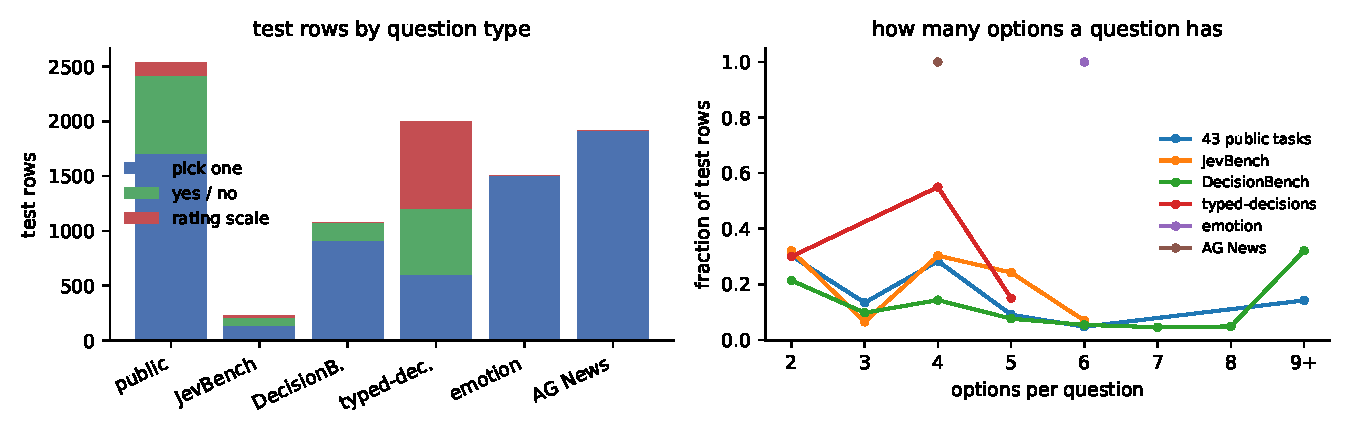
\includegraphics[width=\linewidth]{benchmarks.pdf}
\caption{The six benchmarks' test rows, by question type (left) and by the number of options a question offers (right, as a share of that benchmark's rows).}
\label{fig:bench}
\end{figure}

\subsection{Protocol and statistics}
Every method learns from its pool's feedback rows (or their labels) and is scored on the test rows. On JevBench, which has no training split, every method including the answer-key arms learns by 5-fold cross-fitting with all paraphrases of a question kept in one fold, and the calibration fifth of each training fold is drawn by paraphrase group. The feedback rows of each task are split 80 / 20 into training and calibration rows with a fixed permutation. Stochastic methods run with seeds 0, 1 and 2. Gains are paired differences in per-row correctness between two methods on the same rows, in points. Their 95\% intervals come from a bootstrap that resamples the training seeds of each side with replacement and then resamples rows by cluster: tasks on the public menu (which is macro-averaged over tasks) and DecisionBench, cases on typed-decisions, paraphrase groups on JevBench. With three seeds the seed component is itself an underestimate, so the intervals are still optimistic. Two-sided $p$-values come from the same bootstrap and are Holm-adjusted within each family of comparisons a reader is likely to count (a method against the base model across benchmarks; \pk{} against each answer-key arm across benchmarks; the KL contrasts). ``Non-inferior'' means the interval's lower bound is above $-2$ points. Same-seed reruns on different machines move individual results by up to 3 points (the earlier grid's typed-decisions seed 2 moved by 3.1), so the three-seed means, not single seeds, are what reproduce. Accuracy, ECE (15 equal-width bins, as in the README), NLL, Brier, AURC, macro-F1 and the per-benchmark slices come from the harness's \texttt{score\_metrics}.

\subsection{Methods compared}
\begin{itemize}
\item \textbf{Released model}: Vega 0.8B, Vega 4B, Laya, replayed on cached inputs and checked against the official prediction call and the README numbers. On typed-decisions, Vega also with its shipped adapters off.
\item \textbf{Their own recipe}: for Vega, VegaML's TTT head trained on the labelled feedback rows of each task, under the vegaml 0.8.0 rule (a head replaces the engine where its cross-validated accuracy beats chance) and the 0.12.3 rule (where it also beats the engine on the same rows); for Laya, the released \texttt{laya-typed-decisions} checkpoint on every benchmark, in-domain only on typed-decisions.
\item \textbf{Answer-key add-on, same recipe}: the same adapter (Vega) or head copy (Laya) trained with cross-entropy on the labels of the same rows, the same KL term, eight passes, then label-based temperature scaling; also run for one pass. In the first version the Laya head was trained without the KL term; it now matches Vega's.
\item \textbf{Answer-key add-on, early-stopped}: the same run with the epoch chosen by argmax accuracy on the calibration rows' labels. This is the tuned labelled reference the first version lacked.
\item \textbf{Answer-key fine-tune, encoder unfrozen} (Laya): head and encoder trained with cross-entropy, the same KL term, rows and passes as the encoder-unfrozen \pk{}; with and without early stopping.
\item \textbf{Label prior}: one log-offset per (task, option text) on the released probabilities, no input features, trained with \pk{}'s own loop from verdicts (learning rate chosen on the calibration rows' verdicts) and, separately, from the labels.
\item \textbf{Released model + temperature}: the released model with the honesty fix applied to its own sampled answers on its calibration rows, and with a label-fitted temperature.
\item \textbf{\pk{}} with eight passes and with one pass; head only and encoder unfrozen on Laya; without the KL term; with the switch; pooled.
\item \textbf{Realistic feedback}: the released model's best answers rated once and learned off-policy (a verdict of 1 is a label, a verdict of 0 rules that answer out); its sampled answers rated once and learned with clipped importance weights; eight-pass \pk{} with 20\% of verdicts flipped, with only half of the answers rated, and with every wrong answer reported but only 20\% of right ones.
\end{itemize}

\subsection{Compute and reproducibility}
The grid (6 benchmarks $\times$ 3 models $\times$ methods $\times$ 3 seeds, 540 steps) ran on one NVIDIA A40 from cached backbone features. One script, \texttt{experiments/peekaboo\_remaining/run.py}, runs every step, skips finished ones and retries failures; \texttt{analysis.py} computes everything in this paper from the per-row records; \texttt{paper/make\_figures.py} writes every table, figure and number in the text, so the prose cannot drift from the results. The first version's results stay in the repository under \texttt{output/}.

\section{Results}
\label{sec:results}

\subsection{Eight passes: verdicts against labels, and against the vendors' own recipes}
\label{sec:eight}

\begin{figure}[t]\centering
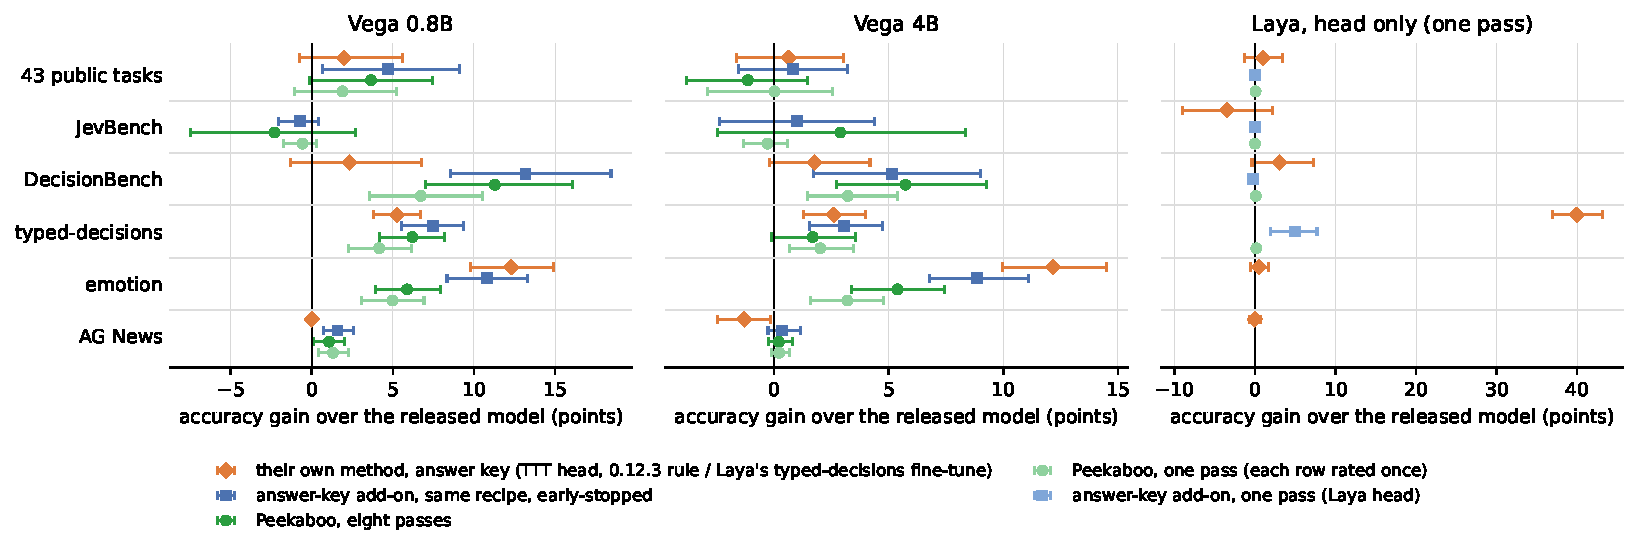
\includegraphics[width=\linewidth]{gains.pdf}
\caption{Gain over the released model on the six benchmarks, in accuracy points with 95\% intervals (seeds and row clusters resampled). Each row is a benchmark; each marker a method. Orange diamonds: the model's own labelled-data recipe (VegaML's TTT head under the 0.12.3 rule; Laya's typed-decisions fine-tune, in-domain only on typed-decisions). Blue squares: our add-on trained on the labels, early-stopped. Dark green: \pk{} with eight passes; light green: \pk{} with one pass, each row rated once. On Laya the head-only arms were run for one pass only (light blue: the labelled head, one pass). On JevBench every method is cross-fitted.}
\label{fig:gains}
\end{figure}

\begin{table}[tbp]\centering\scriptsize
\caption{Accuracy, mean over 3 seeds ($\pm$ s.d.) where a method is stochastic. JevBench has no training split: every method learns by 5-fold cross-fitting there, and pooled Peekaboo never sees it.}
\label{tab:acc}
\setlength{\tabcolsep}{2.5pt}
\resizebox{\linewidth}{!}{\begin{tabular}{llrrrrrrr}
\toprule
model & method & learns from & public & JevBench & DecisionB. & typed-dec. & emotion & AG News \\
\midrule
Vega 0.8B & released model & none & 0.556 & 0.545 & 0.509 & 0.666 & 0.568 & 0.901 \\
 & TTT head, 0.8.0 rule & answer key & 0.516 & $\cdot$ & 0.530 & 0.719 & 0.691 & 0.900 \\
 & TTT head, 0.12.3 rule & answer key & 0.576 & $\cdot$ & 0.532 & 0.719 & 0.691 & 0.901 \\
 & answer-key adapter, same recipe & answer key & 0.590 {\scriptsize$\pm$0.004} & 0.537 {\scriptsize$\pm$0.020} & 0.632 {\scriptsize$\pm$0.004} & 0.737 {\scriptsize$\pm$0.002} & 0.679 {\scriptsize$\pm$0.007} & 0.901 {\scriptsize$\pm$0.003} \\
 & answer-key adapter, early-stopped & answer key & 0.603 {\scriptsize$\pm$0.010} & 0.538 {\scriptsize$\pm$0.005} & 0.641 {\scriptsize$\pm$0.010} & 0.740 {\scriptsize$\pm$0.003} & 0.676 {\scriptsize$\pm$0.006} & 0.917 {\scriptsize$\pm$0.002} \\
 & answer-key adapter, one pass & answer key & 0.592 {\scriptsize$\pm$0.003} & 0.540 {\scriptsize$\pm$0.002} & 0.608 {\scriptsize$\pm$0.007} & 0.734 {\scriptsize$\pm$0.007} & 0.635 {\scriptsize$\pm$0.002} & 0.917 {\scriptsize$\pm$0.002} \\
 & \textbf{Peekaboo}, eight passes & verdicts & 0.593 {\scriptsize$\pm$0.013} & 0.522 {\scriptsize$\pm$0.010} & 0.622 {\scriptsize$\pm$0.002} & 0.728 {\scriptsize$\pm$0.007} & 0.627 {\scriptsize$\pm$0.004} & 0.912 {\scriptsize$\pm$0.004} \\
 & \textbf{Peekaboo}, one pass & verdicts & 0.575 {\scriptsize$\pm$0.008} & 0.540 {\scriptsize$\pm$0.002} & 0.576 {\scriptsize$\pm$0.011} & 0.708 {\scriptsize$\pm$0.003} & 0.618 {\scriptsize$\pm$0.006} & 0.914 {\scriptsize$\pm$0.002} \\
 & logged best answers, rated once & verdicts & $\cdot$ & $\cdot$ & 0.583 {\scriptsize$\pm$0.009} & 0.726 & 0.603 & $\cdot$ \\
 & Peekaboo, no KL term & verdicts & 0.582 & 0.517 {\scriptsize$\pm$0.014} & 0.609 {\scriptsize$\pm$0.004} & 0.709 & 0.622 & 0.916 \\
\addlinespace
Vega 4B & released model & none & 0.718 & 0.667 & 0.636 & 0.729 & 0.575 & 0.928 \\
 & TTT head, 0.8.0 rule & answer key & 0.678 & $\cdot$ & 0.640 & 0.757 & 0.697 & 0.915 \\
 & TTT head, 0.12.3 rule & answer key & 0.724 & $\cdot$ & 0.654 & 0.755 & 0.697 & 0.915 \\
 & answer-key adapter, same recipe & answer key & 0.706 {\scriptsize$\pm$0.002} & 0.706 {\scriptsize$\pm$0.011} & 0.687 {\scriptsize$\pm$0.007} & 0.769 {\scriptsize$\pm$0.001} & 0.640 {\scriptsize$\pm$0.001} & 0.924 {\scriptsize$\pm$0.003} \\
 & answer-key adapter, early-stopped & answer key & 0.726 {\scriptsize$\pm$0.005} & 0.677 {\scriptsize$\pm$0.010} & 0.688 {\scriptsize$\pm$0.005} & 0.760 {\scriptsize$\pm$0.008} & 0.663 {\scriptsize$\pm$0.004} & 0.931 {\scriptsize$\pm$0.004} \\
 & answer-key adapter, one pass & answer key & 0.723 {\scriptsize$\pm$0.003} & 0.667 {\scriptsize$\pm$0.000} & 0.683 {\scriptsize$\pm$0.009} & 0.775 {\scriptsize$\pm$0.008} & 0.631 {\scriptsize$\pm$0.004} & 0.931 {\scriptsize$\pm$0.003} \\
 & \textbf{Peekaboo}, eight passes & verdicts & 0.706 {\scriptsize$\pm$0.005} & 0.696 {\scriptsize$\pm$0.005} & 0.694 {\scriptsize$\pm$0.005} & 0.746 {\scriptsize$\pm$0.010} & 0.629 {\scriptsize$\pm$0.009} & 0.930 {\scriptsize$\pm$0.002} \\
 & \textbf{Peekaboo}, one pass & verdicts & 0.718 {\scriptsize$\pm$0.017} & 0.664 {\scriptsize$\pm$0.003} & 0.669 {\scriptsize$\pm$0.004} & 0.749 {\scriptsize$\pm$0.004} & 0.607 {\scriptsize$\pm$0.003} & 0.930 {\scriptsize$\pm$0.002} \\
 & logged best answers, rated once & verdicts & $\cdot$ & $\cdot$ & 0.655 {\scriptsize$\pm$0.004} & 0.769 & 0.611 & $\cdot$ \\
 & Peekaboo, no KL term & verdicts & 0.713 & 0.693 & 0.672 {\scriptsize$\pm$0.002} & 0.742 & 0.519 & 0.928 \\
\addlinespace
Laya & released model & none & 0.540 & 0.576 & 0.406 & 0.362 & 0.599 & 0.930 \\
 & laya-typed-decisions (fine-tune on typed-decisions) & answer key & 0.550 & 0.541 & 0.436 & 0.761 & 0.604 & 0.930 \\
 & answer-key head, one pass & answer key & 0.541 & 0.576 & 0.403 & 0.412 {\scriptsize$\pm$0.011} & $\cdot$ & $\cdot$ \\
 & \textbf{Peekaboo}, head only, one pass & verdicts & 0.541 & 0.576 & 0.406 & 0.364 {\scriptsize$\pm$0.003} & $\cdot$ & $\cdot$ \\
 & answer-key fine-tune, encoder unfrozen & answer key & 0.587 {\scriptsize$\pm$0.009} & 0.535 {\scriptsize$\pm$0.025} & 0.560 {\scriptsize$\pm$0.016} & 0.750 & 0.899 & $\cdot$ \\
 & answer-key fine-tune, encoder unfrozen, early-stopped & answer key & 0.584 {\scriptsize$\pm$0.003} & 0.595 {\scriptsize$\pm$0.005} & 0.554 {\scriptsize$\pm$0.005} & 0.750 & 0.905 & $\cdot$ \\
 & \textbf{Peekaboo}, encoder unfrozen, eight passes & verdicts & 0.566 {\scriptsize$\pm$0.001} & 0.558 {\scriptsize$\pm$0.030} & 0.545 {\scriptsize$\pm$0.014} & 0.685 & 0.820 & $\cdot$ \\
 & \textbf{Peekaboo}, encoder unfrozen, one pass & verdicts & 0.562 {\scriptsize$\pm$0.005} & 0.573 {\scriptsize$\pm$0.005} & 0.482 {\scriptsize$\pm$0.026} & 0.588 & 0.698 & $\cdot$ \\
\bottomrule
\end{tabular}}
\end{table}

\begin{table}[tbp]\centering\scriptsize
\caption{Gain over the released model in accuracy points, with 95\% intervals that resample seeds and row clusters; $\dagger$ marks differences that survive Holm adjustment within the method's family. JevBench has no training split: every method learns by 5-fold cross-fitting there, and pooled Peekaboo never sees it.}
\label{tab:gain}
\setlength{\tabcolsep}{2.5pt}
\resizebox{\linewidth}{!}{\begin{tabular}{llrrrrrrr}
\toprule
model & method & learns from & public & JevBench & DecisionB. & typed-dec. & emotion & AG News \\
\midrule
Vega 0.8B & released model & none & -- & -- & -- & -- & -- & -- \\
 & TTT head, 0.8.0 rule & answer key & -4.1 & $\cdot$ & +2.1 & +5.3 & +12.3 & -0.2 \\
 & TTT head, 0.12.3 rule & answer key & +2.0 & $\cdot$ & +2.3 & +5.2 & +12.3 & +0.0 \\
 & answer-key adapter, same recipe & answer key & +3.4 & -0.9 & +12.3 & +7.0 & +11.1 & +0.0 \\
 & answer-key adapter, early-stopped & answer key & +4.7 & -0.7 & +13.2 & +7.4 & +10.8 & +1.6 \\
 & answer-key adapter, one pass & answer key & +3.6 & -0.6 & +10.0 & +6.8 & +6.6 & +1.6 \\
 & \textbf{Peekaboo}, eight passes & verdicts & +3.7 & -2.3 & +11.3$^{\dagger}$ & +6.2$^{\dagger}$ & +5.9$^{\dagger}$ & +1.1 \\
 & \textbf{Peekaboo}, one pass & verdicts & +1.9 & -0.6 & +6.7$^{\dagger}$ & +4.1$^{\dagger}$ & +5.0$^{\dagger}$ & +1.3$^{\dagger}$ \\
 & logged best answers, rated once & verdicts & $\cdot$ & $\cdot$ & +7.4 & +6.0 & +3.5 & $\cdot$ \\
 & Peekaboo, no KL term & verdicts & +2.5 & -2.9 & +10.0 & +4.2 & +5.4 & +1.5 \\
\addlinespace
Vega 4B & released model & none & -- & -- & -- & -- & -- & -- \\
 & TTT head, 0.8.0 rule & answer key & -3.9 & $\cdot$ & +0.4 & +2.8 & +12.2 & -1.3 \\
 & TTT head, 0.12.3 rule & answer key & +0.6 & $\cdot$ & +1.8 & +2.6 & +12.2 & -1.3 \\
 & answer-key adapter, same recipe & answer key & -1.2 & +3.9 & +5.1 & +4.0 & +6.5 & -0.3 \\
 & answer-key adapter, early-stopped & answer key & +0.8 & +1.0 & +5.1 & +3.0 & +8.8 & +0.3 \\
 & answer-key adapter, one pass & answer key & +0.5 & -0.0 & +4.7 & +4.6 & +5.7 & +0.3 \\
 & \textbf{Peekaboo}, eight passes & verdicts & -1.1 & +2.9 & +5.7$^{\dagger}$ & +1.7 & +5.4$^{\dagger}$ & +0.2 \\
 & \textbf{Peekaboo}, one pass & verdicts & +0.0 & -0.3 & +3.2$^{\dagger}$ & +2.0$^{\dagger}$ & +3.2$^{\dagger}$ & +0.2 \\
 & logged best answers, rated once & verdicts & $\cdot$ & $\cdot$ & +1.8 & +4.0 & +3.6 & $\cdot$ \\
 & Peekaboo, no KL term & verdicts & -0.5 & +2.6 & +3.5 & +1.3 & -5.6 & +0.0 \\
\addlinespace
Laya & released model & none & -- & -- & -- & -- & -- & -- \\
 & laya-typed-decisions (fine-tune on typed-decisions) & answer key & +1.0 & -3.5 & +3.1 & +40.0 & +0.5 & +0.0 \\
 & answer-key head, one pass & answer key & +0.1 & +0.0 & -0.3 & +5.0 & $\cdot$ & $\cdot$ \\
 & \textbf{Peekaboo}, head only, one pass & verdicts & +0.1 & +0.0 & +0.1 & +0.2 & $\cdot$ & $\cdot$ \\
 & answer-key fine-tune, encoder unfrozen & answer key & +4.6 & -4.0 & +15.4 & +38.8 & +30.0 & $\cdot$ \\
 & answer-key fine-tune, encoder unfrozen, early-stopped & answer key & +4.3 & +1.9 & +14.8 & +38.8 & +30.6 & $\cdot$ \\
 & \textbf{Peekaboo}, encoder unfrozen, eight passes & verdicts & +2.6 & -1.7 & +14.0$^{\dagger}$ & +32.3$^{\dagger}$ & +22.2$^{\dagger}$ & $\cdot$ \\
 & \textbf{Peekaboo}, encoder unfrozen, one pass & verdicts & +2.1 & -0.3 & +7.7 & +22.6 & +9.9 & $\cdot$ \\
\bottomrule
\end{tabular}}
\end{table}

\begin{table}[tbp]\centering\scriptsize
\caption{Head to head, in accuracy points with 95\% intervals (seeds and row clusters resampled). Positive means the first method is better. $\dagger$: survives Holm adjustment within the row's family; NI: non-inferior at a 2-point margin (lower bound above $-2$). TTT is scored under the vegaml 0.12.3 rule; for Laya ``their method'' is the typed-decisions fine-tune, in-domain only on typed-decisions.}
\label{tab:h2h}
\setlength{\tabcolsep}{3pt}
\resizebox{\linewidth}{!}{\begin{tabular}{llrrrrrr}
\toprule
model & comparison & public & JevBench & DecisionB. & typed-dec. & emotion & AG News \\
\midrule
\multicolumn{8}{l}{\textit{Vega 0.8B}} \\
 & Peekaboo (8 passes) vs. their method & +1.7 {\scriptsize[-1.6, +5.0]} & -- & +9.0 {\scriptsize[+5.4, +12.6]} & +0.9 {\scriptsize[-0.7, +2.7]} & -6.4 {\scriptsize[-8.4, -4.3]} & +1.1 {\scriptsize[+0.1, +2.0]} \\
 & Peekaboo (8) vs. answer key, same recipe (8) & +0.3 {\scriptsize[-2.8, +3.6]} & -1.4 {\scriptsize[-6.1, +3.0]} & -1.0 {\scriptsize[-3.0, +1.0]} & -0.9 {\scriptsize[-2.2, +0.5]} & -5.2 {\scriptsize[-7.1, -3.3]}$^{\dagger}$ & +1.0 {\scriptsize[-0.1, +2.1]} NI \\
 & Peekaboo (8) vs. answer key, early-stopped & -1.1 {\scriptsize[-4.0, +2.0]} & -1.6 {\scriptsize[-7.0, +3.5]} & -1.9 {\scriptsize[-4.1, +0.3]} & -1.3 {\scriptsize[-2.6, +0.1]} & -4.9 {\scriptsize[-6.8, -3.0]} & -0.5 {\scriptsize[-1.3, +0.2]} NI \\
 & Peekaboo (1 pass) vs. answer key (1 pass) & -1.7 {\scriptsize[-3.7, +0.5]} & -0.0 {\scriptsize[-1.0, +1.0]} NI & -3.2 {\scriptsize[-5.8, -0.6]} & -2.7 {\scriptsize[-4.1, -1.2]} & -1.7 {\scriptsize[-3.0, -0.4]} & -0.3 {\scriptsize[-0.9, +0.4]} NI \\
 & Peekaboo, 1 pass vs. 8 passes & -1.8 {\scriptsize[-4.4, +0.8]} & +1.7 {\scriptsize[-3.2, +7.2]} & -4.6 {\scriptsize[-8.1, -1.4]} & -2.1 {\scriptsize[-3.6, -0.4]} & -0.9 {\scriptsize[-2.4, +0.5]} & +0.2 {\scriptsize[-0.5, +1.0]} \\
 & logged best answers vs. Peekaboo (1 pass) & -- & -- & +0.7 {\scriptsize[-2.4, +3.7]} & +1.9 {\scriptsize[+0.3, +3.5]} NI & -1.5 {\scriptsize[-4.1, +0.7]} & -- \\
 & KL term vs. none & +1.1 {\scriptsize[-1.5, +3.9]} & +0.6 {\scriptsize[-2.4, +3.7]} & +1.2 {\scriptsize[-0.6, +3.0]} & +1.9 {\scriptsize[+0.3, +3.5]} & +0.5 {\scriptsize[-1.0, +1.8]} & -0.5 {\scriptsize[-1.3, +0.3]} \\
 & with the switch vs. without & +0.0 {\scriptsize[-2.2, +2.3]} & +2.3 {\scriptsize[-2.9, +7.7]} & +0.0 {\scriptsize[-1.2, +1.1]} & +0.0 {\scriptsize[-1.2, +1.3]} & +0.0 {\scriptsize[-1.1, +1.1]} & +0.0 {\scriptsize[-0.7, +0.7]} \\
\midrule
\multicolumn{8}{l}{\textit{Vega 4B}} \\
 & Peekaboo (8 passes) vs. their method & -1.8 {\scriptsize[-4.3, +0.7]} & -- & +4.0 {\scriptsize[+1.5, +6.5]} & -0.9 {\scriptsize[-2.6, +0.9]} & -6.8 {\scriptsize[-8.9, -4.7]} & +1.5 {\scriptsize[+0.4, +2.6]} \\
 & Peekaboo (8) vs. answer key, same recipe (8) & +0.0 {\scriptsize[-2.0, +2.0]} & -1.0 {\scriptsize[-5.0, +2.8]} & +0.6 {\scriptsize[-1.6, +2.7]} NI & -2.3 {\scriptsize[-3.8, -0.8]}$^{\dagger}$ & -1.1 {\scriptsize[-3.2, +1.0]} & +0.6 {\scriptsize[-0.1, +1.3]} NI \\
 & Peekaboo (8) vs. answer key, early-stopped & -2.0 {\scriptsize[-4.0, -0.2]} & +1.9 {\scriptsize[-2.7, +6.6]} & +0.6 {\scriptsize[-1.2, +2.3]} NI & -1.4 {\scriptsize[-2.9, +0.4]} & -3.5 {\scriptsize[-5.3, -1.7]} & -0.1 {\scriptsize[-0.8, +0.5]} NI \\
 & Peekaboo (1 pass) vs. answer key (1 pass) & -0.5 {\scriptsize[-3.0, +1.4]} & -0.3 {\scriptsize[-1.4, +0.7]} NI & -1.4 {\scriptsize[-3.8, +0.8]} & -2.6 {\scriptsize[-4.0, -1.2]} & -2.5 {\scriptsize[-3.7, -1.2]} & -0.1 {\scriptsize[-0.7, +0.5]} NI \\
 & Peekaboo, 1 pass vs. 8 passes & +1.2 {\scriptsize[-1.3, +3.5]} & -3.2 {\scriptsize[-8.7, +2.4]} & -2.5 {\scriptsize[-5.8, +0.0]} & +0.3 {\scriptsize[-1.2, +1.9]} & -2.2 {\scriptsize[-3.8, -0.5]} & +0.0 {\scriptsize[-0.6, +0.5]} \\
 & logged best answers vs. Peekaboo (1 pass) & -- & -- & -1.4 {\scriptsize[-4.4, +1.9]} & +2.0 {\scriptsize[+0.7, +3.4]} NI & +0.4 {\scriptsize[-1.9, +2.6]} NI & -- \\
 & KL term vs. none & -0.6 {\scriptsize[-2.8, +1.4]} & +0.3 {\scriptsize[-3.1, +3.8]} & +2.2 {\scriptsize[+0.4, +4.2]} & +0.4 {\scriptsize[-1.5, +2.3]} & +11.0 {\scriptsize[+8.5, +13.5]}$^{\dagger}$ & +0.2 {\scriptsize[-0.2, +0.8]} \\
 & with the switch vs. without & +0.0 {\scriptsize[-1.3, +1.2]} & -2.7 {\scriptsize[-8.1, +2.5]} & +0.0 {\scriptsize[-1.1, +1.2]} & -0.7 {\scriptsize[-3.0, +1.5]} & +0.0 {\scriptsize[-1.5, +1.6]} & +0.0 {\scriptsize[-0.5, +0.4]} \\
\midrule
\multicolumn{8}{l}{\textit{Laya}} \\
 & Peekaboo, head (1) vs. answer-key head (1) & +0.0 {\scriptsize[-0.3, +0.3]} NI & +0.0 {\scriptsize[+0.0, +0.0]} NI & +0.4 {\scriptsize[+0.1, +0.7]} NI & -4.8 {\scriptsize[-7.5, -2.0]} & -- & -- \\
 & Peekaboo, encoder (8) vs. their fine-tune & +1.6 {\scriptsize[-2.1, +5.3]} & +1.7 {\scriptsize[-4.7, +8.8]} & +10.9 {\scriptsize[+4.7, +16.7]}$^{\dagger}$ & -7.6 {\scriptsize[-9.8, -5.4]}$^{\dagger}$ & +21.6 {\scriptsize[+19.4, +24.0]}$^{\dagger}$ & -- \\
 & Peekaboo, encoder (8) vs. answer-key encoder, same recipe & -2.1 {\scriptsize[-5.1, +0.7]} & +2.3 {\scriptsize[-3.9, +7.9]} & -1.4 {\scriptsize[-5.1, +2.0]} & -6.5 {\scriptsize[-8.7, -4.1]}$^{\dagger}$ & -7.9 {\scriptsize[-9.6, -6.1]}$^{\dagger}$ & -- \\
 & Peekaboo, encoder (8) vs. answer-key encoder, early-stopped & -1.8 {\scriptsize[-4.7, +0.9]} & -3.6 {\scriptsize[-8.7, +1.4]} & -0.9 {\scriptsize[-4.5, +2.0]} & -6.5 {\scriptsize[-8.7, -4.3]} & -8.4 {\scriptsize[-10.2, -6.7]} & -- \\
 & Peekaboo, encoder: 1 pass vs. 8 & -0.4 {\scriptsize[-3.0, +2.1]} & +1.4 {\scriptsize[-4.4, +6.9]} & -6.3 {\scriptsize[-11.1, -1.9]} & -9.7 {\scriptsize[-12.1, -7.1]} & -12.2 {\scriptsize[-14.2, -10.3]} & -- \\
\bottomrule
\end{tabular}}
\end{table}


Tables~\ref{tab:acc} and \ref{tab:gain} give accuracy and gain over the released model for every arm, Table~\ref{tab:h2h} the paired head-to-heads, and Figure~\ref{fig:gains} the picture. Under the eight-pass protocol the verdict-trained add-on lands close to the same add-on trained on labels and early-stopped, and mostly below it. On DecisionBench \pk{} gains $\gainSmallPkDb$ points at 0.8B and $\gainBigPkDb$ at 4B; the early-stopped labelled adapter gains $\gainSmallSupEsDb$ and $\gainBigSupEsDb$. The paired difference is $\gainSmallPkDbVsSupEs$ $\ciSmallPkDbVsSupEs$ at 0.8B and $\gainBigPkDbVsSupEs$ $\ciBigPkDbVsSupEs$ at 4B; on typed-decisions $\gainSmallPkTypedVsSupEs$ and $\gainBigPkTypedVsSupEs$, on the public menu $\gainSmallPkPubVsSupEs$ and $\gainBigPkPubVsSupEs$, on AG News $\gainSmallPkAgVsSupEs$ and $\gainBigPkAgVsSupEs$, on JevBench $\gainSmallPkJevVsSupEs$ and $\gainBigPkJevVsSupEs$. Emotion is the exception: $\gainSmallPkEmoVsSupEs$ $\ciSmallPkEmoVsSupEs$ and $\gainBigPkEmoVsSupEs$ $\ciBigPkEmoVsSupEs$, and these two are the only differences in the family that survive Holm adjustment. Against the same-recipe adapter without early stopping the differences are smaller still. This is what the $\pi(y)$ weighting predicts for a protocol that reveals most labels (Section~\ref{sec:anatomy}): the two arms then optimise nearly the same objective. The first version read these gaps as ``the bit is nearly as good as the label''; the accurate reading is that eight rounds of verdicts on the same rows are nearly as good as the labels, because they mostly are the labels. The one-rating arms below measure a single verdict.

\paragraph{Against VegaML's TTT head.}
Under the 0.12.3 rule, which keeps a head only where it beats the engine on its own fit rows, the TTT head gains $\gainSmallTttGuardPub$ and $\gainBigTttGuardPub$ on the public menu; under the 0.8.0 rule it lost $\absSmallTttPub$ and $\absBigTttPub$ points, the losses our first version counted as wins. \pk{} minus the guarded TTT head is $\gainSmallPkDbVsTttGuard$ $\ciSmallPkDbVsTttGuard$ on DecisionBench at 0.8B and $\gainBigPkDbVsTttGuard$ $\ciBigPkDbVsTttGuard$ at 4B; $\gainSmallPkAgVsTttGuard$ $\ciSmallPkAgVsTttGuard$ and $\gainBigPkAgVsTttGuard$ $\ciBigPkAgVsTttGuard$ on AG News; $\gainSmallPkPubVsTttGuard$ $\ciSmallPkPubVsTttGuard$ and $\gainBigPkPubVsTttGuard$ $\ciBigPkPubVsTttGuard$ on the public menu; $\gainSmallPkTypedVsTttGuard$ and $\gainBigPkTypedVsTttGuard$ on typed-decisions; and $\gainSmallPkEmoVsTttGuard$ $\ciSmallPkEmoVsTttGuard$ and $\gainBigPkEmoVsTttGuard$ $\ciBigPkEmoVsTttGuard$ on emotion. After Holm adjustment the verdict-trained adapter is ahead of VegaML's labelled recipe on DecisionBench at both sizes and on AG News at 4B, level on the public menu and typed-decisions, and behind on emotion at both sizes. On DecisionBench the guarded head answers $\tttCoveredSmallDb$ of 1,075 rows at 0.8B and $\tttCoveredBigDb$ at 4B (Table~\ref{tab:ttt}). On the rows it answers, \pk{} minus TTT is $\gainPeekabooVsTttCoveredSmallDb$ $\ciPeekabooVsTttCoveredSmallDb$ and $\gainPeekabooVsTttCoveredBigDb$ $\ciPeekabooVsTttCoveredBigDb$, neither significant, and the labelled adapter does about as well there ($\gainAdapterVsTttCoveredSmallDb$, $\gainAdapterVsTttCoveredBigDb$). The significant margin is on the rows the head leaves to the engine ($\gainPeekabooVsTttUncoveredSmallDb$ and $\gainPeekabooVsTttUncoveredBigDb$), where it is a comparison with the released model, and it belongs to an in-engine adapter that reads the option text, not to the feedback signal. Emotion goes to TTT by a wide margin: a six-way single-label task with 3,200 labelled rows is where a logistic head on good features is at its best.

\paragraph{JevBench.}
With every arm cross-fitted, the answer-key adapter is defined on JevBench too, which removes the first version's claim that \pk{} was the only method to improve Vega 4B there. At 4B \pk{} gains $\gainBigPkJev$ $\ciBigPkJev$ and the labelled adapter $\gainBigSupJev$ $\ciBigSupJev$; at 0.8B \pk{} loses $\absSmallPkJev$ points and the labelled adapter $\absSmallSupJev$. None of these intervals excludes zero. JevBench has 231 rows and 38-to-42-row calibration folds.

\subsection{One rating per row, and feedback as a deployment delivers it}
\label{sec:realistic}

\begin{figure}[t]\centering
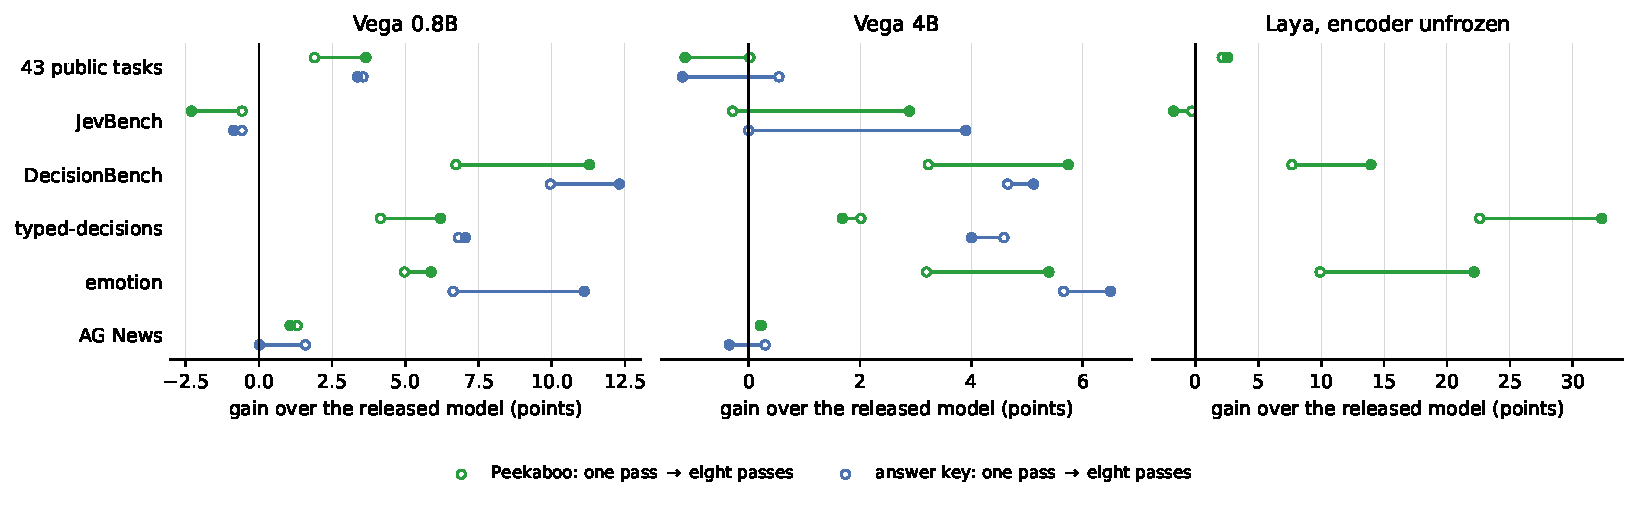
\includegraphics[width=\linewidth]{passes.pdf}
\caption{One pass (open markers) against eight (filled), for \pk{} (green) and the answer-key add-on (blue), as gain over the released model. One pass rates each row once and takes one eighth of the gradient steps. Laya: the encoder-unfrozen \pk{} only.}
\label{fig:passes}
\end{figure}

\begin{table}[tbp]\centering\small
\caption{Feedback as a deployment delivers it: gain over the released model in points (95\% intervals), on the three benchmarks with the realistic-feedback arms.}
\label{tab:realistic}
\setlength{\tabcolsep}{3pt}
\resizebox{\linewidth}{!}{\begin{tabular}{lrrrrrrrrr}
\toprule
feedback & \multicolumn{3}{c}{DecisionBench} & \multicolumn{3}{c}{typed-decisions} & \multicolumn{3}{c}{emotion} \\
 & Vega 0.8B & Vega 4B & Laya (head) & Vega 0.8B & Vega 4B & Laya (head) & Vega 0.8B & Vega 4B & Laya (head) \\
\midrule
eight passes, clean verdicts & +11.3 {\scriptsize[+7.0, +16.1]} & +5.7 {\scriptsize[+2.7, +9.3]} & -- & +6.2 {\scriptsize[+4.2, +8.2]} & +1.7 {\scriptsize[-0.1, +3.6]} & -- & +5.9 {\scriptsize[+3.9, +8.0]} & +5.4 {\scriptsize[+3.4, +7.4]} & -- \\
one pass, clean verdicts & +6.7 {\scriptsize[+3.6, +10.5]} & +3.2 {\scriptsize[+1.5, +5.4]} & +0.1 {\scriptsize[+0.0, +0.3]} & +4.1 {\scriptsize[+2.2, +6.1]} & +2.0 {\scriptsize[+0.7, +3.5]} & +0.2 {\scriptsize[-0.2, +0.5]} & +5.0 {\scriptsize[+3.1, +6.9]} & +3.2 {\scriptsize[+1.6, +4.8]} & -- \\
logged: the released model's best answers, rated once & +7.4 {\scriptsize[+3.4, +12.2]} & +1.8 {\scriptsize[-1.4, +5.3]} & -- & +6.0 {\scriptsize[+3.9, +8.2]} & +4.0 {\scriptsize[+2.5, +5.7]} & -- & +3.5 {\scriptsize[+0.7, +6.2]} & +3.6 {\scriptsize[+1.2, +5.9]} & -- \\
logged: the released model's sampled answers, rated once (clipped IPS) & +8.3 {\scriptsize[+4.4, +13.0]} & +4.3 {\scriptsize[+1.6, +7.3]} & -- & +5.6 {\scriptsize[+3.5, +7.6]} & +1.8 {\scriptsize[+0.1, +3.8]} & -- & +6.6 {\scriptsize[+4.6, +8.6]} & +4.5 {\scriptsize[+2.5, +6.6]} & -- \\
20\% of verdicts flipped (eight passes) & +9.1 {\scriptsize[+5.8, +12.8]} & +4.2 {\scriptsize[+1.7, +7.3]} & -- & +5.9 {\scriptsize[+4.2, +7.5]} & +2.8 {\scriptsize[+1.2, +4.3]} & -- & +4.7 {\scriptsize[+3.1, +6.3]} & +4.7 {\scriptsize[+2.7, +6.8]} & -- \\
half of the answers rated (eight passes) & +10.3 {\scriptsize[+6.2, +14.8]} & +4.7 {\scriptsize[+1.6, +8.3]} & -- & +5.2 {\scriptsize[+3.1, +7.5]} & +3.5 {\scriptsize[+1.8, +5.3]} & -- & +6.5 {\scriptsize[+4.2, +8.9]} & +0.0 {\scriptsize[+0.0, +0.0]} & -- \\
every wrong answer reported, 20\% of right ones (eight passes) & +10.0 {\scriptsize[+6.0, +14.7]} & +5.7 {\scriptsize[+2.7, +9.1]} & -- & +7.0 {\scriptsize[+5.0, +9.0]} & +4.2 {\scriptsize[+2.4, +5.9]} & -- & +6.7 {\scriptsize[+4.5, +9.0]} & +2.7 {\scriptsize[+0.9, +4.5]} & -- \\
answer key, one pass & +10.0 {\scriptsize[+6.3, +13.9]} & +4.7 {\scriptsize[+2.1, +7.4]} & -0.3 {\scriptsize[-0.7, +0.0]} & +6.8 {\scriptsize[+4.8, +8.8]} & +4.6 {\scriptsize[+3.0, +6.4]} & +5.0 {\scriptsize[+1.9, +7.7]} & +6.6 {\scriptsize[+4.5, +8.8]} & +5.7 {\scriptsize[+3.8, +7.7]} & -- \\
answer key, eight passes & +12.3 {\scriptsize[+7.8, +17.5]} & +5.1 {\scriptsize[+1.4, +9.1]} & -- & +7.0 {\scriptsize[+5.0, +9.1]} & +4.0 {\scriptsize[+2.5, +5.6]} & -- & +11.1 {\scriptsize[+8.6, +13.6]} & +6.5 {\scriptsize[+4.3, +8.8]} & -- \\
\bottomrule
\end{tabular}}
\end{table}


\begin{figure}[t]\centering
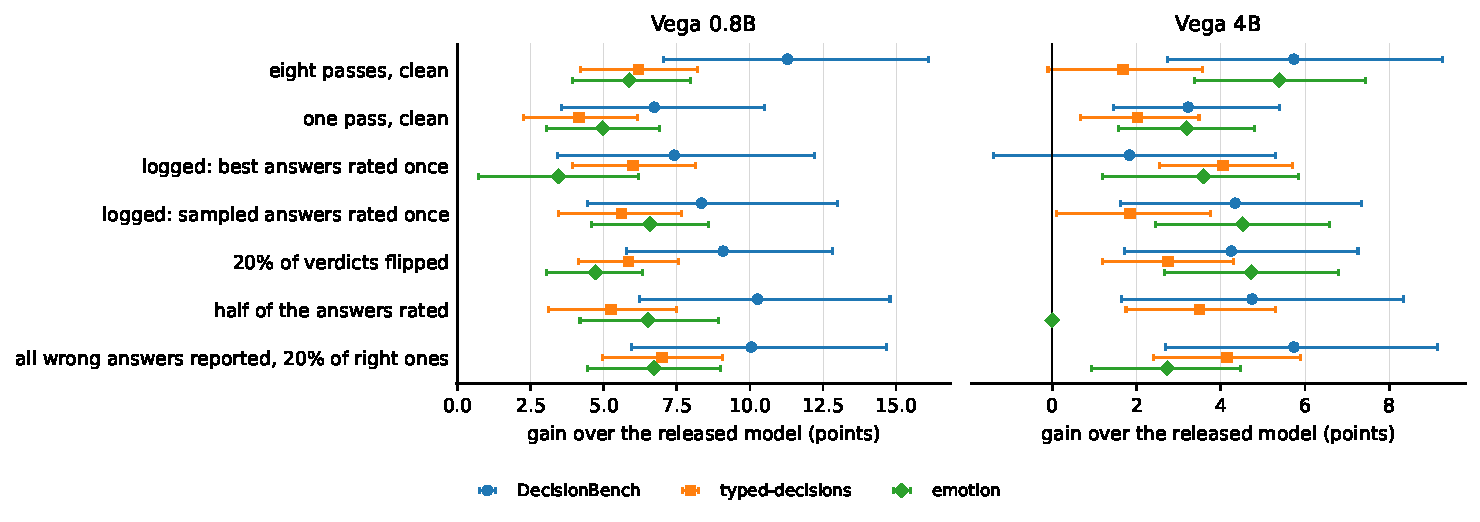
\includegraphics[width=\linewidth]{realistic.pdf}
\caption{Feedback as a deployment delivers it, on Vega: gain over the released model with 95\% intervals for the clean eight-pass and one-pass arms, the two logged arms (one verdict per row on the released model's best or sampled answers, trained off-policy), and eight-pass \pk{} with flipped, missing or complaint-skewed verdicts. The clean arms have three seeds everywhere; the logged and damaged-feedback arms three on DecisionBench and one on typed-decisions and emotion. The half-rated emotion run at 4B failed (Section~\ref{sec:realistic}).}
\label{fig:realistic}
\end{figure}

Figure~\ref{fig:passes} shows what a single pass keeps. On DecisionBench one-pass \pk{} gains $\gainSmallPkOneDb$ $\ciSmallPkOneDb$ at 0.8B and $\gainBigPkOneDb$ $\ciBigPkOneDb$ at 4B, against $\gainSmallPkDb$ and $\gainBigPkDb$ with eight passes; the one-pass labelled adapter gains $\gainSmallSupOneDb$ and $\gainBigSupOneDb$. At matched epochs the gap between verdicts and labels is $\gainSmallPkOneDbVsSupOne$ $\ciSmallPkOneDbVsSupOne$ and $\gainBigPkOneDbVsSupOne$ $\ciBigPkOneDbVsSupOne$, wider than with eight passes. On typed-decisions one pass gives $\gainSmallPkOneTyped$ and $\gainBigPkOneTyped$ (labels: $\gainSmallSupOneTyped$, $\gainBigSupOneTyped$; verdicts significantly behind at both sizes); on the public menu $\gainSmallPkOnePub$ and $\gainBigPkOnePub$; on emotion $\gainSmallPkOneEmo$ and $\gainBigPkOneEmo$; on AG News $\gainSmallPkOneAg$ and $\gainBigPkOneAg$. One pass keeps about half to two thirds of the eight-pass gain on DecisionBench and the public menu and more on emotion.

One pass confounds two things: each row is rated once, and the model takes one eighth of the gradient steps. The logged arms separate them. Each row of the pool is answered once by the released model, rated once, and the add-on is then trained on that fixed log for eight passes, off-policy. With the released model's sampled answers and clipped importance weights this gains $\gainSmallLogIpsDb$ $\ciSmallLogIpsDb$ on DecisionBench at 0.8B and $\gainBigLogIpsDb$ $\ciBigLogIpsDb$ at 4B. Against one on-policy pass that is $\gainSmallLogIpsDbVsPkOne$ $\ciSmallLogIpsDbVsPkOne$ and $\gainBigLogIpsDbVsPkOne$ $\ciBigLogIpsDbVsPkOne$; against eight passes it is $\gainSmallLogIpsDbVsPk$ $\ciSmallLogIpsDbVsPk$ and $\gainBigLogIpsDbVsPk$ $\ciBigLogIpsDbVsPk$. So on DecisionBench, where the logged arms have three seeds, more optimisation recovers part of the one-pass shortfall and the larger part, the only significant one at 0.8B, is information: more verdicts per row. On typed-decisions and emotion, where the logged arms have one seed, the logged arm is level with eight on-policy passes ($\gainSmallLogIpsTypedVsPk$ and $\gainSmallLogIpsEmoVsPk$ at 0.8B, $\gainBigLogIpsTypedVsPk$ and $\gainBigLogIpsEmoVsPk$ at 4B). Against the early-stopped labelled adapter the logged sampled arm is $\gainSmallLogIpsDbVsSupEs$ $\ciSmallLogIpsDbVsSupEs$ on DecisionBench, $\gainSmallLogIpsTypedVsSupEs$ on typed-decisions and $\gainSmallLogIpsEmoVsSupEs$ on emotion at 0.8B, and $\gainBigLogIpsDbVsSupEs$, $\gainBigLogIpsTypedVsSupEs$ and $\gainBigLogIpsEmoVsSupEs$ at 4B: one logged verdict per row stays below the labels on every cell, significantly on four of the six.

Table~\ref{tab:realistic} and Figure~\ref{fig:realistic} collect the deployment question. A system that serves its best answer rather than a sample logs only that answer's verdict: a 1 is a label, a 0 rules one option out. Learning from that log gains $\gainSmallLogArgDb$ $\ciSmallLogArgDb$ on DecisionBench at 0.8B and $\gainBigLogArgDb$ $\ciBigLogArgDb$ at 4B, $\gainSmallLogArgTyped$ and $\gainBigLogArgTyped$ on typed-decisions, and $\gainSmallLogArgEmo$ and $\gainBigLogArgEmo$ on emotion. It trails the early-stopped labels by $\absSmallLogArgDbVsSupEs$ and $\absBigLogArgDbVsSupEs$ points on DecisionBench and by $\absSmallLogArgEmoVsSupEs$ and $\absBigLogArgEmoVsSupEs$ on emotion, and on typed-decisions at 4B it is level with them ($\gainBigLogArgTypedVsSupEs$). Neither logging policy dominates: sampled answers are worth $\gainSmallLogIpsDbVsLogArg$ and $\gainBigLogIpsDbVsLogArg$ points more on DecisionBench and $\gainSmallLogIpsEmoVsLogArg$ on emotion at 0.8B, and $\gainBigLogIpsTypedVsLogArg$ on typed-decisions at 4B.

We measured damaged feedback only under the eight-pass protocol, where a flipped or missing verdict on one pass is redrawn on the next; how noise affects a single rating per row is not measured here. On DecisionBench, with three seeds, 20\% of verdicts flipped costs $\absSmallNoiseDbVsPk$ points at 0.8B and $\absBigNoiseDbVsPk$ at 4B, half of the answers unrated $\absSmallHalfDbVsPk$ and $\absBigHalfDbVsPk$, and complaint-skewed verdicts $\absSmallComplDbVsPk$ and $\absBigComplDbVsPk$. On typed-decisions and emotion these arms have one seed against the clean arm's three and differ from it by up to three points in either direction. One run failed: with half of the answers unrated on emotion at 4B the adapter's predictions are identical to the released model's on every test row and its reward stays flat through all eight passes, so that cell ($\gainBigHalfEmo$) says nothing about missing feedback. Rewards are computed from the gold answer in all of these; a rater who is systematically wrong about what was right is not simulated beyond the flipped verdicts.

\subsection{What the gain is made of}
\label{sec:anatomy}

\begin{figure}[t]\centering
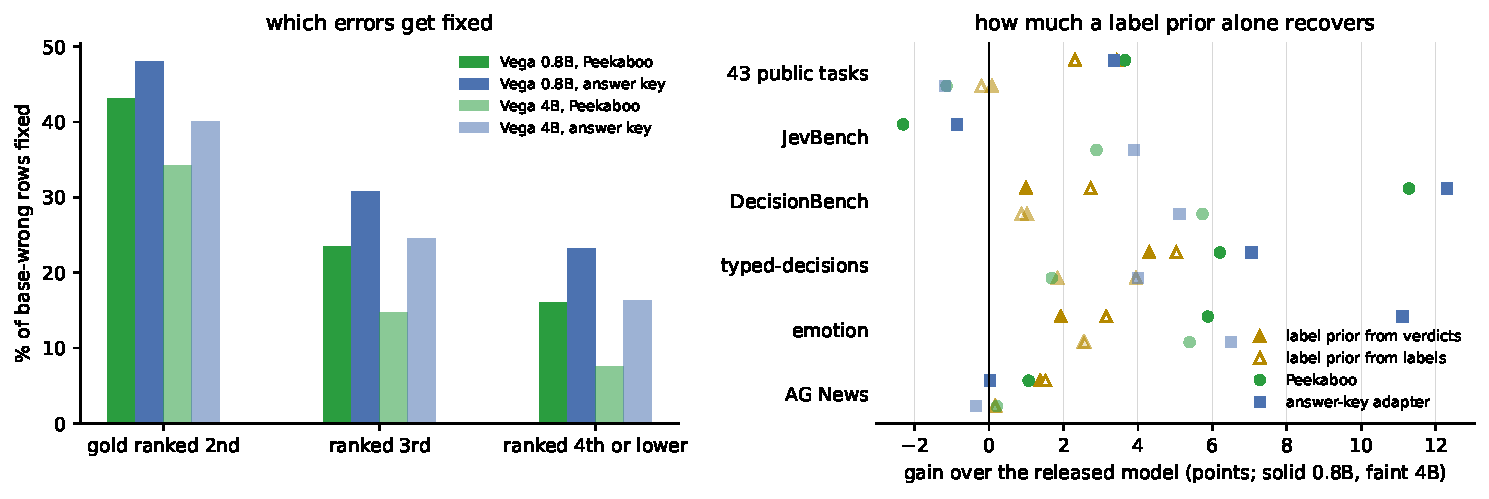
\includegraphics[width=\linewidth]{anatomy.pdf}
\caption{Left: share of the released model's wrong rows that eight-pass \pk{} and the answer-key adapter fix, by the released model's rank of the gold option (mean over benchmarks). Right: gain over the released model of a per-task label prior with no input features, trained from verdicts (filled triangles) or labels (open), beside \pk{} and the answer-key adapter.}
\label{fig:anatomy}
\end{figure}

\begin{table}[tbp]\centering\scriptsize
\caption{What the gain is made of. Left: gain over the released model of a per-task label prior with no input features (log-offsets on the released probabilities), trained from verdicts with Peekaboo's loop and from labels; and Peekaboo minus that prior. Right: how often eight on-policy passes reveal the gold answer: reward-1 events per training row (each one names the gold answer), the share of rows the base policy would reveal in 8 draws, the share of two-option rows, and the first pass's reward against the released model's best-answer accuracy on the same rows.}
\label{tab:anatomy}
\setlength{\tabcolsep}{2.5pt}
\resizebox{\linewidth}{!}{\begin{tabular}{llrrrr|rrrrr}
\toprule
model & benchmark & prior (verdicts) & prior (labels) & Peekaboo $-$ prior & params & reveals / row & $P$(revealed, 8 draws) & 2-option rows & pass-1 reward & base best-answer acc. \\
\midrule
Vega 0.8B & 43 public tasks & +3.4 & +2.3 & +0.2 {\scriptsize[-3.0, +3.1]} & 536 & 5.1 & 0.88 & 30\% & 0.50 & 0.55 \\
 & JevBench & -- & -- & -- & -- & 4.7 & -- & -- & 0.49 & -- \\
 & DecisionBench & +1.0 & +2.7 & +10.3 {\scriptsize[+6.3, +14.7]} & 28584 & 4.9 & 0.76 & 21\% & 0.48 & 0.50 \\
 & typed-decisions & +4.3 & +5.0 & +1.9 {\scriptsize[+0.1, +3.6]} & 71 & 6.1 & 0.94 & 30\% & 0.72 & 0.72 \\
 & emotion & +1.9 & +3.1 & +3.9 {\scriptsize[+2.1, +5.7]} & 6 & 4.9 & 0.85 & 0\% & 0.57 & 0.56 \\
 & AG News & +1.4 & +1.5 & -0.3 {\scriptsize[-1.2, +0.5]} & 4 & 7.5 & 0.97 & 0\% & 0.92 & 0.92 \\
\midrule
Vega 4B & 43 public tasks & +0.1 & -0.2 & -1.2 {\scriptsize[-3.6, +0.9]} & 536 & 6.1 & 0.92 & 30\% & 0.68 & 0.70 \\
 & JevBench & -- & -- & -- & -- & 5.9 & -- & -- & 0.64 & -- \\
 & DecisionBench & +1.0 & +0.9 & +4.7 {\scriptsize[+2.0, +7.8]} & 28584 & 5.6 & 0.82 & 21\% & 0.62 & 0.61 \\
 & typed-decisions & +1.8 & +3.9 & -0.2 {\scriptsize[-1.8, +1.6]} & 71 & 6.4 & 0.96 & 30\% & 0.75 & 0.79 \\
 & emotion & +2.5 & +2.6 & +2.9 {\scriptsize[+1.1, +4.7]} & 6 & 4.8 & 0.84 & 0\% & 0.57 & 0.57 \\
 & AG News & +0.2 & +0.2 & +0.0 {\scriptsize[-0.4, +0.6]} & 4 & 7.4 & 0.96 & 0\% & 0.92 & 0.93 \\
\midrule
Laya & typed-decisions & +15.3 & +17.4 & -- & 71 & -- & -- & -- & -- & -- \\
 & emotion & -1.4 & -3.3 & -- & 6 & -- & -- & -- & -- & -- \\
 & AG News & -0.6 & -0.1 & -- & 4 & -- & -- & -- & -- & -- \\
\bottomrule
\end{tabular}}
\end{table}

\begin{table}[tbp]\centering\small
\caption{Which rows change. Share of the released model's wrong rows that a method fixes, by the released model's rank of the gold option, and share of its right rows the method breaks (mean over benchmarks with a training split and over seeds).}
\label{tab:fixbreak}
\begin{tabular}{llrrrrr}
\toprule
model & method & fixed, all & gold 2nd & gold 3rd & gold 4th+ & broken \\
\midrule
Vega 0.8B & Peekaboo (8 passes) & 32\% & 43\% & 23\% & 13\% & 11\% \\
Vega 0.8B & Peekaboo (1 pass) & 26\% & 37\% & 13\% & 9\% & 8\% \\
Vega 0.8B & answer key (8 passes) & 40\% & 48\% & 31\% & 23\% & 13\% \\
Vega 4B & Peekaboo (8 passes) & 25\% & 34\% & 15\% & 8\% & 8\% \\
Vega 4B & Peekaboo (1 pass) & 18\% & 27\% & 9\% & 4\% & 6\% \\
Vega 4B & answer key (8 passes) & 32\% & 40\% & 25\% & 16\% & 10\% \\
Laya & Peekaboo (1 pass) & 0\% & 1\% & 0\% & 0\% & 0\% \\
Laya & Peekaboo, encoder (8) & 47\% & 58\% & 45\% & 32\% & 16\% \\
Laya & answer-key encoder (8) & 55\% & 65\% & 55\% & 44\% & 15\% \\
\bottomrule
\end{tabular}
\end{table}

\begin{table}[tbp]\centering\small
\caption{VegaML's TTT head answers a row only where a head was kept for its task and the option set matches (``covered''); elsewhere its output is the released engine's. Eight-pass Peekaboo minus TTT, and the answer-key adapter minus TTT, on covered and uncovered rows, under the vegaml 0.12.3 rule used in the main comparison; rows covered under the 0.8.0 rule for reference.}
\label{tab:ttt}
\resizebox{\linewidth}{!}{\begin{tabular}{llrrrrr}
\toprule
model & benchmark & covered (0.12.3) & covered (0.8.0) & Peekaboo $-$ TTT, covered & uncovered & answer key $-$ TTT, covered \\
\midrule
Vega 0.8B & 43 public tasks & 690 / 2535 & 1945 & -1.9 {\scriptsize[-8.6, +5.7]} & +3.0 {\scriptsize[-0.6, +6.9]} & -2.7 {\scriptsize[-8.3, +3.3]} \\
Vega 0.8B & DecisionBench & 329 / 1075 & 394 & +3.2 {\scriptsize[-2.0, +7.9]} & +11.5 {\scriptsize[+7.2, +16.1]} & +3.9 {\scriptsize[-1.3, +8.7]} \\
Vega 0.8B & typed-decisions & 600 / 2000 & 2000 & -0.7 {\scriptsize[-4.1, +2.8]} & +1.7 {\scriptsize[-0.2, +3.5]} & -0.4 {\scriptsize[-3.6, +2.9]} \\
Vega 0.8B & emotion & 1503 / 1503 & 1503 & -6.4 {\scriptsize[-8.4, -4.3]} & -- & -1.2 {\scriptsize[-3.3, +0.9]} \\
Vega 0.8B & AG News & 0 / 1912 & 1912 & -- & +1.1 {\scriptsize[+0.1, +2.0]} & -- \\
Vega 4B & 43 public tasks & 931 / 2535 & 2125 & -3.7 {\scriptsize[-8.5, +1.0]} & -0.6 {\scriptsize[-3.6, +2.4]} & -2.8 {\scriptsize[-6.9, +1.0]} \\
Vega 4B & DecisionBench & 302 / 1075 & 394 & +3.1 {\scriptsize[-1.9, +8.9]} & +4.3 {\scriptsize[+1.8, +7.1]} & +3.6 {\scriptsize[-1.9, +9.8]} \\
Vega 4B & typed-decisions & 600 / 2000 & 2000 & +1.7 {\scriptsize[-1.6, +5.1]} & -2.0 {\scriptsize[-4.4, +0.2]} & +2.7 {\scriptsize[-0.5, +6.0]} \\
Vega 4B & emotion & 1503 / 1503 & 1503 & -6.8 {\scriptsize[-8.9, -4.7]} & -- & -5.7 {\scriptsize[-7.7, -3.7]} \\
Vega 4B & AG News & 1912 / 1912 & 1912 & +1.5 {\scriptsize[+0.4, +2.6]} & -- & +1.0 {\scriptsize[-0.2, +2.1]} \\
\bottomrule
\end{tabular}}
\end{table}

\begin{table}[tbp]\centering\small
\caption{Benchmark artifacts. Gain over the released model with every task, and without the five tasks whose gold answer an adapter can learn without reading the input (public: truthfulqa\_mc1, pubmedqa; DecisionBench: contains\_threat, toxicity\_severity, finqa-numerical-reasoning).}
\label{tab:artifacts}
\resizebox{\linewidth}{!}{\begin{tabular}{llrrrr}
\toprule
model & method & public, all 43 & public, 41 tasks & DecisionBench, all 43 & DecisionBench, 40 tasks \\
\midrule
Vega 0.8B & Peekaboo (8) & +3.7 {\scriptsize[-0.1, +7.5]} & +1.9 {\scriptsize[-1.4, +5.1]} & +11.3 {\scriptsize[+7.0, +16.1]} & +9.3 {\scriptsize[+5.5, +14.0]} \\
Vega 0.8B & Peekaboo (1) & +1.9 {\scriptsize[-1.1, +5.2]} & +0.5 {\scriptsize[-2.1, +3.1]} & +6.7 {\scriptsize[+3.6, +10.5]} & +5.9 {\scriptsize[+2.8, +9.7]} \\
Vega 0.8B & answer key & +3.4 {\scriptsize[-0.9, +8.1]} & +1.5 {\scriptsize[-2.3, +5.3]} & +12.3 {\scriptsize[+7.8, +17.5]} & +10.2 {\scriptsize[+6.0, +15.1]} \\
Vega 0.8B & TTT (0.12.3) & +2.0 {\scriptsize[-0.8, +5.6]} & +1.0 {\scriptsize[-1.4, +3.5]} & +2.3 {\scriptsize[-1.3, +6.8]} & +1.3 {\scriptsize[-1.9, +5.5]} \\
Vega 4B & Peekaboo (8) & -1.1 {\scriptsize[-3.8, +1.5]} & -1.8 {\scriptsize[-4.5, +0.8]} & +5.7 {\scriptsize[+2.7, +9.3]} & +4.6 {\scriptsize[+2.1, +7.1]} \\
Vega 4B & Peekaboo (1) & +0.0 {\scriptsize[-2.9, +2.6]} & -0.4 {\scriptsize[-3.6, +2.1]} & +3.2 {\scriptsize[+1.5, +5.4]} & +3.4 {\scriptsize[+1.6, +5.7]} \\
Vega 4B & answer key & -1.2 {\scriptsize[-4.1, +1.8]} & -2.2 {\scriptsize[-5.0, +0.6]} & +5.1 {\scriptsize[+1.4, +9.1]} & +3.7 {\scriptsize[+0.5, +7.3]} \\
Vega 4B & TTT (0.12.3) & +0.6 {\scriptsize[-1.6, +3.0]} & +0.1 {\scriptsize[-2.1, +2.2]} & +1.8 {\scriptsize[-0.2, +4.2]} & +1.3 {\scriptsize[-0.6, +3.5]} \\
Laya & Peekaboo (1) & +0.1 {\scriptsize[-0.1, +0.3]} & +0.1 {\scriptsize[-0.1, +0.3]} & +0.1 {\scriptsize[+0.0, +0.3]} & +0.1 {\scriptsize[+0.0, +0.3]} \\
Laya & Peekaboo, encoder & +2.6 {\scriptsize[-0.8, +6.0]} & +2.0 {\scriptsize[-1.4, +5.5]} & +14.0 {\scriptsize[+8.8, +19.2]} & +12.9 {\scriptsize[+7.7, +18.1]} \\
Laya & their fine-tune & +1.0 {\scriptsize[-1.2, +3.5]} & +0.8 {\scriptsize[-1.6, +3.4]} & +3.1 {\scriptsize[-0.4, +7.3]} & +2.7 {\scriptsize[-1.1, +7.1]} \\
\bottomrule
\end{tabular}}
\end{table}


\paragraph{How much the protocol reveals.}
Table~\ref{tab:anatomy} (right) counts what eight on-policy passes tell the learner. On DecisionBench at 0.8B each training row produces $\revealsSmallPkDb$ reward-1 events on average, each of which names the gold answer; from the released model's own probabilities, 8 draws would hit the gold at least once on a share $\prevealSmallPkDb$ of the rows, and $\binarySmallPkDb$ of the rows have two options, where any verdict is the label. On typed-decisions the figures are $\revealsSmallPkTyped$ reveals per row and $\prevealSmallPkTyped$; on emotion $\revealsSmallPkEmo$ and $\prevealSmallPkEmo$. The first pass's reward, which is the only out-of-sample one, is $\passoneSmallPkDb$ on DecisionBench against the released model's best-answer accuracy of $\baseargmaxSmallPkDb$ on the same rows: the exploration a live system would pay for is a few points of accuracy during the first pass, and nothing afterwards if it then serves the argmax.

\paragraph{A label prior with no input.}
Per-task log-offsets on the released probabilities, one per (task, option text), trained with \pk{}'s own loop from verdicts, gain $\gainPriorFbSmallTyped$ on typed-decisions at 0.8B and $\gainPriorFbBigTyped$ at 4B, against \pk{}'s $\gainSmallPkTyped$ and $\gainBigPkTyped$; \pk{} minus the prior is $\gainPkVsPriorFbSmallTyped$ $\ciPkVsPriorFbSmallTyped$ and $\gainPkVsPriorFbBigTyped$ $\ciPkVsPriorFbBigTyped$. About two thirds of the typed-decisions gain at 0.8B, and all of it at 4B, is a prior shift that 71 numbers can learn from verdicts. On the public menu the prior gains $\gainPriorFbSmallPub$ and $\gainPriorFbBigPub$ (\pk{} minus prior $\gainPkVsPriorFbSmallPub$, $\gainPkVsPriorFbBigPub$). On DecisionBench the prior gains $\gainPriorFbSmallDb$ and $\gainPriorFbBigDb$ against \pk{}'s $\gainSmallPkDb$ and $\gainBigPkDb$, so there the adapter learns something the option text alone does not give (\pk{} minus prior $\gainPkVsPriorFbSmallDb$ $\ciPkVsPriorFbSmallDb$, $\gainPkVsPriorFbBigDb$ $\ciPkVsPriorFbBigDb$); on emotion the prior gains $\gainPriorFbSmallEmo$ and $\gainPriorFbBigEmo$ against $\gainSmallPkEmo$ and $\gainBigPkEmo$. DecisionBench and emotion are the benchmarks on which the paper's claim about learning from verdicts rests; typed-decisions and the public menu are largely prior correction, which verdicts also deliver, but which a 71-parameter model delivers too.

\paragraph{Which rows change.}
Table~\ref{tab:fixbreak} and Figure~\ref{fig:anatomy} (left) test the prediction of the $\pi(y)$ weighting. Over the benchmarks with a training split, eight-pass \pk{} fixes $\FixMeanSmallPk$\% of the released model's wrong rows at 0.8B and breaks $\BreakMeanSmallPk$\% of its right ones; the labelled adapter fixes $\FixMeanSmallSup$\% and breaks $\BreakMeanSmallSup$\%. Where the released model ranked the gold option second, \pk{} fixes $\FixRankTwoMeanSmallPk$\% of rows against the adapter's $\FixRankTwoMeanSmallSup$\%; where it ranked it fourth or lower, $\FixRankFourMeanSmallPk$\% against $\FixRankFourMeanSmallSup$\%. The verdict-trained adapter is the more conservative learner: it fixes fewer of the deep errors, as a $\pi(y)$-weighted objective must, and breaks fewer correct answers. The two differences partly offset each other, which is why the net accuracies are close; at DecisionBench's base accuracy the fixing deficit is the larger of the two.

\paragraph{Artifacts.}
Table~\ref{tab:artifacts} repeats the public-menu and DecisionBench gains without the five tasks whose gold answer can be learned from the option list alone (two on the public menu, three on DecisionBench). On the public menu at 0.8B \pk{}'s gain goes from $\gainSmallPkPub$ to $\gainSmallPkPubClean$ $\ciSmallPkPubClean$; at 4B from $\gainBigPkPub$ to $\gainBigPkPubClean$. On DecisionBench from $\gainSmallPkDb$ to $\gainSmallPkDbClean$ $\ciSmallPkDbClean$ and from $\gainBigPkDb$ to $\gainBigPkDbClean$ $\ciBigPkDbClean$. The labelled adapter and TTT profit from the same tasks, so the comparisons between methods move little; the gains over the released model are what the artifacts inflate. The per-task tables in Appendix~\ref{app:tasks} show where the rest of the DecisionBench gain sits.

\subsection{Calibration}
\label{sec:calibration}

\begin{figure}[t]\centering
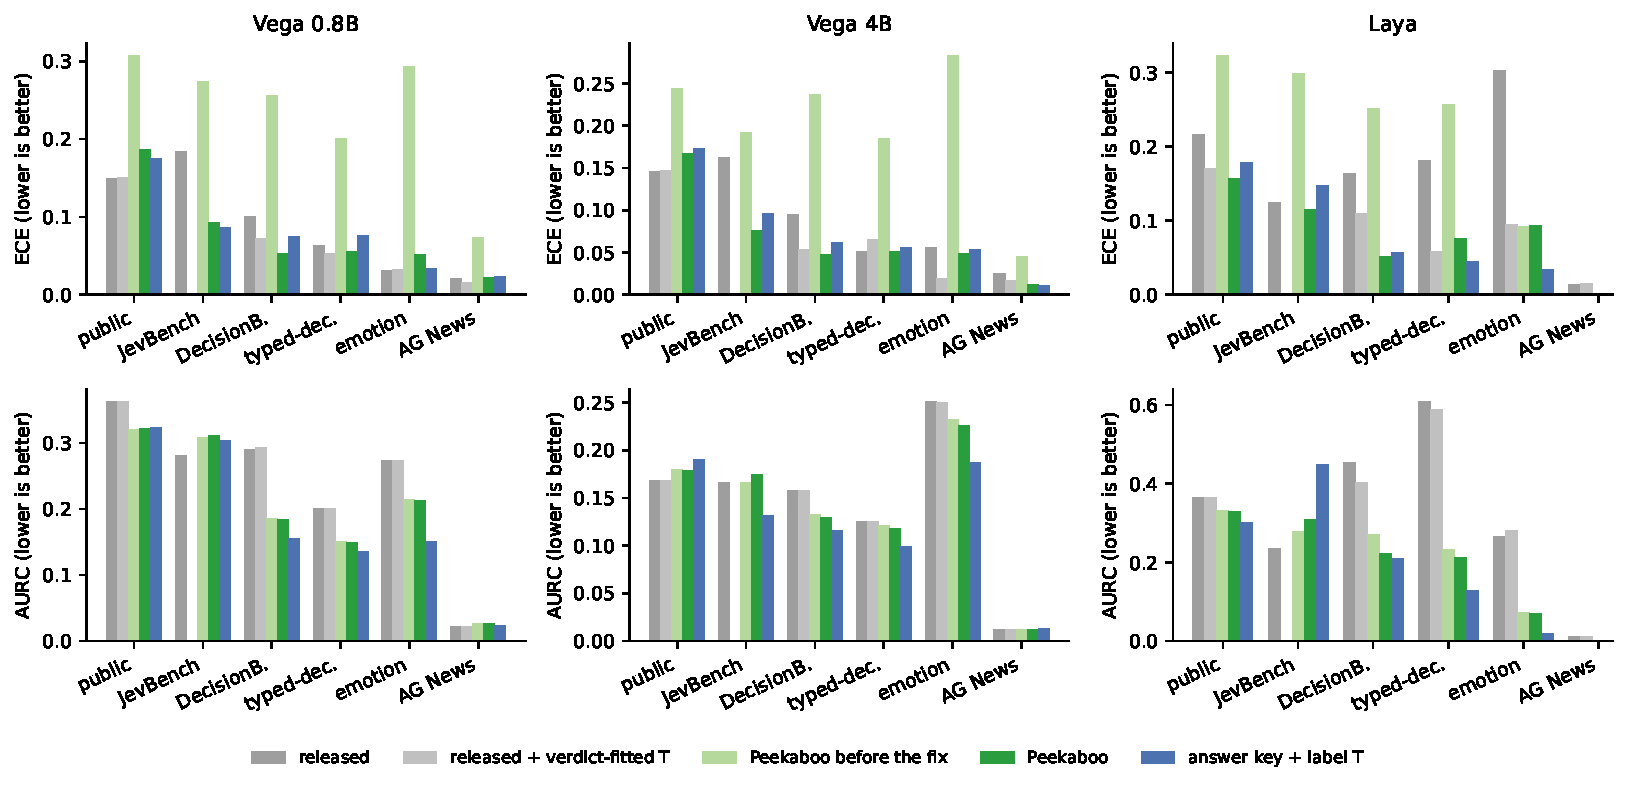
\includegraphics[width=\linewidth]{calibration.pdf}
\caption{ECE (top) and area under the risk-coverage curve (bottom), lower is better, for the released model, the released model with a temperature fitted from verdicts on its own calibration rows, \pk{} before and after the honesty fix, and the answer-key adapter with a label-fitted temperature. Laya: the encoder-unfrozen arms.}
\label{fig:cal}
\end{figure}

\begin{figure}[t]\centering
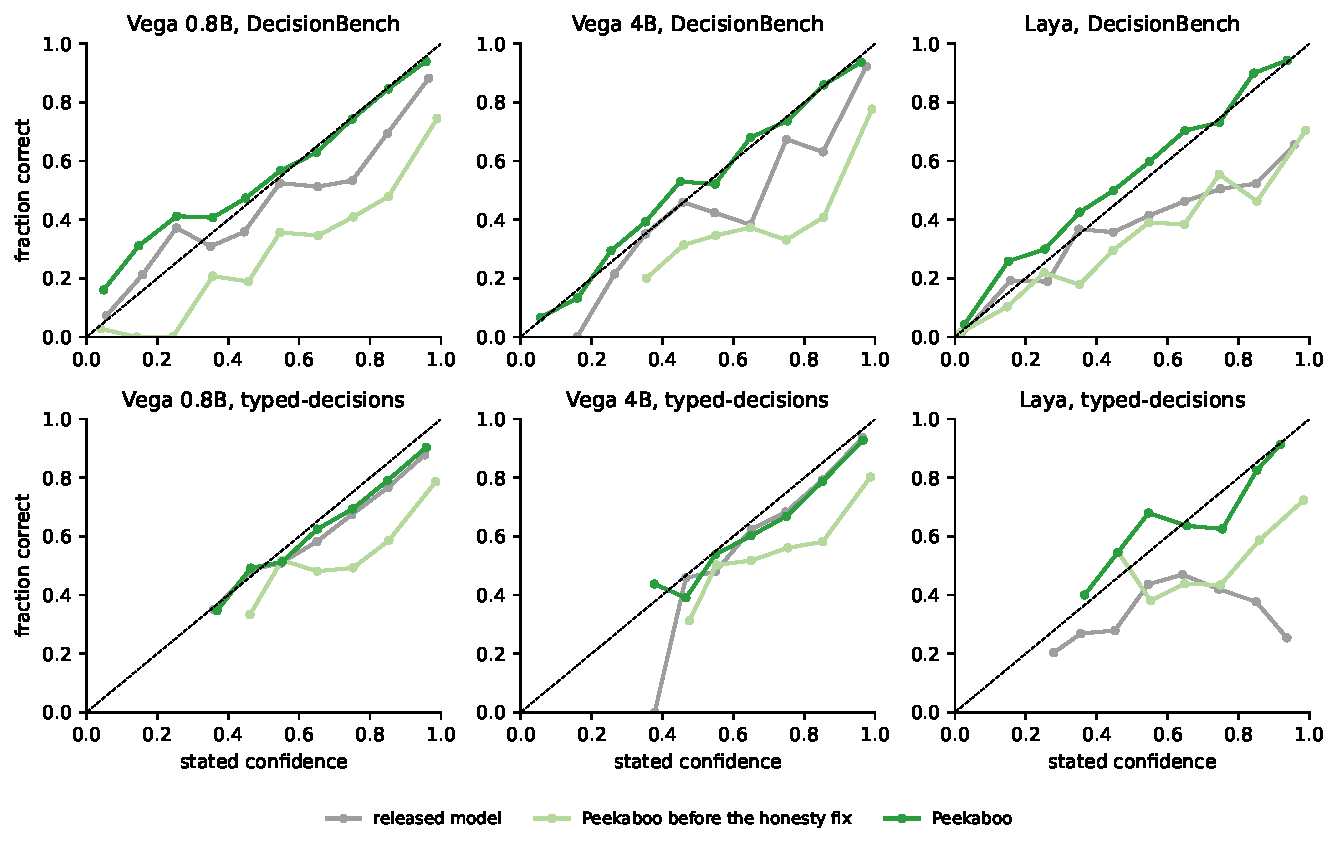
\includegraphics[width=0.9\linewidth]{reliability.pdf}
\caption{Reliability diagrams (10 bins on the confidence of the predicted option) on DecisionBench and typed-decisions: released model, \pk{} before the honesty fix, \pk{} after it (Laya: encoder unfrozen).}
\label{fig:rel}
\end{figure}

\begin{table}[tbp]\centering\scriptsize
\caption{Calibration and proper scores (lower is better; mean over seeds). ``+ T'' rows apply one temperature to the released model, fitted on its own calibration rows from verdicts on sampled answers (mean over 10 draws) or from labels.}
\label{tab:cal}
\setlength{\tabcolsep}{2.5pt}
\resizebox{\linewidth}{!}{\begin{tabular}{llrrrrrrrrrrrrrrrrrr}
\toprule
model & method & \multicolumn{3}{c}{public} & \multicolumn{3}{c}{JevBench} & \multicolumn{3}{c}{DecisionB.} & \multicolumn{3}{c}{typed-dec.} & \multicolumn{3}{c}{emotion} & \multicolumn{3}{c}{AG News} \\
 & & ECE & NLL & AURC & ECE & NLL & AURC & ECE & NLL & AURC & ECE & NLL & AURC & ECE & NLL & AURC & ECE & NLL & AURC \\
\midrule
\multicolumn{20}{l}{\textit{Vega 0.8B}} \\
 & released model & 0.150 & 1.100 & 0.363 & 0.184 & 1.262 & 0.281 & 0.101 & 1.631 & 0.291 & 0.063 & 0.753 & 0.200 & 0.031 & 1.193 & 0.274 & 0.021 & 0.291 & 0.023 \\
 & released + T from verdicts & 0.151 & 1.090 & 0.363 & -- & -- & -- & 0.072 & 1.509 & 0.294 & 0.053 & 0.747 & 0.200 & 0.033 & 1.192 & 0.274 & 0.016 & 0.289 & 0.023 \\
 & released + T from labels & 0.148 & 1.088 & 0.363 & -- & -- & -- & 0.089 & 1.515 & 0.296 & 0.050 & 0.745 & 0.201 & 0.036 & 1.191 & 0.274 & 0.016 & 0.289 & 0.023 \\
 & Peekaboo before the honesty fix & 0.308 & 2.735 & 0.321 & 0.275 & 1.758 & 0.308 & 0.257 & 3.547 & 0.186 & 0.200 & 1.354 & 0.151 & 0.293 & 3.593 & 0.215 & 0.073 & 0.707 & 0.026 \\
 & Peekaboo & 0.187 & 1.114 & 0.322 & 0.093 & 1.036 & 0.312 & 0.053 & 1.316 & 0.185 & 0.055 & 0.690 & 0.150 & 0.052 & 1.057 & 0.213 & 0.023 & 0.281 & 0.027 \\
 & Peekaboo, one pass & 0.177 & 1.102 & 0.342 & 0.079 & 1.006 & 0.287 & 0.059 & 1.376 & 0.212 & 0.059 & 0.714 & 0.160 & 0.046 & 1.045 & 0.211 & 0.012 & 0.256 & 0.020 \\
 & answer key + label temperature & 0.174 & 1.073 & 0.323 & 0.086 & 1.053 & 0.304 & 0.075 & 1.178 & 0.155 & 0.076 & 0.685 & 0.135 & 0.033 & 0.911 & 0.151 & 0.024 & 0.291 & 0.023 \\
\midrule
\multicolumn{20}{l}{\textit{Vega 4B}} \\
 & released model & 0.146 & 0.768 & 0.169 & 0.162 & 0.959 & 0.166 & 0.095 & 1.423 & 0.157 & 0.051 & 0.631 & 0.126 & 0.056 & 1.167 & 0.251 & 0.025 & 0.224 & 0.012 \\
 & released + T from verdicts & 0.147 & 0.761 & 0.169 & -- & -- & -- & 0.053 & 1.206 & 0.158 & 0.066 & 0.643 & 0.126 & 0.019 & 1.148 & 0.250 & 0.017 & 0.214 & 0.012 \\
 & released + T from labels & 0.153 & 0.764 & 0.169 & -- & -- & -- & 0.067 & 1.203 & 0.159 & 0.053 & 0.632 & 0.126 & 0.019 & 1.148 & 0.250 & 0.012 & 0.211 & 0.012 \\
 & Peekaboo before the honesty fix & 0.244 & 2.374 & 0.180 & 0.192 & 1.316 & 0.166 & 0.237 & 3.328 & 0.132 & 0.185 & 1.237 & 0.121 & 0.283 & 2.981 & 0.232 & 0.046 & 0.407 & 0.012 \\
 & Peekaboo & 0.167 & 0.836 & 0.179 & 0.076 & 0.783 & 0.174 & 0.047 & 1.095 & 0.129 & 0.051 & 0.637 & 0.118 & 0.049 & 1.087 & 0.226 & 0.012 & 0.208 & 0.012 \\
 & Peekaboo, one pass & 0.143 & 0.775 & 0.171 & 0.064 & 0.776 & 0.178 & 0.040 & 1.135 & 0.144 & 0.055 & 0.643 & 0.123 & 0.028 & 1.115 & 0.235 & 0.013 & 0.208 & 0.013 \\
 & answer key + label temperature & 0.173 & 0.840 & 0.191 & 0.096 & 0.679 & 0.131 & 0.062 & 1.051 & 0.116 & 0.056 & 0.567 & 0.100 & 0.054 & 0.996 & 0.187 & 0.011 & 0.220 & 0.013 \\
\midrule
\multicolumn{20}{l}{\textit{Laya}} \\
 & released model & 0.217 & 1.651 & 0.365 & 0.125 & 0.928 & 0.236 & 0.165 & 2.062 & 0.454 & 0.182 & 1.361 & 0.610 & 0.303 & 2.082 & 0.267 & 0.015 & 0.206 & 0.012 \\
 & released + T from verdicts & 0.171 & 1.189 & 0.365 & -- & -- & -- & 0.110 & 1.631 & 0.404 & 0.058 & 1.207 & 0.590 & 0.095 & 1.176 & 0.282 & 0.016 & 0.206 & 0.012 \\
 & released + T from labels & 0.174 & 1.159 & 0.361 & -- & -- & -- & 0.103 & 1.631 & 0.404 & 0.059 & 1.205 & 0.588 & 0.097 & 1.177 & 0.282 & 0.017 & 0.206 & 0.012 \\
 & Peekaboo, one pass & 0.163 & 1.111 & 0.364 & 0.107 & 0.911 & 0.245 & 0.075 & 1.575 & 0.389 & 0.034 & 1.194 & 0.563 & -- & -- & -- & -- & -- & -- \\
 & Peekaboo, encoder unfrozen & 0.157 & 1.088 & 0.329 & 0.115 & 1.024 & 0.309 & 0.052 & 1.392 & 0.223 & 0.077 & 0.827 & 0.213 & 0.094 & 0.665 & 0.070 & -- & -- & -- \\
 & answer-key encoder + label temperature & 0.179 & 1.025 & 0.303 & 0.148 & 1.085 & 0.448 & 0.057 & 1.296 & 0.211 & 0.045 & 0.636 & 0.129 & 0.035 & 0.313 & 0.018 & -- & -- & -- \\
\bottomrule
\end{tabular}}
\end{table}


Before the honesty fix the trained add-on is badly over-confident: ECE $\eceSmallPkRawDb$ on DecisionBench at 0.8B, $\eceBigPkRawDb$ at 4B, $\eceSmallPkRawEmo$ and $\eceBigPkRawEmo$ on emotion (Table~\ref{tab:cal}, Figure~\ref{fig:rel}). One temperature fitted from verdicts brings these to $\eceSmallPkDb$, $\eceBigPkDb$, $\eceSmallPkEmo$ and $\eceBigPkEmo$. Against the released model the picture is mixed. \pk{}'s ECE is lower on DecisionBench and JevBench at both sizes, on typed-decisions at 0.8B and on emotion and AG News at 4B, and higher on the public menu at both sizes and on emotion and AG News at 0.8B (Table~\ref{tab:cal}). The control the first version lacked, the released model with the same temperature fitted on its own calibration rows, reaches $\eceBaseTFbSmallDb$ and $\eceBaseTFbBigDb$ on DecisionBench against the released model's $\eceSmallBaseDb$ and $\eceBigBaseDb$; \pk{} is better calibrated than this control in four of the ten Vega cells where both exist (DecisionBench at both sizes, typed-decisions and AG News at 4B) and worse in the other six. Much of the ECE improvement the first version credited to the adapter is the temperature. On proper scores the adapter does help: its Brier score is below the released model's on every Vega benchmark but the public menu at 4B, and on DecisionBench at 0.8B its NLL is $\nllSmallPkDb$ against the released model's $\nllSmallBaseDb$, though above the labelled adapter's $\nllSmallSupDb$. Selective risk (AURC), which depends almost only on how rows are ranked by confidence, is better than the released model's on DecisionBench, typed-decisions and emotion at both sizes and on the public menu at 0.8B, and worse on JevBench at both sizes, on the public menu at 4B and on AG News at 0.8B (Figure~\ref{fig:cal}). The fitted temperatures range from $\Tmin$ to $\Tmax$ with a median of $\Tmedian$ (Figure~\ref{fig:switch_T}); part of each is inherited from the released model, which itself prefers a temperature above 1 on most benchmarks ($\TBaseTFbSmallDb$ on DecisionBench at 0.8B).

\subsection{The KL term and the switch}
\label{sec:ablation}

\begin{figure}[t]\centering
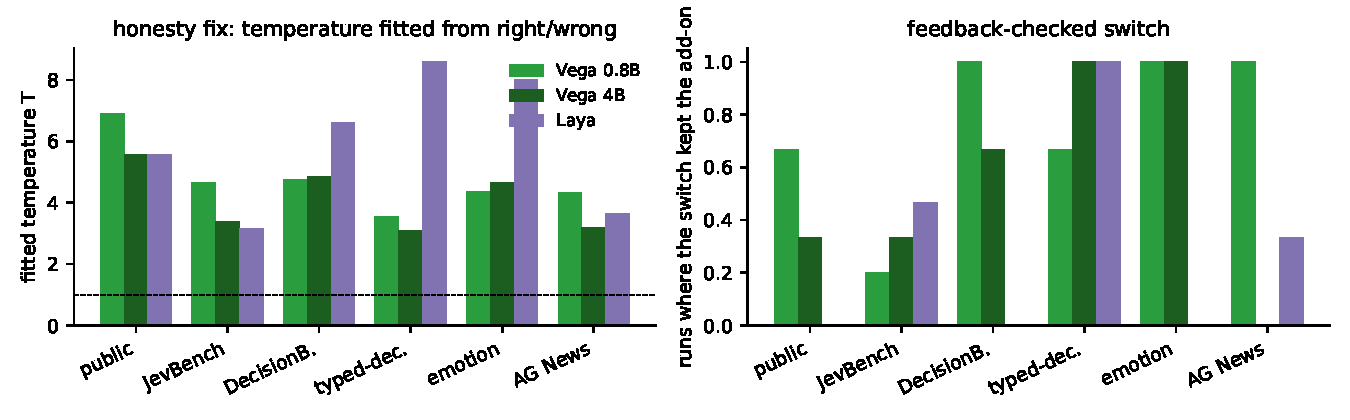
\includegraphics[width=0.9\linewidth]{switch_T.pdf}
\caption{Left: the temperature fitted from verdicts per model and benchmark (dashed line at $T = 1$; Laya: encoder unfrozen). Right: the share of runs in which the switch, comparing best answers on the calibration rows, kept the add-on; black ticks show the first version's switch on the same runs, which compared sampled answers.}
\label{fig:switch_T}
\end{figure}

Removing the KL term changes eight-pass \pk{} by $\gainSmallPkDbVsKlzero$ $\ciSmallPkDbVsKlzero$ points on DecisionBench at 0.8B and $\gainBigPkDbVsKlzero$ $\ciBigPkDbVsKlzero$ at 4B (positive means the term helps; Table~\ref{tab:h2h}), $\gainSmallPkTypedVsKlzero$ and $\gainBigPkTypedVsKlzero$ on typed-decisions, $\gainSmallPkPubVsKlzero$ and $\gainBigPkPubVsKlzero$ on the public menu, and $\gainSmallPkEmoVsKlzero$ and $\gainBigPkEmoVsKlzero$ $\ciBigPkEmoVsKlzero$ on emotion. The term is decisive in one cell, emotion at 4B, where the run without it collapsed, and that is the only KL contrast that survives Holm adjustment; elsewhere it is worth between $-0.6$ and $+2.2$ points and none of those differences survives. The no-KL arm has three seeds on DecisionBench and on JevBench at 0.8B, and one elsewhere. The first version's ``where the method lives'' was too strong.

The switch now compares best answers, which takes two verdicts on the same question, one of them on an answer the system did not serve; a deployment would have to run it as a held-out comparison on a slice of traffic. At 0.8B it turns the add-on off on JevBench, where \pk{} loses $\absSmallPkJev$ points (gain with the switch $\gainSmallPkSwJev$), and keeps it on every other benchmark. At 4B it keeps the add-on on DecisionBench and emotion; it also keeps it on the public menu, where \pk{} is $\gainBigPkPub$ (not significant), and it drops it in most JevBench folds and on typed-decisions, giving up gains of $\gainBigPkJev$ and $\gainBigPkTyped$ that were themselves not significant. The first version's switch, computed on the same runs, kept the add-on in $\swOnSampledBigPkDb$\% of the DecisionBench runs at 4B, where the new one keeps it in $\swOnBigPkDb$\%; the two statistics disagree in the direction Section~\ref{sec:switch} describes.

\subsection{Laya: head, encoder, and the matched fine-tune}
\label{sec:laya}

\begin{figure}[t]\centering
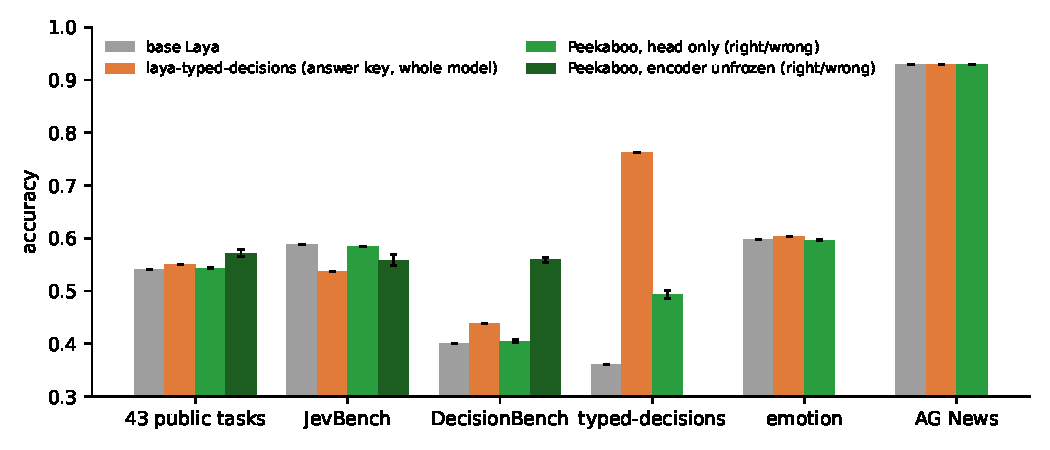
\includegraphics[width=0.85\linewidth]{laya.pdf}
\caption{Laya with the encoder unfrozen: gain over released Laya of the typed-decisions fine-tune (in-domain only on typed-decisions), the matched answer-key fine-tune (same rows, passes and KL term, early-stopped), \pk{} with eight passes and with one pass, and head-only \pk{} with one pass. Encoder arms have three seeds on the public menu and JevBench, two on DecisionBench and one on typed-decisions and emotion; AG News was not run.}
\label{fig:laya}
\end{figure}

With the encoder frozen, a trainable copy of Laya's head learns a prior shift and little else; in the first version's grid, eight passes gave $\gainVoneLayaPkTyped$ points on typed-decisions where a 71-offset prior from the same verdicts gave $\gainVonePriorFbLayaTyped$, and in this grid one pass gives $\gainLayaPkOneTyped$. With the encoder unfrozen, verdicts move the whole model: $\gainLayaPkEncTyped$ $\ciLayaPkEncTyped$ on typed-decisions with eight passes, $\gainLayaPkEncOneTyped$ with one, $\gainLayaPkEncEmo$ on emotion, $\gainLayaPkEncDb$ on DecisionBench and $\gainLayaPkEncPub$ on the public menu. The comparison the first version lacked is the same fine-tune on labels: cross-entropy, same rows, passes and KL term, encoder unfrozen. It gains $\gainLayaSupEncTyped$ on typed-decisions, $\gainLayaSupEncEmo$ on emotion, $\gainLayaSupEncDb$ on DecisionBench and $\gainLayaSupEncPub$ on the public menu; \pk{} minus this arm is $\gainLayaPkEncTypedVsSupEnc$ $\ciLayaPkEncTypedVsSupEnc$ on typed-decisions, $\gainLayaPkEncEmoVsSupEnc$ $\ciLayaPkEncEmoVsSupEnc$ on emotion, $\gainLayaPkEncDbVsSupEnc$ on DecisionBench and $\gainLayaPkEncPubVsSupEnc$ on the public menu. At matched capacity and data, labels beat eight rounds of verdicts clearly on typed-decisions and emotion. On DecisionBench and the public menu the gap is one to two points and within the noise. On JevBench the two are level: \pk{} minus the same-recipe arm is $\gainLayaPkEncJevVsSupEnc$ $\ciLayaPkEncJevVsSupEnc$ and minus the early-stopped one $\gainLayaPkEncJevVsSupEncEs$ $\ciLayaPkEncJevVsSupEncEs$. One pass costs the encoder arm a lot ($\gainLayaPkEncOneTypedVsPkEnc$ on typed-decisions, $\gainLayaPkEncOneEmoVsPkEnc$ on emotion against eight passes); no one-pass labelled encoder arm was run, so these have no matched label comparator. The head-only one-pass arm barely moves from the released model ($\gainLayaPkOneTyped$ on typed-decisions) where the one-pass labelled head gains $\gainLayaSupOneTyped$.
On typed-decisions the matched fine-tune reaches $\accLayaSupEncTyped$ against the released \texttt{laya-typed-decisions} checkpoint's $\accLayaTdTyped$, so our labelled arm is a fair stand-in for Laya's own recipe. Away from typed-decisions the released fine-tune is a transfer model that never saw the benchmark, and in-domain training of any kind beats it: \pk{} with the encoder is $\gainLayaPkEncEmoVsTd$ above it on emotion and $\gainLayaPkEncDbVsTd$ on DecisionBench, the labelled encoder arm $\gainLayaSupEncEmoVsTd$ and $\gainLayaSupEncDbVsTd$. Those numbers say that fine-tuning on a benchmark's own rows helps on that benchmark; they say nothing about verdicts against labels, and we do not use them to.

\subsection{typed-decisions without Vega's shipped adapter}
\label{sec:noship}
\begin{table}[tbp]\centering\small
\caption{typed-decisions on Vega with the shipped \texttt{typed\_decisions} adapter, which was fitted with labels on this feedback pool, switched off. Accuracy (mean over seeds) and gain over the corresponding released model.}
\label{tab:noship}
\resizebox{\linewidth}{!}{\begin{tabular}{llrrrr}
\toprule
model & method & accuracy, adapters on & gain & accuracy, adapters off & gain \\
\midrule
Vega 0.8B & released engine & 0.666 & -- & 0.377 & -- \\
Vega 0.8B & answer-key adapter (8) & 0.737 {\scriptsize$\pm$0.002} & +7.0 {\scriptsize[+5.0, +9.1]} & 0.693 {\scriptsize$\pm$0.013} & +31.6 {\scriptsize[+28.9, +34.4]} \\
Vega 0.8B & Peekaboo (8) & 0.728 {\scriptsize$\pm$0.007} & +6.2 {\scriptsize[+4.2, +8.2]} & 0.507 {\scriptsize$\pm$0.028} & +13.0 {\scriptsize[+9.8, +16.5]} \\
Vega 0.8B & Peekaboo (1) & 0.708 {\scriptsize$\pm$0.003} & +4.1 {\scriptsize[+2.2, +6.1]} & 0.498 {\scriptsize$\pm$0.007} & +12.1 {\scriptsize[+10.1, +14.2]} \\
Vega 4B & released engine & 0.729 & -- & 0.440 & -- \\
Vega 4B & answer-key adapter (8) & 0.769 {\scriptsize$\pm$0.001} & +4.0 {\scriptsize[+2.5, +5.6]} & 0.748 {\scriptsize$\pm$0.006} & +30.8 {\scriptsize[+27.8, +33.9]} \\
Vega 4B & Peekaboo (8) & 0.746 {\scriptsize$\pm$0.010} & +1.7 {\scriptsize[-0.1, +3.6]} & 0.685 {\scriptsize$\pm$0.027} & +24.6 {\scriptsize[+21.0, +28.5]} \\
Vega 4B & Peekaboo (1) & 0.749 {\scriptsize$\pm$0.004} & +2.0 {\scriptsize[+0.7, +3.5]} & 0.661 {\scriptsize$\pm$0.004} & +22.2 {\scriptsize[+19.4, +25.0]} \\
\bottomrule
\end{tabular}}
\end{table}

Vega's released \texttt{typed\_decisions} adapter was fitted on the pool our methods learn from, so on this benchmark ``released Vega'' already carries those labels. With the shipped adapters switched off the released engine scores $\accSmallNoshipBaseTyped$ at 0.8B and $\accBigNoshipBaseTyped$ at 4B (Table~\ref{tab:noship}). From that start eight-pass \pk{} gains $\gainSmallPkNoshipTypedVsNoshipBase$ $\ciSmallPkNoshipTypedVsNoshipBase$ and $\gainBigPkNoshipTypedVsNoshipBase$ $\ciBigPkNoshipTypedVsNoshipBase$, the labelled adapter $\gainSmallSupNoshipTypedVsNoshipBase$ and $\gainBigSupNoshipTypedVsNoshipBase$, and one-pass \pk{} $\gainSmallPkOneNoshipTypedVsNoshipBase$ and $\gainBigPkOneNoshipTypedVsNoshipBase$. The gap between verdicts and labels, $\gainSmallPkNoshipTypedVsSupNoship$ at 0.8B and $\gainBigPkNoshipTypedVsSupNoship$ at 4B, is far wider than with the shipped adapter on, which is the clearest demonstration in the paper of what the $\pi(y)$ weighting means: when the released model puts little probability on the gold answer, a verdict on a sampled answer rarely finds it, and labels do.


\section{Limitations}
\label{sec:limitations}
\begin{itemize}
\item \textbf{Verdicts come from gold answers.} Flipped, missing and complaint-skewed verdicts are simulated; a rater who is systematically wrong about what was right is not, and real deployments (Kreutzer et al.~\citep{kreutzer2018ebay}; Gao et al.~\citep{gao2023continually}) find explicit ratings noisier than this.
\item \textbf{Seeds.} The eight-pass, one-pass and answer-key arms have three seeds everywhere. Because one Laya encoder run takes about twenty minutes on the GPU we could afford, the encoder arms have three seeds on the public menu and JevBench, two on DecisionBench and one on typed-decisions and emotion, and none on AG News; the realistic-feedback and no-KL arms have three seeds on DecisionBench and one elsewhere, and were run on Vega only; the Laya head-only arms were run for one pass (three seeds on typed-decisions, one on the public menu and DecisionBench); the Laya head-only eight-pass arms are taken from the first version's grid, where the labelled head had no KL term. Single-seed intervals carry row and cluster resampling only.
\item \textbf{Two released models, four vendor benchmarks.} Vega and Laya are both from one developer and neither has a paper; JevBench and DecisionBench are small and recent. Emotion and AG News are the only standard sets, and on AG News the released models are already at 0.93.
\item \textbf{Benchmark artifacts and contamination.} Four tasks have learnable gold positions or option structures; Vega's shipped adapter was fitted on the typed-decisions pool; the engines' training corpora are undisclosed, so overlap with the public menu cannot be ruled out. We report around these, not without them.
\item \textbf{Hyper-parameters.} $\beta$, the rank, the learning rates and the eight passes were fixed before this grid, $\beta$ in a pilot that used DecisionBench test rows. The labelled arms were tuned only by early stopping on calibration labels; the verdict arms not at all.
\item \textbf{One temperature per benchmark.} On the 43-task public menu this is too coarse, and ECE there is mostly small-sample estimator bias; a per-task temperature fitted the same way is the obvious next step.
\item \textbf{Same-seed reruns differ.} Across machines a single run moves by up to 3 points; conclusions should rest on the three-seed means and the intervals, not on single cells.
\end{itemize}


\section{Conclusion}
The question we set out to answer was how much of a decision model's labelled-data recipe right / wrong feedback recovers. Under repeated on-policy feedback the answer is most of it, because repeated verdicts on the same rows are largely labels in disguise and the update is a reweighted cross-entropy. With one rating per row, which is what a deployment collects, it is less: on DecisionBench one on-policy pass keeps $\gainSmallPkOneDb$ of the eight-pass $\gainSmallPkDb$ at 0.8B, and one logged verdict per row trained to convergence $\gainSmallLogIpsDb$, and every one-rating arm below the labels but one, where it is level. The gain depends on the released model already putting the right answer near the top; with Vega's shipped typed-decisions adapter switched off, labels gain $\gainSmallSupNoshipTypedVsNoshipBase$ points and eight passes of verdicts $\gainSmallPkNoshipTypedVsNoshipBase$. On typed-decisions and the public menu much of what verdicts deliver is a label prior that a few dozen numbers could learn; on DecisionBench and emotion it is not. On Laya the matched fine-tune on labels wins where the gap is measurable. None of the parts is new; the measurement is, and so is the list of things that made the first version's numbers look better than they were. The next experiment is the one this grid cannot run: a model deployed with real users, their verdicts logged once on the answer it actually gave, with noise that comes from people rather than from a coin.


\paragraph{Acknowledgements.}
We thank the authors of VegaML and Laya for releasing their models, benchmark code and training recipes, and the reviewers of the first version, whose report is reproduced in the repository.

\FloatBarrier
\bibliographystyle{plainnat}
\bibliography{refs}

\appendix
\section{What the review found, and what changed}
\label{app:changes}
The first version of this paper (repository commit \texttt{cd52a9f}) was reviewed by a panel of thirteen automated specialist reviewers with an independent verifier for every major finding; the full report, its per-row scripts and its verdicts are in the repository under \texttt{reports/critique.zip}. Every number it quotes reproduced from our records, and it found no test-set leakage and no cherry-picked reruns. Its objections were to what was compared with what, and to what was claimed. Table~\ref{tab:changes} lists each major finding and what this version does about it.

\begin{table}[H]\centering\scriptsize
\caption{The review's major findings and this version's response.}
\label{tab:changes}
\setlength{\tabcolsep}{4pt}
\begin{tabular}{p{5.6cm}p{9.6cm}}
\toprule
finding & response \\
\midrule
``One bit per row'' misdescribed the protocol: eight on-policy passes rate each row up to eight times and reveal the gold answer for most rows. & Every feedback arm now has a one-pass version in which each row is rated once; the one-pass number is reported as the deployment figure. Reveal statistics are measured and reported (Table~\ref{tab:anatomy}). The ``$\log_2 k$ bits against one'' argument is gone. \\
The expected update of REINFORCE with a 0/1 reward is cross-entropy weighted by $\pi(y)$; the gains are a known effect. & Stated in Section~\ref{sec:method} and cited; the fix / break analysis by gold rank tests the prediction (Table~\ref{tab:fixbreak}). The paper no longer claims a new learning setting. \\
The switch compared sampled answers, so it measured expected gold probability, not deployed accuracy; it threw away real gains on 641- and 1,200-row calibration sets and kept a loss on emotion. & The switch compares best answers (two verdicts per row). The old statistic is still computed and shown beside it (Figure~\ref{fig:switch_T}). \\
Laya with the encoder unfrozen was compared with a fine-tune that never saw the benchmark; the matched answer-key encoder fine-tune had been dropped. & The matched arm (\texttt{sup\_enc}: same rows, passes, KL term, encoder unfrozen) is run on every benchmark, with and without early stopping. \texttt{laya-typed-decisions} is presented as in-domain only on typed-decisions. \\
Laya's answer-key head was trained without the KL term the paper described. & It now has the same KL term as Vega's adapter. \\
The answer-key adapter was called an upper bound but was untuned and over-trained by epoch 8. & An early-stopped version (epoch chosen on the calibration rows' labels) is reported next to the same-recipe version; neither is called an upper bound. \\
Win counts counted statistical ties and used six as the denominator where TTT is defined on five benchmarks; the answer-key arms were not run on JevBench. & Counts are by Holm-adjusted significance within a family, out of the benchmarks where the comparison exists; every answer-key arm is cross-fitted on JevBench. \\
Intervals ignored seed variance; the KL ablation had none. & All intervals resample seeds and row clusters; $p$-values are Holm-adjusted; the KL contrasts carry intervals. \\
More than half of the 0.8B public-menu gain came from truthfulqa\_mc1 (gold always first) and pubmedqa (majority class); about a quarter of the DecisionBench gain from two artifact tasks. & Disclosed in Section~\ref{sec:setup}; every public and DecisionBench number is reported with and without those tasks (Table~\ref{tab:artifacts}); per-task tables for both. \\
A per-task label prior with no features reproduces the typed-decisions gains and part of the others. & The prior baseline is run from verdicts and from labels on every benchmark (Table~\ref{tab:anatomy}, Figure~\ref{fig:anatomy}). \\
Vega's shipped typed\_decisions adapter was fitted on the typed-decisions feedback pool. & Disclosed; typed-decisions on Vega is also run with the shipped adapters off (Table~\ref{tab:noship}). \\
The feedback pools were class-balanced against naturally distributed test sets (emotion, public). & Emotion and AG News pools are now random draws with the natural class mix; the public pool is VegaML's protocol and is described as such. \\
The ECE comparison with the base model credited temperature scaling to the adapter; calibration was reported as ECE only. & The released model with the same verdict-fitted temperature (and a label-fitted one) is a reported control; NLL, Brier and AURC appear beside ECE (Table~\ref{tab:cal}). \\
TTT was scored under vegaml 0.8.0's rule; 0.12.3 requires the head to beat the engine as well. & Both rules are reported. \\
The honesty fix is standard top-label temperature scaling from correctness bits; over-sharpening after policy gradient is known. & Positioned as such in Sections~\ref{sec:method} and Related work. \\
The no-engine control used an entropy bonus, not the KL term the paper said, and sat at chance. & Dropped from the paper. \\
$\beta$ was chosen on DecisionBench test rows; $\beta=1$ runs were unreported; the KL pilot did not fully reproduce. & Disclosed in Section~\ref{sec:method} and below. \\
The reward curve was presented as a bound on live exploration cost; passes 2--8 are in-sample. & Replaced by the pass-1 reward against the released model's best-answer accuracy on the same rows (Table~\ref{tab:anatomy}). \\
Many prose numbers were hard-coded and several contradicted the tables. & Every number in the text is a macro generated from the records. \\
The encoder-unfrozen variant was added after the grid was called final. & All arms were run in one grid for this version. \\
\bottomrule
\end{tabular}
\end{table}

\paragraph{The $\beta$ pilot.} $\beta=0.1$ was chosen in October 2026 from $\{0, 0.1, 1\}$ in a pilot on DecisionBench that trained on 645 and tested on 430 of the README's 1,075 test rows, and in a learning-curve study whose test set overlapped the README slice. In that pilot $\beta=1$ kept about 80\% of the gain at 0.8B; in the learning-curve study it kept about a third. The first version's grid also ran $\beta=1$ on the public menu and JevBench at 0.8B without reporting it: $\beta=1$ scored 0.584 against 0.590 for $\beta=0.1$ on the public menu and 0.548 against 0.517 on JevBench (released model 0.550). An independent reproduction of the first version's DecisionBench study on another machine recovered the headline gain ($+10.4$ against $+10.2$) but not the KL pilot's gap ($\beta=0$: 0.566 against 0.571 for $\beta=0.1$, where the pilot had 0.536 against 0.567). None of this was retuned for this version; $\beta=0.1$ is used throughout and the no-KL ablation has intervals.

\section{Reproducing the results}
\label{app:repro}
\texttt{experiments/peekaboo\_remaining/run.py --grid v2} runs the whole grid: it reads every benchmark once through every model and caches the backbone features and the official records, replays each released model against its official prediction call, then runs every method and seed and writes \texttt{output\_v2/TABLES.md}. Finished steps are skipped, so the run can be resumed. \texttt{analysis.py} computes every interval, control and statistic in this paper from the per-row records, and \texttt{paper/make\_figures.py} produces every table, figure and number macro. The first version's grid (\texttt{--grid v1}) and its results under \texttt{output/} are kept for comparison; its DecisionBench learning-curve study is \texttt{experiments/vega\_policy/reproduce.py}.

\paragraph{Checks.} Replaying each released model on its cached inputs matches the official prediction call to $0$ for Vega and to $5\times10^{-5}$ for Laya (one question per forward pass, as Laya's own call runs it). The released models reproduce their README figures: Vega 0.8B and 4B on the public menu at $\accSmallBasePub$ and $\accBigBasePub$ against the README's 0.556 and 0.717, DecisionBench at $\accSmallBaseDb$ and $\accBigBaseDb$ against 0.509 and 0.633; Laya and laya-typed-decisions on typed-decisions at $\accLayaBaseTyped$ and $\accLayaTdTyped$ against 0.362 and 0.766. Results on the same seed differ across machines by up to 3 points for a single run (floating-point non-determinism in feature extraction and training kernels); the three-seed means are what reproduce.

\section{Per-task results}
\label{app:tasks}
\begin{table}[tbp]\centering\scriptsize
\caption{Accuracy on each of the 43 public tasks (mean over seeds). key: the early-stopped answer-key adapter / head; Pk8, Pk1: Peekaboo with eight passes, one pass; f-t: laya-typed-decisions; -enc: encoder unfrozen. $^*$ marks the two tasks with a construction artifact. Bold: the best method for that model on that task.}
\label{tab:tasks}
\setlength{\tabcolsep}{2pt}
\resizebox{\linewidth}{!}{\begin{tabular}{lrrrrrrrrrrrrrr}
\toprule
task & \multicolumn{5}{c}{Vega 0.8B} & \multicolumn{5}{c}{Vega 4B} & \multicolumn{4}{c}{Laya} \\
 & base & TTT & key & Pk8 & Pk1 & base & TTT & key & Pk8 & Pk1 & base & f-t & key-enc & Pk-enc \\
\midrule
aegis\_prompt\_safety & 0.50 & 0.50 & 0.64 & \textbf{0.64} & 0.57 & 0.60 & 0.60 & \textbf{0.79} & 0.74 & 0.73 & 0.37 & 0.43 & 0.68 & \textbf{0.70} \\
ag\_news & \textbf{0.97} & \textbf{0.97} & \textbf{0.97} & \textbf{0.97} & \textbf{0.97} & 0.95 & 0.95 & \textbf{0.97} & 0.95 & 0.97 & \textbf{0.98} & \textbf{0.98} & 0.97 & 0.97 \\
anli\_r3 & 0.28 & 0.28 & \textbf{0.39} & 0.37 & 0.32 & 0.35 & \textbf{0.52} & 0.43 & 0.40 & 0.39 & \textbf{0.43} & 0.40 & 0.42 & 0.42 \\
arc\_challenge & 0.48 & 0.48 & 0.44 & \textbf{0.50} & 0.48 & 0.80 & 0.80 & 0.80 & 0.81 & \textbf{0.83} & 0.28 & \textbf{0.37} & 0.34 & \textbf{0.37} \\
arc\_easy & \textbf{0.60} & \textbf{0.60} & 0.55 & 0.55 & 0.58 & 0.92 & 0.92 & \textbf{0.95} & 0.94 & 0.93 & 0.52 & 0.57 & \textbf{0.57} & 0.57 \\
banking77 & 0.68 & 0.68 & \textbf{0.72} & 0.66 & 0.62 & 0.73 & 0.73 & \textbf{0.74} & 0.69 & 0.69 & 0.42 & 0.40 & \textbf{0.48} & 0.37 \\
boolq & 0.75 & 0.75 & 0.76 & \textbf{0.82} & 0.79 & 0.82 & 0.82 & 0.84 & 0.84 & \textbf{0.91} & \textbf{0.87} & 0.85 & 0.78 & 0.83 \\
casehold & 0.35 & 0.35 & \textbf{0.49} & 0.46 & 0.42 & 0.55 & 0.55 & \textbf{0.63} & 0.61 & 0.63 & 0.38 & 0.38 & 0.38 & \textbf{0.45} \\
climate\_fever & 0.35 & 0.38 & \textbf{0.47} & 0.38 & 0.36 & 0.45 & 0.38 & \textbf{0.48} & 0.46 & \textbf{0.48} & 0.33 & \textbf{0.35} & 0.25 & 0.30 \\
clinc150\_oos & \textbf{0.68} & \textbf{0.68} & 0.62 & 0.62 & 0.61 & \textbf{0.92} & \textbf{0.92} & 0.83 & 0.78 & 0.83 & 0.00 & \textbf{0.32} & 0.00 & 0.00 \\
commonsenseqa & 0.35 & 0.35 & \textbf{0.41} & 0.38 & 0.35 & 0.53 & 0.53 & 0.59 & 0.59 & \textbf{0.60} & 0.45 & 0.45 & \textbf{0.47} & 0.45 \\
cruxeval\_output & 0.65 & 0.65 & \textbf{0.87} & 0.79 & 0.82 & 0.85 & 0.92 & \textbf{0.94} & 0.92 & \textbf{0.94} & 0.78 & 0.73 & 0.79 & \textbf{0.81} \\
dbpedia14 & 0.60 & \textbf{0.85} & 0.77 & 0.67 & 0.72 & 0.90 & \textbf{0.97} & 0.92 & 0.93 & 0.90 & 0.85 & 0.83 & 0.91 & \textbf{0.93} \\
emotion & \textbf{0.55} & \textbf{0.55} & 0.43 & 0.53 & 0.54 & \textbf{0.63} & 0.45 & 0.52 & 0.52 & 0.61 & \textbf{0.57} & \textbf{0.57} & 0.53 & 0.53 \\
enron\_spam & \textbf{1.00} & \textbf{1.00} & \textbf{1.00} & 0.99 & \textbf{1.00} & \textbf{1.00} & \textbf{1.00} & \textbf{1.00} & \textbf{1.00} & 0.99 & 0.92 & 0.90 & \textbf{0.93} & 0.92 \\
glue\_rte & \textbf{0.62} & \textbf{0.62} & 0.61 & \textbf{0.62} & 0.58 & 0.87 & 0.85 & 0.87 & 0.86 & \textbf{0.89} & \textbf{0.83} & 0.82 & 0.82 & 0.80 \\
hellaswag & 0.25 & 0.25 & 0.27 & \textbf{0.32} & 0.28 & \textbf{0.65} & \textbf{0.65} & 0.58 & 0.53 & 0.59 & 0.37 & 0.37 & 0.39 & \textbf{0.39} \\
jailbreak\_cls & \textbf{0.98} & \textbf{0.98} & \textbf{0.98} & 0.97 & 0.96 & \textbf{1.00} & \textbf{1.00} & 0.99 & 0.98 & 0.99 & 0.98 & 0.98 & 0.98 & \textbf{0.99} \\
ledgar & 0.33 & 0.33 & \textbf{0.59} & 0.40 & 0.39 & 0.63 & 0.63 & 0.63 & 0.63 & \textbf{0.66} & 0.25 & 0.18 & \textbf{0.47} & 0.33 \\
massive\_intent\_en & 0.38 & 0.38 & \textbf{0.53} & 0.43 & 0.43 & 0.60 & 0.60 & \textbf{0.64} & 0.59 & 0.60 & 0.38 & 0.42 & \textbf{0.47} & 0.38 \\
medmcqa & 0.18 & 0.18 & 0.19 & 0.28 & \textbf{0.30} & 0.48 & 0.48 & \textbf{0.49} & \textbf{0.49} & 0.48 & \textbf{0.35} & \textbf{0.35} & 0.32 & 0.31 \\
medqa\_usmle & 0.31 & 0.31 & 0.27 & 0.29 & \textbf{0.31} & 0.51 & 0.51 & \textbf{0.55} & 0.53 & \textbf{0.55} & 0.20 & \textbf{0.29} & 0.23 & 0.28 \\
mmlu & \textbf{0.37} & \textbf{0.37} & 0.32 & 0.32 & 0.31 & \textbf{0.73} & \textbf{0.73} & 0.63 & 0.57 & 0.61 & 0.25 & \textbf{0.35} & 0.31 & 0.32 \\
mmlu\_pro & 0.20 & 0.13 & 0.16 & 0.21 & \textbf{0.24} & \textbf{0.40} & \textbf{0.40} & 0.39 & \textbf{0.40} & 0.38 & \textbf{0.18} & \textbf{0.18} & \textbf{0.18} & 0.18 \\
openbookqa & \textbf{0.58} & \textbf{0.58} & 0.53 & 0.54 & 0.58 & \textbf{0.83} & \textbf{0.83} & 0.79 & 0.78 & 0.79 & 0.40 & 0.48 & \textbf{0.53} & 0.49 \\
prompt\_injections & 0.75 & \textbf{0.96} & 0.87 & 0.85 & 0.76 & 0.85 & \textbf{0.96} & 0.82 & 0.89 & 0.90 & 0.65 & 0.60 & 0.81 & \textbf{0.84} \\
pubmedqa$^*$ & 0.13 & \textbf{0.58} & 0.54 & 0.55 & 0.54 & 0.40 & \textbf{0.62} & 0.60 & 0.56 & 0.55 & 0.53 & 0.55 & \textbf{0.64} & 0.61 \\
race\_middle & 0.60 & 0.60 & 0.54 & \textbf{0.61} & 0.57 & 0.82 & \textbf{0.90} & 0.82 & 0.81 & 0.82 & 0.58 & 0.52 & \textbf{0.59} & 0.53 \\
sciq & 0.73 & 0.73 & 0.67 & 0.72 & \textbf{0.76} & 0.92 & 0.92 & \textbf{0.95} & 0.94 & 0.93 & 0.52 & 0.55 & \textbf{0.56} & 0.52 \\
superglue\_cb & 0.67 & 0.69 & 0.68 & \textbf{0.75} & 0.70 & 0.82 & \textbf{0.87} & 0.81 & 0.78 & 0.82 & \textbf{0.87} & 0.84 & 0.83 & 0.79 \\
toxic\_chat\_jailbreak & \textbf{0.98} & \textbf{0.98} & 0.96 & 0.91 & 0.92 & 0.92 & 0.92 & \textbf{0.95} & \textbf{0.95} & 0.94 & 0.83 & \textbf{0.90} & 0.84 & 0.87 \\
toxic\_chat\_toxicity & \textbf{0.95} & 0.93 & 0.93 & 0.90 & 0.92 & \textbf{1.00} & 0.98 & 0.98 & 0.98 & 0.98 & \textbf{0.97} & \textbf{0.97} & 0.94 & 0.92 \\
trec\_coarse & 0.53 & 0.68 & \textbf{0.72} & 0.61 & 0.60 & 0.77 & \textbf{0.88} & 0.83 & 0.77 & 0.75 & 0.57 & 0.52 & \textbf{0.89} & 0.56 \\
truthfulqa\_mc1$^*$ & 0.34 & 0.34 & \textbf{0.77} & 0.71 & 0.53 & 0.64 & 0.64 & \textbf{0.73} & 0.72 & 0.65 & 0.16 & 0.24 & \textbf{0.41} & 0.38 \\
tweet\_hate & \textbf{0.65} & 0.63 & 0.62 & 0.61 & 0.53 & \textbf{0.68} & 0.60 & 0.57 & 0.61 & 0.59 & \textbf{0.73} & 0.72 & 0.64 & 0.67 \\
tweet\_irony & \textbf{0.78} & 0.60 & 0.71 & 0.67 & 0.70 & \textbf{0.78} & \textbf{0.78} & 0.74 & 0.73 & 0.71 & \textbf{0.78} & 0.74 & 0.71 & 0.73 \\
tweet\_offensive & 0.80 & 0.80 & 0.81 & 0.80 & \textbf{0.81} & 0.78 & 0.78 & \textbf{0.85} & 0.78 & 0.80 & 0.69 & 0.71 & \textbf{0.79} & 0.78 \\
tweet\_sentiment & 0.44 & 0.44 & 0.45 & \textbf{0.50} & 0.46 & \textbf{0.58} & \textbf{0.58} & 0.49 & 0.56 & 0.49 & \textbf{0.56} & 0.49 & 0.45 & 0.45 \\
tweet\_stance\_abortion & 0.36 & 0.45 & 0.48 & \textbf{0.58} & 0.40 & \textbf{0.55} & 0.49 & 0.48 & 0.31 & 0.45 & 0.31 & 0.31 & 0.38 & \textbf{0.44} \\
unfair\_tos & \textbf{0.74} & 0.65 & 0.56 & 0.57 & 0.54 & \textbf{0.88} & 0.70 & 0.82 & 0.73 & 0.71 & \textbf{0.88} & 0.84 & 0.61 & 0.61 \\
vitaminc & 0.47 & 0.47 & \textbf{0.54} & 0.47 & 0.53 & 0.62 & 0.62 & 0.63 & 0.61 & \textbf{0.64} & 0.43 & 0.33 & \textbf{0.66} & 0.62 \\
winogrande & 0.50 & 0.50 & \textbf{0.52} & 0.49 & 0.51 & 0.58 & 0.58 & 0.62 & \textbf{0.63} & \textbf{0.63} & 0.53 & 0.50 & 0.53 & \textbf{0.57} \\
yelp\_stars & 0.50 & 0.50 & \textbf{0.59} & 0.49 & 0.45 & \textbf{0.58} & \textbf{0.58} & 0.52 & 0.47 & 0.52 & 0.28 & 0.37 & \textbf{0.59} & 0.38 \\
\bottomrule
\end{tabular}}
\end{table}

\begin{table}[tbp]\centering\scriptsize
\caption{DecisionBench per task (25 test rows each): accuracy of the released model and gain in points of Peekaboo (8 passes), the answer-key adapter and TTT (0.8.0 rule). $^*$: tasks with a construction artifact.}
\label{tab:tasks_db}
\setlength{\tabcolsep}{3pt}
\begin{tabular}{lrrrrrrrr}
\toprule
task & \multicolumn{4}{c}{Vega 0.8B} & \multicolumn{4}{c}{Vega 4B} \\
 & base & Pk & key & TTT & base & Pk & key & TTT \\
\midrule
tool-action-impact & 0.68 & +1 & +1 & +4 & 0.60 & +7 & +15 & +12 \\
agent-skill-ranking & 0.40 & +16 & +8 & +0 & 0.64 & +1 & +0 & +0 \\
tool-call-routing & 0.52 & +0 & -5 & +0 & 0.52 & +5 & +0 & +0 \\
tool-safety-gate & 0.32 & +61 & +64 & +60 & 0.96 & -3 & +4 & +0 \\
runtime-outcome-verification & 0.48 & -3 & -3 & +4 & 0.44 & +3 & +0 & +8 \\
browser-action-selection & 0.52 & +8 & +16 & +0 & 0.76 & -3 & -9 & +0 \\
browser-target-selection & 0.12 & +7 & +5 & +0 & 0.32 & +3 & -5 & +0 \\
codebase-result-ranking & 0.48 & +7 & -3 & +0 & 0.52 & +4 & -7 & +0 \\
semantic-line-match & 0.96 & +0 & -5 & +0 & 0.96 & -1 & -5 & -4 \\
agent-readiness-assessment & 0.72 & +8 & +12 & +0 & 0.80 & +11 & +11 & +0 \\
agent-call-retention & 0.92 & +1 & -4 & -4 & 0.68 & +25 & +32 & +28 \\
agent-result-retention & 1.00 & +0 & +0 & +0 & 0.92 & +8 & +8 & +0 \\
database-row-classification & 0.44 & +7 & -5 & +0 & 0.40 & +4 & -3 & +0 \\
relevance\_score & 0.36 & -7 & +5 & +8 & 0.52 & -8 & -8 & -4 \\
claim-evidence-verification & 0.52 & +8 & +5 & -4 & 0.80 & +5 & +0 & -12 \\
trading-action-selection & 0.40 & +5 & -3 & +0 & 0.36 & +9 & +9 & +0 \\
finqa-numerical-reasoning$^*$ & 0.16 & +39 & +49 & +0 & 0.44 & +13 & +21 & +0 \\
route & 0.40 & +4 & +8 & +0 & 0.76 & -3 & -7 & +0 \\
game-goal-selection & 0.40 & +17 & +11 & +0 & 0.52 & +7 & +12 & +0 \\
platformer-control-selection & 0.16 & +11 & +5 & +4 & 0.36 & -4 & +8 & +4 \\
strategy-command-selection & 0.16 & +17 & +19 & +0 & 0.32 & +3 & +8 & +0 \\
route & 0.76 & -9 & +0 & +0 & 0.80 & +1 & +0 & +0 \\
home-alert-triage & 0.44 & +37 & +40 & +0 & 0.64 & +24 & +23 & +0 \\
graph-edge-selection & 0.32 & +19 & +20 & +0 & 0.80 & +7 & -4 & +0 \\
workflow\_decision & 0.48 & +11 & +8 & +20 & 0.84 & +4 & -1 & +8 \\
workflow\_decision & 0.72 & +3 & +3 & +4 & 0.88 & -4 & -4 & -12 \\
folio-logical-inference & 0.44 & -9 & -9 & -24 & 0.60 & -5 & -9 & -24 \\
musique-evidence-sufficiency & 0.60 & -8 & -1 & -24 & 0.60 & -3 & -7 & -24 \\
musique-multihop-answer & 0.52 & +27 & +33 & +0 & 0.40 & +27 & +33 & +0 \\
contains\_threat$^*$ & 0.76 & +24 & +24 & +0 & 1.00 & +0 & +0 & +0 \\
toxicity\_severity$^*$ & 0.20 & +49 & +48 & +48 & 0.20 & +51 & +49 & +24 \\
bounded\_value & 0.88 & +1 & +4 & +0 & 1.00 & +0 & -3 & +0 \\
canonical\_entity & 0.72 & +21 & +21 & +0 & 0.96 & -4 & -5 & +0 \\
drone-tactical-action & 0.16 & +36 & +52 & +0 & 0.64 & +3 & +11 & +0 \\
robot-skill-selection & 0.40 & +7 & +13 & +0 & 0.48 & +1 & -7 & +0 \\
search-plan-routing & 0.56 & +19 & +15 & +0 & 0.72 & +11 & +4 & +0 \\
social-post-filtering & 0.56 & +16 & +16 & +12 & 0.84 & +4 & +1 & -12 \\
tool\_route & 0.84 & +4 & +1 & +0 & 0.92 & +0 & +0 & +0 \\
code-change-risk & 0.44 & +16 & +21 & +0 & 0.52 & +8 & +12 & -4 \\
tax-document-page-classification & 0.04 & +1 & +12 & +0 & 0.12 & +0 & +3 & +0 \\
patent\_section & 0.40 & -4 & -1 & -12 & 0.28 & +8 & +16 & +4 \\
relevance & 0.76 & -4 & +4 & -12 & 0.76 & +4 & +0 & +8 \\
dom-ad-detection & 0.76 & +21 & +24 & +8 & 0.76 & +24 & +24 & +16 \\
\bottomrule
\end{tabular}
\end{table}

\FloatBarrier

\section{Hyper-parameters}
\begin{table}[H]\centering\small
\begin{tabular}{lp{12.5cm}}
\toprule
add-on, Vega & gated LoRA, rank 8, on seven engine layers (\texttt{vegaml.attach\_adapter}); 409k / 857k parameters \\
add-on, Laya & trainable copy of type embedding, 2-layer decision head and scorer (26.5M); encoder frozen, or a trained copy (``encoder unfrozen'', 421M in all) \\
optimiser & Adam; lr $10^{-3}$ (Vega adapter), $10^{-4}$ (Laya head), $2.5\times10^{-5}$ (Laya encoder); grad-norm clip 1.0 \\
schedule & 8 passes (or 1), batches of 32 (encoder: micro-batches of 8, one update per 32 rows) \\
reward & $r = \mathbf{1}[\text{sampled answer} = \text{gold}]$; baseline $b \leftarrow 0.9\,b + 0.1\,\bar r$, $b_0 = 0.5$ \\
KL term & $\beta = 0.1$ for every trained arm (ablation: 0) \\
answer-key arms & cross-entropy on the gold answer, same KL term; early stopping picks the epoch with the best argmax accuracy on the calibration rows \\
logged arms & best answer: $-r\log\pi(a) - (1-r)\log(1-\pi(a))$ on the released model's argmax, rated once; sampled: clipped importance weights (cap 10) on one answer sampled from the released model \\
honesty fix & $T$ on a 61-point log grid in $[0.25, 32]$, maximising the Bernoulli likelihood of verdicts on sampled answers from the calibration rows; label arms: NLL temperature scaling on the same rows \\
switch & keep the add-on if its best answers are right more often than the released model's on the calibration rows \\
label prior & one log-offset per (task, option text); same loop, lr from $\{10^{-3}, 10^{-2}, 3\times10^{-2}, 10^{-1}\}$ chosen on the calibration rows' verdicts \\
splits & feedback rows 80\,/\,20 train\,/\,calibration per task by a fixed permutation; JevBench 5-fold by paraphrase group, calibration fifth by paraphrase group \\
intervals & 2,000 bootstrap replicates resampling seeds and row clusters; Holm within families; non-inferiority margin 2 points \\
seeds & 0, 1, 2 \\
\bottomrule
\end{tabular}
\end{table}


\end{document}
